% 第七章 域 --- 中译
% 原书 pp. 385--... (Aluffi, Algebra: Chapter 0, Chapter VII).
% 本文件进度: §7.1 域扩张, I ✅ (2026-08-30). 待续: §7.2 代数闭包, 零点定理与一点代数几何.

\chapter{域}
\label{chap:fields}


% ===== 记号索引 v1 集中埋点 (页码参考原书书页; 首次出现位置待人工校对) =====
% 本章记号条目（11 条）。OCR 已做最佳校正，但部分符号字形与首次
% 出现位置仍待逐条人工复核（页码沿用原书第 699 页 Index of Notation）。
% ===== /记号索引 =====
\index[sym1]{$\Aut_k(F)$@$\Aut_k(F)$}
\index[sym1]{$(\cate{D}^{\cate{C}})$@$(\cate{D}^{\cate{C}})$}
\index[sym1]{$\mathbb{F}_{\mathrm{sep}}$@$\mathbb{F}_{\mathrm{sep}}$}
\index[sym1]{$\mathbb{F}_q$@$\mathbb{F}_q$}
\index[sym1]{$\Gal_k(f(x))$@$\Gal_k(f(x))$}
\index[sym1]{$k(\alpha)$@$k(\alpha)$}
\index[sym1]{$k(\sigma_1,\ldots,\sigma_n)$@$k(\sigma_1,\ldots,\sigma_n)$}
\index[sym1]{$\mu_n$@$\mu_n$}
\index[sym1]{$N_{k\subseteq F}(\alpha)$@$N_{k\subseteq F}(\alpha)$}
\index[sym1]{$\tr_{k\subseteq F}(\alpha)$@$\tr_{k\subseteq F}(\alpha)$}
\index[sym1]{$\zeta_n$@$\zeta_n$}
\index{yu@域(field)!desuziyu@的素子域(prime subfield of)}迄今为止我们所发展的那一点点代数, 足以让我们触及域论这个深不可测的学科的表面. 域在许多学科中都至关重要——数论与代数几何立刻浮现在脑海——因此毫不奇怪, 对域的研究已经发展到了极其高深的水平. 尽管我们极为有限的知识使我们连这种高深性的一点暗示都给不出, 但对基本概念的粗略概览将使我们能够处理一些非凡的应用, 例如著名的几何图形可作图性问题. 我们还将窥见优美的 Galois 理论——它是域扩张理论, 多项式的可解性, 以及群论之间惊人的相互作用.

\section{域扩张, I}
\label{sec:field-extensions-1}

\index{yu@域(field)!fenlie@分裂(split)}我们首先处理域论中的几个基本概念, 它们大多受到简单线性代数考虑的启发. 这里的关键词是: 有限, 单, 有限生成, 代数.

\subsection{基本定义}
\label{subsec:basic-defs}

域的研究 (当然) 就是范畴 $\cate{Fld}$ (定义~III.\ref{def:field}) 的研究, 其态射为环同态. 我们的任务是理解域是什么, 尤其是它们彼此之间处于何种关系.

着手之处是初等环论的一个提醒\footnote{我们上一次提出这一点是在 §V.\ref{subsec:adding-roots}.}: 从域到非零环的每一个环同态\erratumfootnote{根据官方勘误, 此处修正原书英文中的拼写错误 (homomorphism).}都是单射. 确实, 到非零环的环同态的核是一个真理想 (因为同态按定义把 $1$ 映到 $1$, 而在非零环中 $1\neq 0$), 而域中唯一的真理想是 $(0)$. 特别地, 域之间的每一个环同态都是单射 (域按定义是非零环!); $\cate{Fld}$ 中的态射都是单态射 (参见命题~III.\ref{prop:ring-mono}).

于是, 两个域之间的每个态射 $k\to K$ 都把前者等同于后者的一个子域. 换句话说, 可以把 $K$ 看作放大 $k$ 的一种特定方式, 即 $k$ 的一个扩张. 域论首先而且首要地就是域扩张的研究. 我们把一个域扩张记作 $k\subseteq K$ (这不太理想, 因为把一个域嵌入另一个域的方式可能有很多); 其他流行的记号有 $K/k$ (我们不喜欢它, 因为它暗示一种商结构) 以及
\[
\begin{tikzcd}
K \ar[d,no head] \\
k
\end{tikzcd}
\]
(我们大多数时候会避免它, 因为它难以排版).

域 $k$ 最粗略的不变量是它的特征; 参见习题~V.\ref{ex:prime-subfield}. 我们有唯一的环同态\erratumfootnote{根据官方勘误, 此处修正原书英文中的拼写错误 (homomorphism).} $i:\Z\to k$ ($\Z$ 在 $\cate{Ring}$ 中是始对象: 按同态的定义 $1$ 必须映到 $1$, 这就确定了所有 $n\in\Z$ 的 $i(n)$ 的值); $k$ 的特征 $\Char k$ 定义为理想 $\ker i$ 的非负生成元; 也就是说, 若 $i$ 是单射则 $\Char k=0$, 若 $\ker i=(p)\neq(0)$ 则 $\Char k=p>0$.

换言之, 或者只有 $n=0$ 时 $n\cdot 1$ 在 $k$ 中为 $0$ (此时 $\Char k=0$), 或者对某个 $n\neq 0$ 有 $n\cdot 1=0$ (此时 $\Char k=p>0$ 是使 $p\cdot 1=0$ 在 $k$ 中成立的最小正整数). 由于域是整环, 像 $i(\Z)$ 必为整环; 从而 $\ker i$ 必为素理想. 因此域的特征要么是 $0$, 要么是一个素数.

若 $k\subseteq K$ 是一个扩张, 则 $\Char k=\Char K$ (习题~\ref{ex:char-ext-equal}). 于是, 我们可以定义并研究给定特征的域的范畴 $\cate{Fld}_0$, $\cate{Fld}_p$, 而不损失任何信息: 这些范畴都生活在 $\cate{Fld}$ 内部, 彼此不相互作用\footnote{不过它们确实以其他方式相互作用——例如, 因为 $\Z$ 在 $\cate{Ring}$ 中是始对象, 故 $\Z$ 映射到所有域上.}. 进而, 这些范畴中的每一个都有一个始对象: $\Q$ 在 $\cate{Fld}_0$ 中是始对象, 而 $\mathbb{F}_p:=\Z/p\Z$ 在 $\cate{Fld}_p$ 中是始对象\footnote{在本章中我们将把域 $\Z/p\Z$ 记作 $\mathbb{F}_p$, 以强调它作为域的角色 (而不只是作为一个群).}; 读者已经在习题~V.\ref{ex:prime-subfield} 中验证过这个简单的事实, 现在正是重新思考它的好时机. 在每种情形下, 这个始对象都称为给定域的\emph{素子域}. 于是, 每个域都以典范的方式是其素子域的一个扩张: 研究域真正意味着研究域扩张. 在很大程度上, 下面那个``小''域 $k$ 将是固定的, 而我们的主要研究对象将是 $k$ 的扩张的范畴 $\cate{Fld}_k$, 其态射具有显然的 (并且读者现在应当已经熟悉的) 含义.

关于域扩张的第一个一般性评论是: 较大的域是一个代数, 从而是较小域上的向量空间 (由代数的定义立得; 参见例~III.\ref{ex:R-algebra}).

\begin{definition}\label{def:finite-extension}
一个域扩张 $k\subseteq F$ 是\emph{有限的 (finite)}, 次数为 $n$, 如果 $F$ 作为 $k$ 上的向量空间有 (有限的) 维数 $\dim_k F=n$. 否则扩张是\emph{无限的 (infinite)}.
有限扩张 $k\subseteq F$ 的次数记为 $[F:k]$ (若扩张无限则记 $[F:k]=\infty$).
\end{definition}

在 §V.\ref{subsec:adding-roots} 中我们已经遇到过有限域扩张的一个原型例子: 从一个系数在域 $k$ 中的不可约多项式 $f(x)\in k[x]$ 出发, 构造出 $k$ 的一个扩张 $K$, 使得 $f(x)$ 在其中有一个根\erratumfootnote{根据官方勘误, 此处多项式记号由 $f(t)$ 修正为 $f(x)$.}. 具体地,
\[
K=\frac{k[t]}{(f(t))}
\]
就是这样的一个扩张 (命题~V.\ref{prop:adjoin-root}). 这个商是一个域, 因为 $k[t]$ 是 PID; 于是不可约元生成极大理想——由 UFD 性质知它们是素理想 (参见定理~V.\ref{thm:ufd-char}), 而由非零素理想在 PID 中极大知它们也是极大理想 (参见命题~III.\ref{prop:PID-prime-maximal}). 当把 $t$ 的陪集看作 $K[x]$ 中的元素时, 它是 $f(x)$ 的一个根. 扩张 $k\subseteq K$ 的次数等于多项式 $f(x)$ 的次数 (这一点到此应当已经很清楚, 并且在命题~III.\ref{prop:quotient-poly} 中被仔细验证过).

读者也许会想, 是否所有有限扩张都是这种类型. 遗憾的是并非如此; 不过, 在很大一类例子中确实是这样. 正如我们一贯的做法, 我们承诺: 一旦积累了更一般的知识, 情形就会变得相当清晰; 在眼下的情形, 相关的结论将是命题~\ref{prop:finite-sep-simple}.

还请回想, 我们曾证明过这些扩张关于``扩充 $k$ 使得多项式 $f(t)$ 获得一个根''这个问题几乎是万有的. 然而我们指出, 万有性中的``万''缺失了; 也就是说, 如果 $k\subseteq F$ 是 $k$ 的一个扩张, 其中 $f(t)$ 有一个根, 那么可能有很多不同的方式把 $K$ 安插在中间:
\[
k\subseteq K\subseteq F.
\]

这类问题在扩张的研究中处于核心地位, 因此我们先回过头来重新审视这个情形.

\subsection{单扩张}
\label{subsec:simple-extensions}

设 $k\subseteq F$ 是一个域扩张, 并设 $\alpha\in F$. 同时包含 $k$ 与 $\alpha$ 的 $F$ 的最小子域记为 $k(\alpha)$; 也就是说, $k(\alpha)$ 是所有包含 $k$ 与 $\alpha$ 的 $F$ 的子域的交.

\begin{definition}\label{def:simple-extension}
一个域扩张 $k\subseteq F$ 是\emph{单的 (simple)}, 如果存在元素 $\alpha\in F$ 使得 $F=k(\alpha)$.
\end{definition}

上面回顾的扩张就是这种类型: 如果 $K=k[t]/(f(t))$ 且 $\alpha$ 表示 $t$ 的陪集, 那么 $K=k(\alpha)$: 确实, 如果 $K$ 的一个子域包含 $t$ 的陪集, 那么它必须包含 $t$ 的 (陪集的) 每个多项式表达式, 从而必须是整个 $K$.

我们一直觉得记号 $k(\alpha)$ 有点不幸, 因为它暗示所有这样的扩张都以某种方式同构, 并且可能都同构于一个未定元 $t$ 的有理函数域 $k(t)$ (参见定义~V.\ref{def:rational-function-field}). 事实并非如此, 尽管显然 $k(\alpha)$ 中的每个元素都可以写成系数在 $k$ 中的 $\alpha$ 的有理函数 (习题~\ref{ex:rational-fcn-alpha}). 无论如何, 对单扩张进行分类是容易的: 它们要么同构于 $k(t)$, 要么就是上面回顾的原型类型. 下面是精确的陈述.

\begin{proposition}\label{prop:simple-extension-classification}
设 $k\subseteq k(\alpha)$ 是一个单扩张. 考虑求值映射 $\epsilon:k[t]\to k(\alpha)$, 定义为 $f(t)\mapsto f(\alpha)$. 那么我们有如下结论:

\begin{itemize}
\item $\epsilon$ 是单射当且仅当 $k\subseteq k(\alpha)$ 是一个无限扩张. 此时 $k(\alpha)$ 同构于有理函数域 $k(t)$.
\item $\epsilon$ 不是单射当且仅当 $k\subseteq k(\alpha)$ 是有限的. 此时存在唯一的首一不可约非常数多项式 $p(t)\in k[t]$, 其次数 $n=[k(\alpha):k]$, 使得
\[
k(\alpha)\cong\frac{k[t]}{(p(t))}.
\]\erratumfootnote{根据官方勘误, 原书在此处补充说明: ``并且在此同构下, $\alpha$ 对应于 $t$ 的陪集 (and such that, via this isomorphism, $\alpha$ corresponds to the coset of $t$)''.}
通过这个同构, $\alpha$ 对应于 $t$ 的陪集. 多项式 $p(t)$ 是 $k[t]$ 中满足 $p(\alpha)=0$ 的次数最小的首一多项式.
\end{itemize}
\end{proposition}

上述 $p(t)$ 称为 $\alpha$ 在 $k$ 上的\emph{极小多项式}. 当然, 一个 (``大'') 域中元素 $\alpha$ 的极小多项式依赖于基 (``小'') 域 $k$. 例如, $\sqrt{2}\in\CC$ 在 $\Q$ 上的极小多项式是 $t^2-2$, 而在 $\R$ 上的极小多项式是 $t-\sqrt{2}$.

\begin{proof}
设 $F=k(\alpha)$. 由``第一同构定理'', $\epsilon:k[t]\to F$ 的像同构于 $k[t]/\ker(\epsilon)$. 由于 $F$ 是整环, $k[t]/\ker(\epsilon)$ 也是整环; 从而 $\ker(\epsilon)$ 是 $k[t]$ 中的素理想.

—假设 $\ker(\epsilon)=0$; 也就是说, $\epsilon$ 是从整环 $k[t]$ 到域 $F$ 的单射. 由分式域的万有性质 (参见 §V.\ref{subsec:field-of-fractions}), $\epsilon$ 唯一地延拓为一个同态
\[
k(t)\to F.
\]
它在 $F$ 中的 (同构的) 像是一个包含 $k$ 与 $\alpha$ 的域; 因此按单扩张的定义它等于 $F$.

由于 $\epsilon$ 是单射, 幂 $\alpha^0=1,\alpha,\alpha^2,\alpha^3,\ldots$ (即像 $\epsilon(t^i)$) 全都互不相同, 并且在 $k$ 上线性无关 (因为幂 $1,t,t^2,\ldots$ 在 $k$ 上线性无关); 于是此情形下扩张 $k\subseteq F$ 是无限的.

—如果 $\ker(\epsilon)\neq 0$, 那么对唯一的首一不可约非常数多项式 $p(t)$ 有 $\ker(\epsilon)=(p(t))$, 它在 $\ker(\epsilon)$ 的所有非零多项式中次数最小 (参见习题~III.\ref{ex:kx-pid}!). 由于 $(p(t))$ 此时在 $k[t]$ 中是极大的, $\epsilon$ 的像就是 $F$ 的一个包含 $\alpha=\epsilon(t)$ 的子域. 按单扩张的定义, $F$ 等于 $\epsilon$ 的像; 也就是说, 诱导的同态
\[
\frac{k[t]}{(p(t))}\to F
\]
是一个同构. 此时 $[F:k]=\deg p(t)$, 正如在 §\ref{subsec:basic-defs} 中回顾过的, 从而特别地扩张是有限的, 如所宣称. \qed
\end{proof}

细心的读者会注意到, 命题~\ref{prop:simple-extension-classification} 的证明本质上就是在重述命题~V.\ref{prop:adjoin-root} 中``万有性''部分的论证.

\begin{example}\label{ex:sqrt2-extension}
考虑扩张 $\Q\subseteq\R$.

多项式 $x^2-2\in\Q[x]$ 在 $\R$ 中不止有一个根\erratumfootnote{根据官方勘误, 原书英文此处修正动词语法单复数 (there is more than one root of $x^2-2$ in $\R$).}: 因此由命题~V.\ref{prop:adjoin-root} 存在同态 (从而一个域扩张)
\[
\overline{\epsilon}:\quad \frac{\Q[t]}{(t^2-2)}\hookrightarrow\R,
\]
使得 (陪集) $t$ 的像为 $x^2-2$ 的一个根 $\alpha$. 命题~\ref{prop:simple-extension-classification} 只不过是把这个同态的像等同于 $\Q(\alpha)\subseteq\R$.

这一点希望已经一清二楚; 不过请注意, 即使这个简单的例子也表明诱导的态射 $\bar{\epsilon}$ 不是唯一的 (因此``万有性的缺失''): 因为在 $\R$ 中 $x^2-2$ 有多于一个根. 具体地说, $\alpha$ 有两种可能: $\alpha=+\sqrt{2}$ 与 $\alpha=-\sqrt{2}$. $\alpha$ 的选取决定了求值映射 $\epsilon$, 从而决定了 $\Q[t]/(t^2-2)$ 作为 $\R$ 的子域的具体实现.

读者可能被这个例子的一个特征误导: 显然 $\Q(\sqrt{2})=\Q(-\sqrt{2})$, 这似乎补偿了上面哀叹的缺乏唯一性. 态射未必唯一, 但它的像肯定唯一吧? 并非如此. 读者将验证 (习题~\ref{ex:three-subfields}) 在 $\CC$ 中有三个互异的子域同构于 $\Q[t]/(t^3-2)$.

哎, 症结就在这里. 我们在本章的一个主要目标将是分离出 $k\subseteq F$ 上的一个条件, 它保证无论我们怎样把 $F$ 嵌入一个更大的扩张, 这些 (可能许多不同的) 嵌入的像都将重合. 撇开进一步的技术细节, 这正是使一个扩张成为 Galois 扩张的东西. 于是 $\Q\subseteq\Q(\sqrt{2})$ 将是一个 Galois 扩张, 而 $\Q\subseteq\Q(\sqrt[3]{2})$ 则不是. 但 Galois 扩张要等到 §6 才讨论, 读者现在可以先把这个问题放在一边.
\end{example}

\index{gen@根(radical)!benyuan@本原(primitive)}恢复唯一性的一种方式是把根的选择纳入数据之中. 这引出了如下为未来应用而设的 (万有性) 陈述的改进.

\begin{proposition}\label{prop:simple-ext-iso-lift}
设 $k_1\subseteq F_1=k_1(\alpha_1)$, $k_2\subseteq F_2=k_2(\alpha_2)$ 是两个有限单扩张. 设 $p_1(t)\in k_1[t]$, 相应地 $p_2(t)\in k_2[t]$, 分别为 $\alpha_1$, 相应地 $\alpha_2$ 的极小多项式. 设 $i:k_1\to k_2$ 是一个同构, 使得
\[
i(p_1(t))=p_2(t).
\]\footnote{一个环同态 $i:k_1\to k_2$ 自然诱导保持 $t$ 不变的多项式环同态 $k_1[t]\to k_2[t]$. 这里稍微滥用记号, 也把这个诱导同态记为 $i$.}

那么存在唯一的同构 $j:F_1\to F_2$, 它在 $k_1$ 上与 $i$ 一致, 并且满足 $j(\alpha_1)=\alpha_2$.
\end{proposition}

\begin{proof}
由于 $k_1(\alpha_1)$ 中的每个元素都是 $\alpha_1$ 的幂以 $k_1$ 中元素为系数的线性组合, $j$ 由它在 $k_1$ 上的作用 (与 $i$ 一致) 以及由 $j(\alpha_1)$ (被规定为 $\alpha_2$) 所决定. 于是陈述中那样的同构 $j$ 是唯一确定的.
要看出同构 $j$ 存在, 注意由于 $i$ 把 $p_1(t)$ 映到 $p_2(t)$, 它诱导出一个同构
\[
\frac{k_1[t]}{(p_1(t))}\xrightarrow{\sim}\frac{k_2[t]}{(p_2(t))}.
\]
与命题~\ref{prop:simple-extension-classification} 中得到的同构复合就给出 $j$:
\[
j:\quad\begin{tikzcd}[column sep=1.4em]
k_1(\alpha_1) \ar[r,"\sim"] & \frac{k_1[t]}{(p_1(t))} \ar[r,"\sim"] & \frac{k_2[t]}{(p_2(t))} \ar[r,"\sim"] & k_2(\alpha_2)
\end{tikzcd},
\]
如所需. \qed
\end{proof}

于是, 只要保持极小多项式不变, 同构就能唯一地提升到单扩张上. 我们可以说 $j$ 延拓了 $i$, 并画出如下扩张图表:
\[
\begin{tikzcd}[column sep=large]
k_1(\alpha_1) \ar[r, "\sim" description, "j"] \ar[d,no head] & k_2(\alpha_2) \ar[d,no head] \\
k_1 \ar[r, "\sim" description, "i"'] & k_2
\end{tikzcd}
\]

我们将特别感兴趣于考虑一个域到自身的, 满足固定一个指定子域 $k$ (即延拓 $k$ 上的恒等) 这一条件的同构, 也就是 $\cate{Fld}_k$ 中的自同构. 具体地, 对于扩张 $k\subseteq F$, 我们将分析同构 $j:F\xrightarrow{\sim}F$, 使得对所有 $c\in k$ 有 $j(c)=c$.

我们将这样的自同构群记为 $\Aut_k(F)$. 这是本章最重要的研究对象之一, 因此我们应当正式地给出它的定义:

\begin{definition}\label{def:aut-k}
设 $k\subseteq F$ 是一个域扩张. 这个扩张的自同构群, 记为 $\Aut_k(F)$, 是满足 $j|_k=\mathrm{id}_k$ 的域自同构 $j:F\to F$ 组成的群.
\end{definition}

\begin{corollary}\label{cor:autk-count}
设 $k\subseteq F=k(\alpha)$ 是一个有限单扩张, 并设 $p(x)$ 为 $\alpha$ 在 $k$ 上的极小多项式. 那么 $|\Aut_k(F)|$ 等于 $p(x)$ 在 $F$ 中互异根的个数; 特别地,
\[
|\Aut_k(F)|\leq [F:k],
\]
等号成立当且仅当 $p(x)$ 在 $F$ 上分解为互异线性多项式的乘积.
\end{corollary}

\begin{proof}
设 $j\in\Aut_k(F)$. 由于 $F$ 中的每个元素都是 $\alpha$ 的以 $k$ 中元素为系数的多项式表达式, 且 $j$ 延拓了 $k$ 上的恒等, $j$ 由 $j(\alpha)$ 决定. 现在
\[
p(j(\alpha))=j(p(\alpha))=j(0)=0;
\]
因此 $j(\alpha)$ 必然是 $p(x)$ 的一个根. 这表明 $|\Aut_k(F)|$ 不大于 $p(x)$ 的根的个数.

另一方面, 由命题~\ref{prop:simple-ext-iso-lift}, $p(t)$ 的每个根的选择都决定了一个把恒等提升为元素 $j\in\Aut_k(F)$ 的提升, 这就建立了另一个不等式. \qed
\end{proof}

推论~\ref{cor:autk-count} 是我们第一次瞥见群论与域扩张理论之间强有力的相互作用; 这个主题将萦绕我们整个章节.

推论~\ref{cor:autk-count} 的证明实际上在不可约多项式 $p(t)\in k[t]$ 在更大的域 $F$ 中的根的集合与群 $\Aut_k(F)$ 之间建立了一个双射. 一个特别乐观的读者也许会希望 $p(t)$ 的根自带一个群结构, 但这期望过高了: 这个双射依赖于一个根 $\alpha$ 的选择, 而 $p(t)$ 的根中没有哪一个比其他的``更美''. 然而, 我们已经确立了: 如果 $F=k(\alpha)$ 是 $k$ 的一个单扩张, 那么群 $\Aut_k(F)$ 忠实地且可迁地作用在 $F$ 中 $p(t)$ 的根的集合上. 换句话说, $\Aut_k(F)$ 可以被等同于作用在 $p(t)$ 的根的集合上的对称群的一个子群.

更一般地 (习题~\ref{ex:aut-action-roots}), 任意扩张的自同构都作用在多项式的根上. 从这些初步考虑中我们可以得出一个结论: 如果 $k\subseteq F$ 是一个单扩张 $k(\alpha)$, 并且进一步如果 $\alpha$ 的极小多项式 $p(x)$ 在 $F$ 中分解为 $\deg p(x)$ 个互异的线性因子, 那么对 $\Aut_k(F)$ 的分析就大大简化了. 如果我们在后面的节中聚焦于这样的扩张, 将不会令人惊讶: 一个扩张是 Galois 扩张, 当且仅当它正属于这种类型. (读者不妨记住这个事实, 但它的意义要等到我们发展了多得多的素材之后才会被充分领会.)

\subsection{有限与代数扩张}
\label{subsec:finite-algebraic}

命题~\ref{prop:simple-extension-classification} 中遇到的二分法给了我们域论中最重要的定义之一:

\begin{definition}\label{def:algebraic}
设 $k\subseteq F$ 是一个域扩张, 并设 $\alpha\in F$. 那么 $\alpha$ 在 $k$ 上是\emph{代数的 (algebraic)}, 次数为 $n$, 如果 $n=[k(\alpha):k]$ 有限; 否则 $\alpha$ 在 $k$ 上是\emph{超越的 (transcendental)}.
扩张 $k\subseteq F$ 是\emph{代数的 (algebraic)}, 如果每个 $\alpha\in F$ 在 $k$ 上都是代数的.
\end{definition}

由命题~\ref{prop:simple-extension-classification}, $\alpha\in F$ 在 $k$ 上代数当且仅当存在非零多项式 $f(x)\in k[x]$ 使得 $f(\alpha)=0$. $\alpha$ 的极小多项式是满足此条件的次数最小的首一多项式; 正如我们已经看到的, 它必然不可约.

还请注意, 如果 $\alpha$ 在 $k$ 上代数, 那么 $k(\alpha)$ 中的每个元素实际上都可以写成系数在 $k$ 中的 $\alpha$ 的多项式.

有限扩张必然是代数的:

\begin{lemma}\label{lem:finite-algebraic}
设 $k\subseteq F$ 是一个有限扩张. 那么每个 $\alpha\in F$ 在 $k$ 上都是代数的, 其次数 $\leq [F:k]$.
\end{lemma}

\begin{proof}
由于 $k\subseteq k(\alpha)\subseteq F$, $k(\alpha)$ 作为 $k$-向量空间的维数被 $\dim_k F=[F:k]$ 所界. \qed\index[sym1]{32@$k(\alpha)$}
\end{proof}

具体地, 如果 $k\subseteq F$ 有限且 $\alpha\in F$, 那么幂 $1,\alpha,\alpha^2,\ldots$ 必然线性相关; 而它们之间的任一非平凡的线性关系都给出一个非零多项式 $f(x)\in k[x]$ 使得 $f(\alpha)=0$.

``有限扩张是代数的''这一断言的字面逆命题并不成立; 我们马上会看到一个例子. 然而, 沿着这些线有一个成立的结论; 理解这个情形需要更仔细地审视有限性条件.

\index{cishu@次数(degree)!zaifencihuanzhong@在分次环中(in a graded ring)}首先, 有限扩张的合成仍是有限扩张, 并且次数关于这个运算表现良好:

\begin{proposition}\label{prop:tower-degree}
设 $k\subseteq E\subseteq F$ 是域扩张. 那么 $k\subseteq F$ 有限当且仅当 $k\subseteq E$ 与 $E\subseteq F$ 都有限. 在此情形下,
\[
[F:k]=[F:E][E:k].
\]
\end{proposition}

\begin{proof}
如果 $F$ 作为 $k$ 上的向量空间是有限维的, 那么它的子空间 $E$ 也是; 并且 $F$ 的元素关于域 $k$ 的任一线性关系都给出关于更大的域 $E$ 的一个线性关系. 这表明若 $k\subseteq F$ 有限, 则 $k\subseteq E$ 与 $E\subseteq F$ 都有限.

反过来, 假设 $k\subseteq E$ 与 $E\subseteq F$ 都有限. 设 $(e_1,\ldots,e_m)$ 是 $E$ 在 $k$ 上的一组基, 并设 $(f_1,\ldots,f_n)$ 是 $F$ 在 $E$ 上的一组基. 只需证明这 $mn$ 个乘积
\[
(e_1f_1,e_1f_2,\ldots,e_mf_n)
\]
构成 $F$ 在 $k$ 上的一组基.

设 $g\in F$. 那么存在 $d_1,\ldots,d_n\in E$ 使得
\[
g=\sum_{j=1}^n d_j f_j,
\]
因为元素 $f_j$ 在 $E$ 上生成 $F$. 由于 $E$ 由元素 $e_i$ 在 $k$ 上生成, 对所有 $j$ 存在 $c_{1j},\ldots,c_{mj}\in k$ 使得
\[
d_j=\sum_{i=1}^m c_{ij}e_i.
\]
于是得到
\[
g=\sum_{i=1}^m\sum_{j=1}^n c_{ij}e_i f_j:
\]
从而乘积 $e_if_j$ 在 $k$ 上生成 $F$. (这足以证明 $k\subseteq F$ 有限.)

\index{xianxing@线性(linear)!bianhuan@变换(map)}要验证这些元素线性无关, 假设
\[
\sum_{i,j}\lambda_{ij}e_i f_j=0
\]
对 $\lambda_{ij}\in k$ 成立. 那么我们有
\[
\sum_j\left(\sum_i\lambda_{ij}e_i\right)f_j=0,
\]
推出对所有 $j$ 有 $\sum_i\lambda_{ij}e_i=0$, 因为元素 $f_j$ 在 $E$ 上线性无关. 由于元素 $e_i$ 在 $k$ 上线性无关, 这表明所有 $\lambda_{ij}=0$, 如所需. \qed
\end{proof}

陈述中给出的公式读者应当觉得很眼熟: 瞥一眼 §II.\ref{subsec:index-lagrange} 的末尾. 这当然不是巧合; 读者应当把它看作群的世界与域的世界有深刻相互作用的又一个暗示. 如同在群的情形, 我们引出直接的 (然而强有力的) 推论, 它让人想起 Lagrange 定理:

\begin{corollary}\label{cor:degree-divides}
设 $k\subseteq F$ 是一个有限扩张, 并设 $E$ 是一个中间域 (即 $k\subseteq E\subseteq F$). 那么 $[E:k]$ 与 $[F:E]$ 都整除 $[F:k]$.
\end{corollary}

如同 Lagrange 定理, 明智地使用这个结论会使原本神秘的陈述化为平凡.

\begin{example}\label{ex:alpha-odd-poly}
设 $k\subseteq F$ 是一个域扩张, 并设 $\alpha\in F$ 是一个奇次数的代数元. 那么我们断言 $\alpha$ 可以写成系数在 $k$ 中的 $\alpha^2$ 的多项式.

确实, $k(\alpha^2)$ 介于 $k$ 与 $k(\alpha)$ 之间:
\[
k\subseteq k(\alpha^2)\subseteq k(\alpha);
\]

关于 $k(\alpha)$ 在 $k(\alpha^2)$ 上的次数 $d$ 我们能说什么? 由于 $\alpha$ 满足多项式 $t^2-\alpha^2\in k(\alpha^2)[t]$, 有 $d\leq 2$. 另一方面, $d$ 由推论~\ref{cor:degree-divides} 整除 $[k(\alpha):k]$, 而 $[k(\alpha):k]$ 是奇数, 所以 $d\neq 2$. 因此 $d=1$, 推出 $k(\alpha)=k(\alpha^2)$, 并且特别地 $\alpha\in k(\alpha^2)$, 这正是所断言的.
\end{example}

下面这件事也应当唤起读者美好的回忆: 回到 §III.\ref{subsec:finite-type}, 我们曾遇到有限代数与有限型代数之间的一个重要区别. 一个代数在基环上是有限的, 当且仅当它作为模是有限生成的, 也就是说, 当且仅当它容许从一个有限生成自由模出发有一个 (模的) 满同态; 一个交换代数如果是有限型的, 当且仅当它容许从一个有限多个变元的多项式环出发有一个 (代数的) 满同态.

这里将要发生类似的事情. 一个扩张 $k\subseteq F$ 是有限的, 当且仅当 $\dim_k F$ 有限, 也就是说, 当且仅当 $F$ 是一个有限 $k$-代数. 另一个有限性条件取如下形式.

\begin{definition}\label{def:fg-extension}
一个域扩张 $k\subseteq F$ 是\emph{有限生成的 (finitely generated)}, 如果存在 $\alpha_1,\ldots,\alpha_n\in F$ 使得
\[
F=k(\alpha_1)(\alpha_2)\dots(\alpha_n).
\]
\end{definition}

\begin{remark}\label{rmk:fg-not-finite-type}
这并不字面地等同于说 $F$ 是一个有限型 $k$-代数: 即使在单扩张的情形, 如果 $\alpha$ 是超越的, 那么命题~\ref{prop:simple-extension-classification} 的自然求值映射 $\epsilon:k[t]\to k(\alpha)$ 也不是满的. 然而, 它是一个范畴意义下的环满态射, 正如读者将验证的 (习题~\ref{ex:eval-epi}); 于是有限型条件背后的``范畴精神''在此得到了保持.
\end{remark}

这个微妙之处提出了一个有趣的问题: 如果一个域扩张 $k\subseteq F$ 真的是一个有限型 $k$-代数, 那会怎样? 这证明是一个重要的问题, 我们将在 §\ref{subsec:nullstellensatz} 中回来讨论它.

我们将使用记号
\[
k(\alpha_1,\alpha_2,\dots,\alpha_n)
\]
表示域 $k(\alpha_1)(\alpha_2)\ldots(\alpha_n)$. 对于 $k\subseteq F$ 与 $\alpha_1,\ldots,\alpha_n\in F$, 域 $k(\alpha_1,\ldots,\alpha_n)\subseteq F$\erratumfootnote{根据官方勘误, 此处修正记号为 $k(\alpha_1,\ldots,\alpha_n)\subseteq F$ (原书曾误写或缺少包含关系).} 中的元素全都是可以写成 $\alpha_i$ 的有理函数, 系数在 $k$ 中的那些 $F$ 的元素 (参见习题~\ref{ex:rational-fcn-alpha}). 换句话说, $k(\alpha_1,\ldots,\alpha_n)$ 是包含 $k(\alpha_1),\ldots,k(\alpha_n)$ 的 $F$ 的最小子域 (它是这些子域的复合). 显然元素 $\alpha_i$ 的顺序无关紧要.\index[sym1]{33@$k(\alpha_1,\dots,\alpha_n)$}

回到有限与代数这个议题: 这两个概念在有限生成扩张上确实重合.

\begin{proposition}\label{prop:fg-equiv}
设 $k\subseteq F=k(\alpha_1,\ldots,\alpha_n)$ 是一个有限生成域扩张. 那么如下条件等价:

\begin{enumerate}[label=(\roman*)]
\item $k\subseteq F$ 是一个有限扩张.
\item $k\subseteq F$ 是一个代数扩张.
\item 每个 $\alpha_i$ 在 $k$ 上都是代数的.
\end{enumerate}
如果这些条件满足, 那么 $[F:k]\leq$ 各 $\alpha_i$ 在 $k$ 上的次数之积.
\end{proposition}

\begin{proof}
引理~\ref{lem:finite-algebraic} 表明 (i)$\implies$(ii); (ii)$\implies$(iii) 是平凡的. 于是我们只需证明 (iii)$\implies$(i), 并在此过程中界定 $F$ 在 $k$ 上的次数.

假设每个 $\alpha_i$ 在 $k$ 上代数, 并设 $d_i$ 为 $\alpha_i$ 在 $k$ 上的次数. 按定义, $k\subseteq k(\alpha_i)$ 有限, 次数为 $d_i$. 由习题~\ref{ex:tower-fg}, 每个扩张
\[
k(\alpha_1,\dots,\alpha_{i-1})\subseteq k(\alpha_1,\dots,\alpha_i)
\]
都有限, 次数 $\leq d_i$. 把命题~\ref{prop:tower-degree} 应用于扩张的合成
\[
k\subseteq k(\alpha_1)\subseteq k(\alpha_1,\alpha_2)\subseteq\dots\subseteq k(\alpha_1,\dots,\alpha_n)=F
\]
就证明 $k\subseteq F$ 有限, 并且 $[F:k]\leq d_1\cdots d_n$, 如所需. \qed
\end{proof}

尽管相当直接, 命题~\ref{prop:fg-equiv} 在我们看来总是显得不平凡: 它 (特别地) 说, 如果 $\alpha$ 与 $\beta$ 在域 $k$ 上代数, 那么 $\alpha\pm\beta$, $\alpha\beta$, $\alpha\beta^{-1}$, 以及 $\alpha$ 与 $\beta$ 的任意其他有理函数也都在 $k$ 上代数. 如果我们只知道``代数''的天真定义 (即``多项式的根''), 这看起来会相当神秘: 给定以 $\alpha$ 为根的一个多项式 $f(x)$ 和以 $\beta$ 为根的一个多项式 $g(x)$, 我们如何构造一个多项式 $h(x)$ 使得 (例如) $h(\alpha+\beta)=0$? 答案是, 多亏命题~\ref{prop:fg-equiv}, 我们根本不需要做任何这样的构造.

这个观察的一个直接推论是: 任意扩张中的代数元组成的集合构成一个域:

\begin{corollary}\label{cor:algebraic-elements-field}
设 $k\subseteq F$ 是一个域扩张. 设
\[
E=\{\alpha\in F\mid \alpha\text{ 在 }k\text{ 上代数}\}.
\]
那么 $E$ 是一个域.
\end{corollary}

\begin{example}\label{ex:algebraic-numbers}
设 $\overline{\Q}\subseteq\CC$ 为在 $\Q$ 上代数的复数组成的集合; 那么由推论~\ref{cor:algebraic-elements-field}, $\overline{\Q}$ 是一个域, 并且扩张 $\Q\subseteq\overline{\Q}$ (同义反复地) 是代数的. 注意 $\Q\subseteq\overline{\Q}$ 不是一个有限扩张, 因为在其中有次数关于 $\Q$ 任意高的元素: 确实, 正如我们在推论~V.\ref{cor:arbitrary-degree-irred} 中观察到的, 在 $\Q[x]$ 中存在次数任意高的不可约多项式.

$\overline{\Q}$ 中的元素称为\emph{代数数 (algebraic numbers)}; $\overline{\Q}$ 的补集 (按定义) 中的复数在 $\Q$ 上超越; 它们简单地被称为\emph{超越数 (transcendental numbers)}. 基本的基数考量表明 $\overline{\Q}$ 是可数的; 从而超越数的集合是不可数的. 令人惊讶的是, 证明一个给定数是超越的可能相当困难: 例如, $e$ 是超越的这个事实直到大约 1870 年才由 Charles Hermite 证明. 数 $\pi$ 是超越的 (Lindemann, 约 1880); $e^\pi$ 是超越的 (Gelfond--Schneider, 1934). 没有人知道 $\pi^e$, $\pi+e$, 或 $\pi e$ 是否超越.
\end{example}

命题~\ref{prop:fg-equiv} 的另一个推论是代数扩张的合成仍是代数的 (无论是否有限生成):

\begin{corollary}\label{cor:algebraic-composition}
设 $k\subseteq E\subseteq F$ 是域扩张. 那么 $k\subseteq F$ 代数当且仅当 $k\subseteq E$ 与 $E\subseteq F$ 都代数.
\end{corollary}

\begin{proof}
如果 $k\subseteq F$ 代数, 那么 $F$ 的每个元素在 $k$ 上代数, 从而在 $E$ 上代数, 并且 $E$ 的每个元素在 $k$ 上代数; 于是 $E\subseteq F$ 与 $k\subseteq E$ 都是代数的.

反过来, 假设 $k\subseteq E$ 与 $E\subseteq F$ 都代数, 并设 $\alpha\in F$. 由于 $\alpha$ 在 $E$ 上代数, 存在一个多项式
\[
f(x)=x^n+e_{n-1}x^{n-1}+\dots+e_0\in E[x]
\]
使得 $f(\alpha)=0$. 这表明事实上 $\alpha$ ``已经''在子域 $k(e_0,\ldots,e_{n-1})\subseteq E$ 上代数; 从而
\[
k(e_0,\dots,e_{n-1})\subseteq k(e_0,\dots,e_{n-1},\alpha)
\]

是一个有限扩张. 另一方面,
\[
k\subseteq k(e_0,\dots,e_{n-1})
\]
由命题~\ref{prop:fg-equiv} 是一个有限扩张, 因为每个 $e_i$ 都在 $E$ 中, 从而在 $k$ 上代数. 由命题~\ref{prop:tower-degree},
\[
k\subseteq k(e_0,\ldots,e_{n-1},\alpha)
\]
有限. 这表明 $\alpha$ 在 $k$ 上代数, 如所需 (由引理~\ref{lem:finite-algebraic}). \qed
\end{proof}

我们本质上将只处理有限生成扩张, 而命题~\ref{prop:fg-equiv} 将大大简化我们的工作. 另外, 由于有限生成扩张是单扩张的合成, 读者应当预期我们将仔细审视这类扩张的自同构.

事实上, 在许多情形下有限生成扩张一开始就往往是单的, 这一点可能令人惊讶; 我们将在适当的时候证明一个精确的陈述 (命题~\ref{prop:finite-sep-simple}). 读者已经拥有足够的工具去思考简单 (但有趣) 的例子, 例如下面这个. 这应当起到鼓励去查看更多例子的效果.

\begin{example}\label{ex:sqrt2-sqrt3}
考虑扩张 $\Q\subseteq\Q(\sqrt{2},\sqrt{3})$.

—由命题~\ref{prop:fg-equiv} 我们知道这是一个有限 (从而代数) 扩张, 次数至多为 $4$.

—于是 $\Q(\sqrt{2},\sqrt{3})$ 中的任意五个元素在 $\Q$ 上必然线性相关. 我们考虑 $\sqrt{2}+\sqrt{3}$ 的幂:
\[
1,\quad (\sqrt{2}+\sqrt{3}),\quad (\sqrt{2}+\sqrt{3})^2,\quad (\sqrt{2}+\sqrt{3})^3,\quad (\sqrt{2}+\sqrt{3})^4
\]
必然线性相关. 于是存在有理数 $q_0,\ldots,q_3$ 使得
\[
(\sqrt{2}+\sqrt{3})^4+q_3(\sqrt{2}+\sqrt{3})^3+q_2(\sqrt{2}+\sqrt{3})^2+q_1(\sqrt{2}+\sqrt{3})+q_0=0.
\]

—初等算术计算表明, 对 $q_0=1$, $q_1=0$, $q_2=-10$, $q_3=0$ 这个关系成立: 也就是说, $\sqrt{2}+\sqrt{3}$ 是多项式
\[
f(t)=t^4-10t^2+1
\]
的根.

—事实上容易验证 $f(t)$ 在如下四个组合处为零:
\[
\pm\sqrt{2}\pm\sqrt{3}.
\]
从而
\[
f(t)=(t-(-\sqrt{2}-\sqrt{3}))(t-(-\sqrt{2}+\sqrt{3}))(t-(\sqrt{2}-\sqrt{3}))(t-(\sqrt{2}+\sqrt{3}))
\]
并且 $f(t)$ 在 $\Q$ 上不可约 (没有 $f(t)$ 的恰当因子有有理系数). 于是 $\sqrt{2}+\sqrt{3}$ 在 $\Q$ 上的次数为 $4$.

—考虑扩张的合成
\[
\Q\subseteq\Q(\sqrt{2}+\sqrt{3})\subseteq\Q(\sqrt{2},\sqrt{3}).
\]
由推论~\ref{cor:degree-divides},
\[
4=[\Q(\sqrt{2}+\sqrt{3}):\Q]\leq [\Q(\sqrt{2},\sqrt{3}):\Q].
\]
另一方面我们知道 $[\Q(\sqrt{2},\sqrt{3}):\Q]\leq 4$; 于是我们可以断定这个次数恰好是 $4$, 并且从而
\[
\Q(\sqrt{2},\sqrt{3})=\Q(\sqrt{2}+\sqrt{3}):
\]
这个扩张本来就是单扩张. (在适当的时候我们将证明这是一个典型的例子, 而不是一个刻意构造的例子.)

—现在盯着扩张的合成
\[
\Q\subseteq\Q(\sqrt{2})\subseteq\Q(\sqrt{2},\sqrt{3}),
\]
命题~\ref{prop:tower-degree} 告诉我们 $[\Q(\sqrt{2},\sqrt{3}):\Q(\sqrt{2})]=2$. 也就是说, 上面计算的一个副作用是多项式 $t^2-3$ 在 $\Q(\sqrt{2})$ 上必然不可约; 这并不令人惊讶, 但请注意这个方法与我们曾在 §V.\ref{sec:poly-irreducibility} 中遇到的任何方法都大不相同.

—$\sqrt{2}+\sqrt{3}$ 的极小多项式的其他根``看起来非常像''$\sqrt{2}+\sqrt{3}$, 这一点并不令人惊讶. 确实, 由于 $\Q(\sqrt{2})\subseteq\Q(\sqrt{2},\sqrt{3})$ 是一个单扩张, 我们知道 (参见命题~\ref{prop:simple-ext-iso-lift} 及其后的内容) 存在一个 $\Q(\sqrt{2},\sqrt{3})$ 的自同构, 固定 $\Q(\sqrt{2})$ (从而固定 $\Q$) 并交换 $\sqrt{3}$ 与 $-\sqrt{3}$. 类似地, 存在一个自同构固定 $\Q(\sqrt{3})$ 并交换 $\sqrt{2}$ 与 $-\sqrt{2}$. 这些自同构必须作用在 $f(t)$ 的根的集合上 (习题~\ref{ex:aut-action-roots}): 把它们以及它们的复合作用到 $\sqrt{2}+\sqrt{3}$ 上就产生 $f(t)$ 的其他三个根.

—事实上, 此时我们知道 $G=\Aut_{\Q}(\Q(\sqrt{2},\sqrt{3}))$ 必然由 $4$ 个元素组成 (由推论~\ref{cor:autk-count}), 并且至少有两个 $2$ 阶元素 (上面找到的两个自同构都是 $2$ 阶). 这足以断定 $G$ 不是一个循环群, 从而它必然同构于群 $\Z/2\Z\times\Z/2\Z$.
\end{example}

\subsection*{习题}
\phantomsection
\addcontentsline{toc}{subsection}{习题}

\begin{prob}\label{ex:char-ext-equal}
$\triangleright$ 证明若 $k\subseteq K$ 是一个域扩张, 则 $\Char k=\Char K$. 证明范畴 $\cate{Fld}$ 没有始对象. [§\ref{subsec:basic-defs}]
\end{prob}

\begin{prob}\label{ex:cat-fldk}
仔细定义 $k$ 的扩张的范畴 $\cate{Fld}_k$.
\end{prob}

\begin{prob}\label{ex:rational-fcn-alpha}
$\triangleright$ 设 $k\subseteq F$ 是一个域扩张, 并设 $\alpha\in F$. 证明域 $k(\alpha)$ 由 $F$ 中所有可以写成系数在 $k$ 中的 $\alpha$ 的有理函数的元素组成. 为什么这一般不能给出一个满同态 $k(t)\to k(\alpha)$? [§\ref{subsec:simple-extensions}, §\ref{subsec:finite-algebraic}]
\end{prob}

\begin{prob}\label{ex:simple-trans-algebraic}
设 $k\subseteq k(\alpha)$ 是一个单扩张, 其中 $\alpha$ 在 $k$ 上超越. 设 $E$ 是 $k(\alpha)$ 中真包含 $k$ 的一个子域. 证明 $k(\alpha)$ 是 $E$ 的有限扩张.
\end{prob}

\begin{prob}\label{ex:three-subfields}
$\triangleright$ (参见例~\ref{ex:sqrt2-extension}.)

\begin{itemize}
\item 证明恰有一个 $\R$ 的子域同构于 $\Q[t]/(t^2-2)$.
\item 证明恰有三个 $\CC$ 的子域同构于 $\Q[t]/(t^3-2)$.
\end{itemize}
从``拓扑''的观点看, 这三个 $\Q[t]/(t^3-2)$ 的拷贝中有一个与其余两个非常不同: 它在 $\CC$ 中不是稠密的, 而其余两个是. [§\ref{subsec:simple-extensions}]
\end{prob}

\begin{prob}\label{ex:aut-action-roots}
$\triangleright$ 设 $k\subseteq F$ 是一个域扩张, 并设 $f(x)\in k[x]$ 是一个多项式. 证明 $\Aut_k(F)$ 作用在 $f(x)$ 的根的集合上. 给出例子说明这个作用不必是可迁的或忠实的. [§\ref{subsec:simple-extensions}, §\ref{subsec:finite-algebraic}]
\end{prob}

\begin{prob}\label{ex:minpoly-props}
设 $k\subseteq F$ 是一个域扩张, 并设 $\alpha\in F$ 在 $k$ 上代数.

\begin{itemize}
\item 假设 $p(x)\in k[x]$ 是一个不可约首一多项式使得 $p(\alpha)=0$; 证明 $p(x)$ 就是命题~\ref{prop:simple-extension-classification} 意义下 $\alpha$ 在 $k$ 上的极小多项式.
\item 设 $f(x)\in k[x]$. 证明 $f(\alpha)=0$ 当且仅当 $p(x)\mid f(x)$.
\item 证明 $\alpha$ 的极小多项式是 $F$ 的某个 $k$-线性变换的极小多项式, 在定义~VI.\ref{def:minimal-polynomial} 的意义下.
\end{itemize}
\end{prob}

\begin{prob}\label{ex:irred-via-sums}
$\neg$ 设 $f(x)\in k[x]$ 是域 $k$ 上次数为 $d$ 的多项式, 并设 $\alpha_1,\ldots,\alpha_d$ 是 $f(x)$ 在某个使它完全分解的扩张中的全部根. 对于子集 $I\subseteq\{1,\ldots,d\}$, 记 $\alpha_I$ 为和 $\sum_{i\in I}\alpha_i$. 假设只对 $I=\varnothing$ 与 $I=\{1,\ldots,d\}$ 有 $\alpha_I\in k$. 证明 $f(x)$ 在 $k$ 上不可约. [\ref{ex:artin-schreier-irred}]
\end{prob}

\begin{prob}\label{ex:finite-field-order}
$\neg$ 设 $k$ 是一个有限域. 证明 $|k|$ 是一个素数的幂.
\end{prob}

\begin{prob}\label{ex:matrix-contains-extension}
$\neg$ 设 $k$ 是一个域. 证明 $n\times n$ 方阵的环 $\mathcal{M}_n(k)$ 包含一个 $k$ 的每次数 $\leq n$ 的扩张的同构拷贝. (提示: 如果 $k\subseteq F$ 是一个次数为 $n$ 的扩张且 $\alpha\in F$, 那么``乘以 $\alpha$''是 $F$ 的一个 $k$-线性变换.) [\ref{ex:matrix-contains-extension-finite}]
\end{prob}

\begin{prob}\label{ex:charpoly-alpha}
$\neg$ 设 $k\subseteq F$ 是一个有限域扩张, 并设 $p(x)$ 为由乘以 $\alpha$ 给出的 $F$ 的 $k$-线性变换的特征多项式. 证明 $p(\alpha)=0$.
这给出了一个有效的方法来找到扩张中一个元素所满足的多项式. 用它找出 $\sqrt{2}+\sqrt{3}$ 在 $\Q$ 上满足的一个多项式, 并把这个方法与例~\ref{ex:sqrt2-sqrt3} 中使用的方法作比较. [\ref{ex:norm-alpha}]
\end{prob}

\begin{prob}\label{ex:norm-alpha}
$\neg$ 设 $k\subseteq F$ 是一个有限域扩张, 并设 $\alpha\in F$. $\alpha$ 的\emph{范数 (norm)} $N_{k\subseteq F}(\alpha)$ 是乘以 $\alpha$ 给出的 $F$ 的线性变换的行列式 (参见习题~\ref{ex:charpoly-alpha}, 定义~VI.\ref{def:det-endomorphism}).\index[sym1]{43@$N_{k\subseteq F}(\alpha)$}
证明范数是乘法的: 对 $\alpha,\beta\in F$,
\[
N_{k\subseteq F}(\alpha\beta)=N_{k\subseteq F}(\alpha)\,N_{k\subseteq F}(\beta).
\]

计算一个复数作为扩张 $\R\subseteq\CC$ 中的元素的范数 (并为这个极好的术语选择而赞叹). 对扩张 $\Q(\sqrt{d})$ 的元素 (其中 $d$ 是非平方整数) 做同样的事, 并把结果与习题~III.\ref{ex:Q-sqrt-d} 比较. [\ref{ex:trace-alpha}, \ref{ex:trace-norm-simple}, \ref{ex:trace-norm-tower}, \ref{ex:norm-trace-embeddings}, \ref{ex:hilbert90-rational}, VIII.\ref{ex:field-units-norm}]
\end{prob}

\begin{prob}\label{ex:trace-alpha}
$\neg$ 按照习题~\ref{ex:norm-alpha} 的思路定义有限扩张 $F$ 中元素 $\alpha$ 的\emph{迹 (trace)} $\tr_{k\subseteq F}(\alpha)$. 证明迹是加法的:\index[sym1]{66@$\tr_{k\subseteq F}(\alpha)$}
\[
\tr_{k\subseteq F}(\alpha+\beta)=\tr_{k\subseteq F}(\alpha)+\tr_{k\subseteq F}(\beta)
\]
对 $\alpha,\beta\in F$ 成立.
计算扩张 $\Q\subseteq\Q(\sqrt{d})$ (其中 $d$ 是非平方整数) 中一个元素的迹. [\ref{ex:trace-norm-simple}, \ref{ex:trace-norm-tower}, \ref{ex:norm-trace-embeddings}, VIII.\ref{ex:field-units-norm}]
\end{prob}

\begin{prob}\label{ex:trace-norm-simple}
$\neg$ 设 $k\subseteq k(\alpha)$ 是一个单代数扩张, 并设 $x^d+a_{d-1}x^{d-1}+\cdots+a_0$ 为 $\alpha$ 在 $k$ 上的极小多项式. 证明
\[
\tr_{k\subseteq k(\alpha)}(\alpha)=-a_{d-1}\quad\text{且}\quad N_{k\subseteq k(\alpha)}(\alpha)=(-1)^d a_0.
\]
(参见习题~\ref{ex:norm-alpha} 与 \ref{ex:trace-alpha}.) [\ref{ex:norm-trace-embeddings}]
\end{prob}

\begin{prob}\label{ex:trace-norm-tower}
$\neg$ 设 $k\subseteq F$ 是一个有限扩张, 并设 $\alpha\in F$. 假设 $[F:k(\alpha)]=r$. 证明
\[
\tr_{k\subseteq F}(\alpha)=r\,\tr_{k\subseteq k(\alpha)}(\alpha)\quad\text{且}\quad N_{k\subseteq F}(\alpha)=N_{k\subseteq k(\alpha)}(\alpha)^r.
\]
(参见习题~\ref{ex:norm-alpha} 与 \ref{ex:trace-alpha}.) (提示: 如果 $f_1,\ldots,f_r$ 是 $F$ 在 $k(\alpha)$ 上的一组基, 且 $\alpha$ 在 $k$ 上的次数为 $d$, 那么 $(f_i\alpha^j)_{\substack{i=1,\ldots,r\\ j=0,\ldots,d-1}}$\erratumfootnote{根据官方勘误, 下标范围由 $j=1,\ldots,d-1$ 修正为 $j=0,\ldots,d-1$.} 是 $F$ 在 $k$ 上的一组基. 关于这组基, 乘以 $\alpha$ 对应的矩阵由 $r$ 个相同的方块组成.) [\ref{ex:norm-trace-embeddings}, \ref{ex:norm-trace-tower}]
\end{prob}

\begin{prob}\label{ex:tower-fg}
$\triangleright$ 设 $k\subseteq L\subseteq F$ 是域, 并设 $\alpha\in F$. 证明\erratumfootnote{根据官方勘误, 原书补充补齐了题干动词 ``证明 (Prove that)''.}如果 $k\subseteq k(\alpha)$ 有限, 那么 $L\subseteq L(\alpha)$ 有限且 $[L(\alpha):L]\leq [k(\alpha):k]$. [§\ref{subsec:finite-algebraic}]
\end{prob}

\begin{prob}\label{ex:eval-epi}
$\triangleright$ 设 $k\subseteq F=k(\alpha_1,\ldots,\alpha_n)$ 是一个有限生成扩张. 证明求值映射
\[
k[t_1,\dots,t_n]\to F,\quad t_i\mapsto\alpha_i
\]
是一个环的满态射 (尽管它不必是满的). [§\ref{subsec:finite-algebraic}]
\end{prob}

\begin{prob}\label{ex:ring-between}
$\neg$ 设 $R$ 是一个夹在域 $k$ 与 $k$ 的一个代数扩张 $F$ 之间的环. 证明 $R$ 是一个域.
假设扩张是代数的是必要的吗? [\ref{ex:degree-prime-no-subring}]
\end{prob}

\begin{prob}\label{ex:degree-prime-no-subring}
设 $k\subseteq F$ 是一个次数为素数 $p$ 的域扩张. 证明不存在真包含 $k$ 且真包含于 $F$ 的 $F$ 的子环. (利用习题~\ref{ex:ring-between}.)
\end{prob}

\begin{prob}\label{ex:poly-in-g}
设 $p$ 是一个素数, 并设 $\alpha=\sqrt[p]{2}\in\R$. 设 $g(x)\in\Q[x]$ 是任意一个次数 $<p$ 的非常数多项式. 证明 $\alpha$ 可以表示为系数在 $\Q$ 中的 $g(\alpha)$ 的多项式.
证明对 $\sqrt[4]{2}$ 的类似陈述是假的.
\end{prob}

\begin{prob}\label{ex:algebraic-closure-E}
设 $k\subseteq F$ 是一个域扩张, 并设 $E$ 为 $F$ 中在 $k$ 上代数的元素组成的中间域. 对 $\alpha\in F$, 证明 $\alpha$ 在 $E$ 上代数当且仅当 $\alpha\in E$. 推出 $\overline{\Q}$ 是代数闭的.
\end{prob}

\begin{prob}\label{ex:minpoly-irred-kalpha}
设 $k\subseteq F$ 是一个域扩张, 并设 $\alpha\in F$, $\beta\in F$ 代数, 次数分别为 $d$, $e$. 假设 $d$, $e$ 互素, 并设 $p(x)$ 为 $\beta$ 在 $k$ 上的极小多项式. 证明 $p(x)$ 在 $k(\alpha)$ 上不可约.
\end{prob}

\begin{prob}\label{ex:sqrt2-poly-sqrt2-sqrt3}
显式地把 $\sqrt{2}$ 写成系数在 $\Q$ 中的 $\sqrt{2}+\sqrt{3}$ 的多项式函数.
\end{prob}

\begin{prob}\label{ex:sqrta-sqrtb}
$\neg$ 推广例~\ref{ex:sqrt2-sqrt3}: 设 $k$ 是特征 $\neq 2$ 的域, 并设 $a,b\in k$ 是 $k$ 中不是平方的元素; 证明 $k(\sqrt{a},\sqrt{b})=k(\sqrt{a}+\sqrt{b})$.
证明 $k(\sqrt{a},\sqrt{b})$ 在 $k$ 上的次数为 $2$, 相应地 $4$, 取决于 $ab$ 是否, 相应地是否不, 是 $k$ 中的平方.
\end{prob}

\begin{prob}\label{ex:xi-sqrt2-sqrt2}
$\neg$ 设 $\xi:=\sqrt{2+\sqrt{2}}$.

\begin{itemize}
\item 找出 $\xi$ 在 $\Q$ 上的极小多项式, 并证明 $\Q(\xi)$ 在 $\Q$ 上的次数为 $4$.
\item 证明 $\sqrt{2-\sqrt{2}}$ 是 $\xi$ 的极小多项式的另一个根.
\item 证明 $\sqrt{2-\sqrt{2}}\in\Q(\xi)$. (提示: $(a+b)(a-b)=a^2-b^2$.)
\item 由命题~\ref{prop:simple-ext-iso-lift}, 把 $\xi$ 送到 $\sqrt{2-\sqrt{2}}$ 定义了一个 $\Q(\xi)$ 在 $\Q$ 上的自同构. 找出这个自同构关于基 $1,\xi,\xi^2,\xi^3$ 的矩阵.
\item 证明 $\Aut_{\Q}(\Q(\xi))$ 是 $4$ 阶循环群.
\end{itemize}
[\ref{ex:sqrt2sqrt2-galois}]
\end{prob}

\begin{prob}\label{ex:algebraic-independent}
$\neg$ 设 $k\subseteq F$ 是一个域扩张, 设 $I$ 是一个指标集, 并设 $\{\alpha_i\}_{i\in I}$ 是 $F$ 中元素的一个选取. 这个选取决定了一个 $k$-代数同态 $\varphi$, 从以集合 $I$ 为未定元的多项式环 $k[I]$ 到 $F$ (多项式环是一个自由交换 $k$-代数; 参见命题~III.\ref{prop:free-algebra}). 我们说 $\{\alpha_i\}_{i\in I}$ 在 $k$ 上\emph{代数无关 (algebraically independent)}, 如果 $\varphi$ 是单射. 例如, $F$ 中互不相同的元素 $\alpha_1,\ldots,\alpha_n$ 在 $k$ 上代数无关, 如果没有非零多项式 $f(x_1,\ldots,x_n)\in k[x_1,\ldots,x_n]$ 使得 $f(\alpha_1,\ldots,\alpha_n)=0$.
证明 $\alpha_1,\ldots,\alpha_n$ 代数无关当且仅当指派 $t_1\mapsto\alpha_1,\dots,t_n\mapsto\alpha_n$ 定义了一个 $k$-代数 (从而一个同构) 同态, 从有理函数域 $k(t_1,\ldots,t_n)$ 到 $k(\alpha_1,\ldots,\alpha_n)$. [\ref{ex:transcendence-basis}]
\end{prob}

\begin{prob}\label{ex:transcendence-basis}
\index{daishuwuguanji@代数无关集(algebraically independent set)}$\neg$ 沿用习题~\ref{ex:algebraic-independent} 的记号与术语, 加标集合 $\{\alpha_i\}_{i\in I}$ 是 $F$ 在 $k$ 上的一个\emph{超越基 (transcendence basis)}, 如果它是 $F$ 中一个极大的代数无关集.

\begin{itemize}
\item 证明 $\{\alpha_i\}_{i\in I}$ 是 $F$ 在 $k$ 上的一个超越基, 当且仅当它代数无关且 $F$ 在 $k(\{\alpha_i\}_{i\in I})$ 上代数.
\item 证明超越基存在. (Zorn)
\item 证明 $F$ 在 $k$ 上的任意两个超越基有相同的基数. (模仿命题~VI.\ref{prop:independent-cardinality} 的证明. 如果你只愿意处理有限超越基的情形, 也不必感到难过.)
\end{itemize}
超越基的基数称为 $F$ 在 $k$ 上的\emph{超越次数 (transcendence degree)}, 记为 $\operatorname{tr.deg}_{k\subseteq F}$. [\ref{ex:transcendence-degree-tower}, \ref{ex:purely-transcendental}, \ref{ex:rational-function-fields-curves}]
\end{prob}

\begin{prob}\label{ex:transcendence-degree-tower}
$\neg$ 设 $k\subseteq E\subseteq F$ 是域扩张. 证明 $\operatorname{tr.deg}_{k\subseteq F}$ 有限当且仅当 $\operatorname{tr.deg}_{k\subseteq E}$ 与 $\operatorname{tr.deg}_{E\subseteq F}$ (参见习题~\ref{ex:transcendence-basis}) 都有限, 并且在此情形下

\begin{equation}
\operatorname{tr.deg}_{k\subseteq F}=\operatorname{tr.deg}_{k\subseteq E}+\operatorname{tr.deg}_{E\subseteq F}.\tag{*}
\end{equation} [\ref{ex:elementary-symmetric-independent}]
\end{prob}

\begin{prob}\label{ex:purely-transcendental}
$\neg$ 一个扩张 $k\subseteq F$ 是\emph{纯超越的 (purely transcendental)}, 如果它容许一个超越基 $\{\alpha_i\}_{i\in I}$ (参见习题~\ref{ex:transcendence-basis}) 使得 $F=k(\{\alpha_i\}_{i\in I})$.
证明任意域扩张 $k\subseteq F$ 都可以分解成一个纯超越扩张接着一个代数扩张. (并非所有域扩张都能分解成一个代数扩张接着一个纯超越扩张.) [\ref{ex:lutoth}]
\end{prob}

\begin{prob}\label{ex:lutoth}
设 $k\subseteq k(\alpha)$ 是一个单扩张, 其中 $\alpha$ 在 $k$ 上超越. 设 $E$ 是 $k(\alpha)$ 中真包含 $k$ 的一个子域. 证明 $\operatorname{tr.deg}_{k\subseteq E}=1$.
L\"uroth 定理断言在这种情形下 $k\subseteq E$ 自身是 $k$ 的一个单超越扩张; 也就是说, 它是纯超越的 (习题~\ref{ex:purely-transcendental}).
\end{prob}

\section{代数闭包, 零点定理, 与一点代数几何}
\label{sec:alg-closure-nullstellensatz}

域 $k$ 最重要的扩张之一是它的代数闭包 $k\subseteq\overline{k}$; 这在 §V.\ref{subsec:adding-roots} 中已经提到过, 而我们现在可以证明 $\overline{k}$ 存在并且在同构意义下唯一. 一旦接触到这一圈思想, 想要花点笔墨谈谈那个被称为 Hilbert 零点定理的重要结果 (代价是稍稍偏离主题, 涉足一点代数几何) 的诱惑就简直无法抗拒了.

\subsection{代数闭包}
\label{subsec:algebraic-closure}

回忆一下 (定义~V.\ref{def:alg-closed}) 一个域 $K$ 是\index{daishubi@代数闭的(algebraically closed)}代数闭的, 如果 $K[x]$ 中所有不可约多项式的次数都是 $1$, 也就是说, 如果 $K[x]$ 中每个多项式都完全分解为一次因子的乘积. 等价地 (习题~III.\ref{ex:closed-maximal}) $K[x]$ 中每个极大理想都具有形式 $(x-c)$, 其中 $c\in K$.

现在我们掌握的词汇稍多了一些, 可以把这个定义再改写一遍, 如下.

\begin{lemma}\label{lem:alg-closed-equiv}
对域 $K$, 以下条件等价:
\begin{itemize}
\item $K$ 是代数闭的.
\item $K$ 没有非平凡的代数扩张.
\item 若 $K\subseteq L$ 是任一扩张而 $\alpha\in L$ 在 $K$ 上代数, 则 $\alpha\in K$.
\end{itemize}
\end{lemma}

证明是定义的直接应用, 是一道很好的练习 (习题~\ref{ex:alg-closed-equiv-proof}).

\begin{definition}\label{def:algebraic-closure}
域 $k$ 的一个\emph{代数闭包}\index{daishubibao@代数闭包(algebraic closure)}是一个代数扩张 $k\subseteq\overline{k}$, 使得 $\overline{k}$ 是代数闭的.
\end{definition}

当然, 每个多项式 $f(x)\in k[x]$ 都会在 $\overline{k}$ 上分裂为一次因子的乘积: 由于 $\overline{k}$ 是代数闭的, 比 $k[x]$ 大得多的 $\overline{k}[x]$ 中的每个多项式也是如此. 要求 $k\subseteq\overline{k}$ 是代数的, 保证了没有中间域 $L$,
\[
k\subseteq L\subsetneqq\overline{k},
\]
可能是代数闭的: 确实, 那样 $L\subseteq\overline{k}$ 就会是一个非平凡的代数扩张, 与引理~\ref{lem:alg-closed-equiv} 矛盾. 事实上, $\overline{k}$ 中包含 $k[x]$ 中所有非常数多项式的所有根的子域只有 $\overline{k}$ 自己 (习题~\ref{ex:alg-closure-minimal}); 因此, 一个域的代数闭包在满足这一要求的前提下是``尽可能小的''. 不出所料, $\overline{k}$ 在同构意义下唯一, 于是我们可以谈论 $k$ 的\emph{那个}代数闭包.

\begin{theorem}\label{thm:algebraic-closure-exists}
每个域 $k$ 都有一个代数闭包 $k\subseteq\overline{k}$; 这个扩张在同构意义下唯一.
\end{theorem}

关于存在性, 想法是``手工''构造 $k$ 的一个巨大的扩张 $K$, 使得每个多项式 $f(x)\in k[x]$ 都在其中完全分解. $K$ 中那些在 $k$ 上代数的元素将构成 $k$ 的一个代数闭包.

构造分步骤进行, 每一步都把 $k[x]$ 中所有非常数多项式的``再添一个根''添加进来. 下面是这一步骤的形式化.

\begin{lemma}\label{lem:one-root-extension}
设 $k$ 是一个域. 则存在一个扩张 $k\subseteq K$, 使得每个非常数多项式 $f(x)\in k[x]$ 在 $K$ 中至少有一个根.
\end{lemma}

\begin{proof}
(这个构造似乎应归功于 Emil Artin.) 取一个集合 $\mathcal{T}=\{t_f\}$, 它与 $k[x]$ 中非常数首一多项式的集合成一一对应, 令 $k[\mathcal{T}]$ 为在所有未定元 $t_f$ 上的对应的多项式环\footnote{这里又是一个难得的场合, 我们需要考虑可能有无限多个未定元的多项式环. $k[\mathcal T]$ 的元素只是系数在 $k$ 中、涉及 $\mathcal T$ 中有限多个未定元的普通多项式.}. 设 $I\subseteq k[\mathcal{T}]$ 为所有多项式 $f(t_f)$ 生成的理想.

那么 $I$ 是一个真理想. 确实, 否则我们就能写出
\begin{equation}
1=\sum_{i=1}^{n}a_i\cdot f_i(t_{f_i}),\tag{*}
\end{equation}
其中 $a_i\in k[\mathcal{T}]$. 我们断言这是做不到的: 确实, 我们可以构造一个扩张 $k\subseteq F$, 使得多项式 $f_1(x),\ldots ,f_n(x)$ 在其中分别有根 $\alpha_1,\ldots ,\alpha_n$ (把命题~V.\ref{prop:adjoin-root} 应用 $n$ 次); 把 $(*)$ 看成 $F[\mathcal{T}]$ 中的一个恒等式, 并代入 $t_{f_i}=\alpha_i$, 得到
\[
1=\sum_{i=1}^{n}a_i\cdot f_i(\alpha_i)=\sum_{i=1}^{n}a_i\cdot 0=0,
\]
这是荒谬的.

由于 $I$ 是真理想, 它包含在一个极大理想 $\mathfrak{m}$ 中 (命题~V.\ref{prop:maximal-ideal-exists}). 于是我们得到一个域扩张
\[
k\subseteq K:=\frac{k[\mathcal{T}]}{\mathfrak{m}};
\]
按构造, 每个非常数首一 (从而每个非常数) 多项式 $f(x)$ 在 $K$ 中有一个根, 即 $t_f$ 所在的陪集.
\end{proof}

引理~\ref{lem:one-root-extension} 中构造的域包含每个非常数多项式 $f(x)\in k[x]$ 的至少一个根, 但这还不够好: 我们要找的是一个包含这类多项式的\emph{所有}根的域. 等价地说, 不仅 $f(x)$ 应该在 $K[x]$ 中有 (至少) 一个一次因子 $x-\alpha$, 我们还需要商多项式 $f(x)/(x-\alpha)\in K[x]$ 有一个一次因子, 再除以这个新因子所得的多项式还要再有一个, 如此等等. 这促使我们考虑一整条扩张链
\[
k\subseteq K_1\subseteq K_2\subseteq K_3\subseteq\cdots
\]
其中 $K_1$ 由 $k$ 应用引理~\ref{lem:one-root-extension} 得到, $K_2$ 类似地由 $K_1$ 得到, 等等.

现在考虑这条链的并 $L$\footnote{这是正向极限的一个例子; 我们将在 §\hyperref[subsec:limits-colimits]{VIII.1.4} 中更正式地介绍这一概念.}. 对任意两个 $a,b\in L$, 存在 $i$ 使得 $a,b\in K_i$; 我们可以采用它们在 $K_i$ 中的定义来定义 $L$ 中的 $a+b$ 与 $a\cdot b$, 并且结果与 $i$ 的选取无关. 由此容易得出 $L$ 是一个域.

\begin{claim}
\label{claim:L-alg-closed}
域 $L$ 是代数闭的.
\end{claim}

\begin{proof}
若 $f(x)\in L[x]$ 是非常数多项式, 则对某个 $i$ 有 $f(x)\in K_i[x]$; 从而 $f(x)$ 在 $K_{i+1}\subseteq L$ 中有一个根. 也就是说, $L[x]$ 中每个非常数多项式在 $L$ 中都有根, 这正是所需要的. \qed
\end{proof}

\noindent\emph{代数闭包存在性的证明.} 由于下面这个简单的观察, 代数闭包的存在性现在完全清楚了:

\begin{lemma}\label{lem:alg-elements-form-closure}
设 $k\subseteq L$ 是一个域扩张, 其中 $L$ 是代数闭的. 令
\[
\overline{k}:=\{\alpha\in L\mid \alpha\text{ 在 }k\text{ 上代数}\}.
\]
则 $\overline{k}$ 是 $k$ 的一个代数闭包.
\end{lemma}

上面回顾的构造为我们提供了一个包含任意给定域 $k$ 的代数闭域 $L$, 所以这个引理就是证明所需要的全部.

\begin{proof}
由推论~\ref{cor:algebraic-elements-field}, $\overline{k}$ 是一个域, 且扩张 $k\subseteq\overline{k}$ 按定义是代数的. 为验证 $\overline{k}$ 是代数闭的, 设 $\alpha$ 在 $\overline{k}$ 上代数; 则
\[
k\subseteq\overline{k}\subseteq\overline{k}(\alpha)
\]
是代数扩张的合成, 所以 $k\subseteq\overline{k}(\alpha)$ 是代数的 (推论~\ref{cor:algebraic-composition}), 特别地 $\alpha$ 在 $k$ 上代数. 设 $p(x)\in\overline{k}[x]$ 是 $\alpha$ 的极小多项式. 由于 $L$ 是代数闭的, $p(x)$ 在 $L$ 中有根; 由命题~V.\ref{prop:adjoin-root}, 扩张 $\overline{k}\subseteq\overline{k}(\alpha)$ 可以嵌入 $L$, 且该嵌入固定 $\overline{k}$. 因而可把 $\alpha$ 视为 $L$ 的元素. 现在按 $\overline{k}$ 的定义就有 $\alpha\in\overline{k}$. 由引理~\ref{lem:alg-closed-equiv} 即知 $\overline{k}$ 是代数闭的. \qed
\end{proof}

\begin{remark}\label{rmk:zorn-algebraic-closure}
\index{daishubi@代数闭(algebraically closed)}Zorn 引理在这个证明中被偷偷地用到了 (我们用了极大理想的存在性, 它依赖于 Zorn 引理), 于是自然会问: 代数闭包的存在性是不是另一个与选择公理等价的命题. 看来并非如此\footnote{据说, 代数闭包的存在性是一级逻辑的紧致性定理的一个推论; 已知后者弱于选择公理.}.
\end{remark}

接下来处理唯一性. 人们可能会想方设法把事情安排成代数闭包是某个泛问题的解; 那样就能用抽象废话保证唯一性. 然而我们遇到了在命题~V.\ref{prop:adjoin-root} 中碰到的同一个障碍: 扩张之间的态射依赖于多项式之根的选择, 所以代数闭包在``泛性质''这个词最直接的意义下并不是``泛的''.

因此, 需要一点独立的工作.

\begin{lemma}\label{lem:embed-algebraic-ext}
设 $k\subseteq L$ 是一个域扩张, 其中 $L$ 是代数闭的. 设 $k\subseteq F$ 是任意代数扩张. 则存在一个扩张的态射 $i:F\to L$.
\end{lemma}

正如上面指出的, $i$ 绝不唯一!

\begin{proof}
这个论证同样依赖 Zorn 引理. 考虑同态
\[
i_K:K\to L
\]
的集合 $Z$, 其中 $K$ 是中间域, $k\subseteq K\subseteq F$, 且 $i_K$ 在 $k$ 上的限制是恒等映射; $Z$ 非空, 因为扩张 $i_k:k\subseteq L$ 定义了 $Z$ 的一个元素. 我们通过定义
\[
i_K\preceq i_{K'}
\]
(如果 $K\subseteq K'\subseteq F$ 且 $i_{K'}$ 在 $K$ 上限制为 $i_K$) 给 $Z$ 赋予一个偏序结构. 为验证 $Z$ 中每条链 $C$ 在 $Z$ 中都有上界, 令 $K_C$ 为所有 $i_K\in C$ 的定义域的并 ($K_C$ 显然是一个域); 若 $\alpha\in K_C$, 则定义 $i_{K_C}(\alpha)$ 为 $i_K(\alpha)$, 其中 $i_K$ 是 $C$ 中满足 $\alpha\in K$ 的任一元素. 这个规定显然与所选的 $K$ 无关, 并且定义了一个在 $k$ 上限制为恒等的同态 $K_C\to L$. 这个同态就是 $C$ 的一个上界.

由 Zorn 引理, $Z$ 有一个极大元 $i_G$, 对应于一个中间域 $k\subseteq G\subseteq F$. 令 $H=i_G(G)$ 为 $G$ 在 $L$ 中的像.

我们断言 $G=F$: 这将证明结论, 因为这意味着存在一个在 $k$ 上限制为恒等的同态 $i_F:F\to L$.

反设存在 $\alpha\in F\setminus G$, 考虑扩张 $G\subseteq G(\alpha)$. 由于 $\alpha\in F$ 在 $k$ 上代数, 它在 $G$ 上代数; 从而它是某个不可约多项式 $g(x)\in G[x]$ 的根. 考虑诱导同态
\[
i_G:G[x]\to H[x],
\]
并令 $h(x)=i_G(g(x))$. 那么 $h(x)$ 是 $H$ 上的不可约多项式, 并且它在 $L$ 中有一个根 $\beta$ (这正是我们使用 $L$ 代数闭这一假设之处!). 我们正处在命题~\ref{prop:simple-ext-iso-lift} 所考虑的情形中: 我们有一个域同构 $i_G:G\to H$; 我们有单扩张 $G(\alpha)$, $H(\beta)$; 而 $\alpha$, $\beta$ 分别是不可约多项式 $g(x)$, $h(x)=i_G(g(x))$ 的根. 由命题~\ref{prop:simple-ext-iso-lift}, $i_G$ 提升为一个同构
\[
i_{G(\alpha)}:G(\alpha)\xrightarrow{\sim}H(\beta)\subseteq L
\]
把 $\alpha$ 送到 $\beta$. 这与 $i_G$ 的极大性矛盾; 故 $G=F$, 论证完成. \qed
\end{proof}

\noindent\emph{代数闭包唯一性的证明.} 设 $k\subseteq\overline{k}$, $k\subseteq\overline{k}_1$ 是 $k$ 的两个代数闭包; 我们要证明存在一个在 $k$ 上限制为恒等的同构 $\overline{k}_1\to\overline{k}$.

由于 $k\subseteq\overline{k}_1$ 是代数的而 $\overline{k}$ 是代数闭的, 由引理~\ref{lem:embed-algebraic-ext} 存在一个在 $k$ 上限制为恒等的同态 $i:\overline{k}_1\to\overline{k}$; 这个同态显然是单射, 因为 $\overline{k}_1$ 是一个域. 由引理~\ref{lem:alg-closed-equiv} 它也是满射: 否则 $\overline{k}_1\subseteq\overline{k}$ 会是一个非平凡的代数扩张, 与 $\overline{k}_1$ 代数闭矛盾. 因此 $i$ 是一个同构, 正是所需要的. \qed

\subsection{零点定理}
\label{subsec:nullstellensatz}

若 $K$ 是代数闭域, 则 $K[x]$ 中每个极大理想都具有形式 $(x-c)$, 其中 $c\in K$ (习题~III.\ref{ex:closed-maximal}). 这个陈述有一个看起来直截了当的推广到多个未定元的情形: 若 $K$ 是代数闭的, 则 $K[x_1,\ldots ,x_n]$ 中每个极大理想都具有形式 $(x_1-c_1,\ldots ,x_n-c_n)$.

证明这个陈述比它看上去要困难得多; 它是那个著名的被称为 Hilbert 零点定理\index{lingdiandingli@零点定理(Nullstellensatz)}(``零点位置定理'') 的定理的一个侧面. 零点定理早先已经露过几次面 (特别地参见例~III.\ref{ex:higher-dimension} 与 §III.\ref{subsec:finite-type}), 现在我们稍微花点时间在它上面. 我们不在其自然的一般性下证明零点定理, 即对一切域; 那会把我们带得太远. 实际上, 在这个一般性下确有相当简短的证明, 但我们遇到过的那些短论证最终都是用机巧的聪明取代了一个更宽广 (也更有用) 的背景; 我们并不觉得这些论证特别有启发性或者值得记住.

相反, 如果我们进一步假设域是不可数的, 这个定理就有一个非常简单而且值得记住的证明. 因此, 读者将对诸如 $\R$ 与 $\CC$ 这样的域得到定理 (以下面给出的、不假设域为代数闭的形式) 的一个完整证明, 但对于像 $\overline{\Q}$ 这样极其重要的其他域则只能姑妄信之.

零点定理最生动的应用涉及代数几何中的一些基本定义, 我们将在下一节略微领略一下; 但定理本身最好放在 §\ref{subsec:finite-algebraic} 中提到的关于``有限性''的考虑的语境中来理解, 尤其参见注~\ref{rmk:fg-not-finite-type}. 我们曾指出, 若 $k\subseteq F$ 作为域扩张是有限生成的, 则 $F$ 未必作为 $k$-代数是有限生成的 (即``有限型的''), 并且提出了理解那些是有限型 $k$-代数的扩张 $F$ 的问题. 下面的结果回答了这个问题. 它是我们最喜爱的零点定理的形式; 因此我们如此命名它:

\begin{theorem}[零点定理]\label{thm:nullstellensatz}
设 $k\subseteq F$ 是一个域扩张, 并假设 $F$ 是一个有限型 $k$-代数. 则 $k\subseteq F$ 是一个有限 (从而代数的) 扩张.
\end{theorem}

读者应当暂停片刻, 品味一下这个陈述. 正如 §III.\ref{subsec:finite-type} 中指出的, 一个代数 $k\to S$ 完全可以是有限型的 (作为代数), 而不是有限的 (即作为模有限生成): $S=k[t]$ 就是一个明显的例子. 定理~\ref{thm:nullstellensatz} 的内容是: 当 $S$ 是一个域时, 有限型与有限之间的区别消失了.

如上所述, 我们只在一个额外的 (而且有些不自然的) 假设下证明这个陈述, 这个假设把论证化归为初等线性代数.

\noindent\emph{不可数域情形的证明.} 假设 $k$ 是不可数的.

设 $k\subseteq F$ 是一个域扩张, 并假设 $F$ 作为 $k$ 上的代数是有限生成的; 特别地, 它作为域扩张是有限生成的. 我们必须证明 $k\subseteq F$ 是有限扩张, 或者等价地 (由命题~\ref{prop:fg-equiv}) 证明它是代数的, 也就是说, 每个 $\alpha\in F\setminus k$ 都是某个非零 $f(x)\in k[x]$ 的根.

现在, 按假设 $F$ 是 $k$ 上一个多项式环的商:
\[
k[x_1,\ldots ,x_n]\twoheadrightarrow F;
\]
这意味着 $F$ 作为 $k$ 上的向量空间有一组可数基, 因为 $k[x_1,\ldots ,x_n]$ 就是如此. 于是考虑集合
\[
\left\{\frac{1}{\alpha-c}\right\}_{c\in k}:
\]
这是 $F$ 的一个不可数子集; 因此它在 $k$ 上线性相关 (命题~VI.\ref{prop:independent-cardinality}). 也就是说, 存在互异的 $c_1,\ldots ,c_m\in k$ 与非零系数 $\lambda_1,\ldots ,\lambda_m\in k$, 使得
\[
\frac{\lambda_1}{\alpha-c_1}+\cdots +\frac{\lambda_m}{\alpha-c_m}=0.
\]
把左边通分得到
\[
\frac{f(\alpha)}{g(\alpha)}=0,
\]
其中 $f(x)\neq 0$ 属于 $k[x]$ 而 $g(\alpha)\neq 0$ (习题~\ref{ex:partial-fractions-nonzero}). 这意味着对某个非零 $f(x)\in k[x]$ 有 $f(\alpha)=0$, 证毕.

不管其证明如何, 定理~\ref{thm:nullstellensatz} 中给出的零点定理的形式看起来与我们所提到过的与之相关的其他结果并不太像. 首先, 不太清楚为什么定理~\ref{thm:nullstellensatz} 应该被称为一个关于``零点位置''的定理. 这个结果值得再多一点关注.

本节开头所述的那个形式是这样得到的:

\begin{corollary}\label{cor:maximal-ideals-points}
设 $K$ 是代数闭域, 并设 $I$ 是 $K[x_1,\ldots ,x_n]$ 的一个理想. 则 $I$ 是极大理想当且仅当
\[
I=(x_1-c_1,\ldots ,x_n-c_n),
\]
其中 $c_1,\ldots ,c_n\in K$.
\end{corollary}

\begin{proof}
对 $c_1,\ldots ,c_n\in K$,
\[
\frac{K[x_1,\ldots ,x_n]}{(x_1-c_1,\ldots ,x_n-c_n)}\cong K
\]
(习题~III.\ref{ex:quotient-poly-eval}) 是一个域; 因此 $(x_1-c_1,\ldots ,x_n-c_n)$ 是极大的. 反过来, 设 $\mathfrak{m}$ 是 $K[x_1,\ldots ,x_n]$ 中的一个极大理想, 于是商是一个域, 而自然映射
\[
K\to L:=\frac{K[x_1,\ldots ,x_n]}{\mathfrak{m}}
\]
是一个域扩张. 域 $L$ 作为 $K$-代数是有限生成的; 因此由定理~\ref{thm:nullstellensatz}, $K\subseteq L$ 是代数扩张. 由于 $K$ 是代数闭的, 这意味着 $L=K$ (引理~\ref{lem:alg-closed-equiv}); 因此存在一个满同态
\[
\varphi:K[x_1,\ldots ,x_n]\to K
\]
使得 $\mathfrak{m}=\ker\varphi$. 令 $c_i:=\varphi(x_i)$. 则
\[
(x_1-c_1,\ldots ,x_n-c_n)\subseteq\ker\varphi=\mathfrak{m};
\]
但 $(x_1-c_1,\ldots ,x_n-c_n)$ 是极大的, 所以这意味着 $\mathfrak{m}=(x_1-c_1,\ldots ,x_n-c_n)$, 正是所需要的. \qed
\end{proof}

注意推论~\ref{cor:maximal-ideals-points} 的陈述在非代数闭域上是多么 (平凡地) 错误: $(x^2+1)$ 在 $\R[x]$ 中是极大的. 在 $\CC$ 上, 无论多少个变量都不会发生这样的蠢事.

\subsection{一点仿射代数几何}
\index{fangshe@仿射(affine)!kongjian@空间(space)}\index{fangshe@仿射(affine)!daishuji@代数集(algebraic set)}\index{fangshe@仿射(affine)}\label{subsec:affine-geometry}

推论~\ref{cor:maximal-ideals-points} 是``古典''代数几何为何在 $\CC$ 上而不是在 $\R$ 或 $\Q$ 这样的域上发展的主要原因之一: 它可以解释为说, 若 $K$ 是代数闭的, 则积空间 $K^n$ 的点与环 $K[x_1,\ldots ,x_n]$ 的极大理想之间有一个自然的双射. 这是把几何翻译成代数 (以及反过来) 的一部富有成果的词典的开端. 把这个陈述形式化, 并探索零点定理的其他``几何''推论, 是值得的.

对域 $K$, $\mathbb{A}_K^n$ 表示 $K$ 上 $n$ 维的仿射空间\index{fangshekongjian@仿射空间(affine space)}, 即 $K$ 的元素的 $n$ 元组的集合:
\[
\mathbb{A}_K^n=\{(c_1,\ldots ,c_n)\mid c_i\in K\}.
\]
$\mathbb{A}_K^n$ 的元素称为点.

\noindent\emph{异议.} 为什么我们不干脆用 $K^n$ 来表示这个对象? 因为后者已经表示 $K$ 上的标准 $n$ 维向量空间; 于是它带有某种包袱: 元组 $(0,\ldots ,0)$ 是特殊的, $K^n$ 的向量子空间也是特殊的, 等等. 相比之下, $\mathbb{A}_K^n$ 中没有任何一个点是``特殊的''; 我们可以通过一个简单的平移把任一点送到任一点. 类似地, 尽管考虑仿射子空间是有用的, 但它们 (与向量子空间不同) 并不要求经过原点. 仿射几何与线性代数在许多方面都不同.

我们已经确立了: 由零点定理, 若 $K$ 是代数闭的, 则 $\mathbb{A}_K^n$ 的点与多项式环 $K[x_1,\ldots ,x_n]$ 的极大理想之间有一个自然的双射. 具体地说, 这个双射是这样运作的: 点 $p=(c_1,\ldots ,c_n)$ 对应于多项式集合
\[
\mathcal{I}(p):=\{f(\underline{x})\in K[x_1,\ldots ,x_n]\mid f(p)=0\},
\]
其中 $f(p)$ 是应用求值映射
\[
f(x_1,\ldots ,x_n)\mapsto f(c_1,\ldots ,c_n)\in K
\]
的结果. 这当然不过是同态
\[
\varphi:K[x_1,\ldots ,x_n]\to K
\]
(由规定 $x_i\mapsto c_i$ 定义); 集合 $\mathcal{I}(p)$ 就是 $\ker\varphi$, 即极大理想
\[
(x_1-c_1,\ldots ,x_n-c_n).
\]

这个对应 $p\mapsto\mathcal{I}(p)$ 可以在任意域上定义; 推论~\ref{cor:maximal-ideals-points} 的内容是: 若 $K$ 是代数闭的, 则 $K[x_1,\ldots ,x_n]$ 的每个极大理想都以这种方式对应于 $\mathbb{A}_K^n$ 的一个点.

很自然地把对应作如下升级 (同样在任意域上): 对每个子集 $S\subseteq\mathbb{A}_K^n$, 考虑理想
\[
\mathcal{I}(S):=\{f(\underline{x})\in K[x_1,\ldots ,x_n]\mid \forall p\in S,\ f(p)=0\},
\]
即``沿 $S$ 消失的''多项式的集合; 立刻可以验证它确实是 $K[x_1,\ldots ,x_n]$ 的一个理想. 我们也可以考虑反方向的对应, 从 $K[x_1,\ldots ,x_n]$ 的理想到 $\mathbb{A}_K^n$ 的子集, 对每个理想 $I$ 定义
\[
\mathcal{V}(I):=\{p=(c_1,\ldots ,c_n)\in\mathbb{A}_K^n\mid \forall f\in I,\ f(c_1,\ldots ,c_n)=0\}.
\]
于是, $\mathcal{V}(I)$ 就是所有多项式方程 $f=0$ ($f\in I$) 的公共解的集合: 即由 $I$ 中多项式``在 $\mathbb{A}_K^n$ 中切出的''点集.

本节开头提到的那部词典, 在其最基本的形式下, 正是由这一对对应构成的:
\[
\begin{tikzcd}[column sep=3em]
\{\mathbb{A}_K^n\text{ 的子集}\} \ar[r,shift left=.7ex,"\mathcal I"] & \{K[x_1,\ldots ,x_n]\text{ 中的理想}\} \ar[l,shift left=.7ex,"\mathcal V"]
\end{tikzcd}.
\]
集合 $\mathcal{V}(I)$ 常常 (略微不恰当地) 被称为 $I$ 的\emph{簇}\index{cu@簇(variety)}, 而 $\mathcal{I}(S)$ 则 (同样不恰当地) 被称为 $S$ 的理想.

函数 $\mathcal{V}$ 可以 (用同样的规定) 对任意集合 $A\subseteq K[x_1,\ldots ,x_n]$ 定义, 不管 $A$ 是不是理想; 显然 $\mathcal{V}(A)=\mathcal{V}(I)$, 其中 $I$ 是 $A$ 生成的理想 (习题~\ref{ex:V-of-ideal-generated}). Hilbert 基定理 (定理~V.\ref{thm:hilbert-basis}) 告诉我们一件颇有意思的事情: 当 $K$ 是域时 $K[x_1,\ldots ,x_n]$ 是 Noether 的; 因此每个理想 $I$ 都由有限多个元素生成. 于是, 对每个理想 $I$ 都存在多项式 $f_1,\ldots ,f_r$, 使得 (稍微滥用记号)
\[
\mathcal{V}(I)=\mathcal{V}(f_1,\ldots ,f_r).
\]
\index{duoxiangshi@多项式(polynomial)!bukefen@不可分(inseparable)}换句话说, 如果一个集合可以由任意一组多项式方程定义, 那么它实际上可以由有限个多项式方程定义\footnote{我清楚地记得, 第一次遇到这一事实时我很惊讶.}.

我们将略过 $\mathcal{V}$ 与 $\mathcal{I}$ 的许多简单性质 (它们反转包含关系, 关于并与交的表现相当好, 等等); 读者尽可随意去研究这个课题. 但我们要让读者注意一个事实: (当然) $\mathcal{V}$ 与 $\mathcal{I}$ 并不是双射; 如果我们真想构造一部``几何''与``代数''之间的词典, 这就是一个问题.

例如, 一般说来有大量的 $\mathbb{A}_K^n$ 的子集不能由一组多项式方程切出, 也有大量的 $K[x_1,\ldots ,x_n]$ 中的理想不是任何子集 $S\subseteq\mathbb{A}_K^n$ 的 $\mathcal{I}(S)$.

我们把寻找第一种现象的例子这件事留给读者 (习题~\ref{ex:non-algebraic-subsets}). 绕开它的办法是把注意力限制在形如 $\mathcal{V}(I)$ ($I$ 为某个理想) 的 $\mathbb{A}_K^n$ 的子集上.

\begin{definition}\label{def:algebraic-set}
一个\emph{(仿射) 代数集}\index{fangshe daishuji@仿射代数集(affine algebraic set)}是一个子集 $S\subseteq\mathbb{A}_K^n$, 使得存在理想 $I\subseteq K[x_1,\ldots ,x_n]$ 满足 $S=\mathcal{V}(I)$.
\end{definition}

\index{Zariski@Zariski!Oscar@Oscar!tuopu@拓扑(topology)}\index{Zariski@Zariski!Oscar@Oscar}这个定义可能看起来像是一块廉价的补丁: 我们并不真正知道 $\mathcal{V}$ 的像是什么, 于是就给它贴个标签继续前进. 这并不完全正确——给定的 $\mathbb{A}_K^n$ 的代数子集族具有一个坚实的、可辨认的结构: 它是 $\mathbb{A}_K^n$ 上某个拓扑的闭子集族 (习题~\ref{ex:zariski-topology}); 这个拓扑称为 Zariski 拓扑\index{Zariski tuopu@Zariski 拓扑(Zariski topology)}.

研究仿射代数集是仿射代数几何\index{fangshe daishu jihe@仿射代数几何(affine algebraic geometry)}的事情. 其目标是: 用相应的理想或与它们相关联的其他代数对象的``代数''性质, 来理解这些集合的``几何''性质.

\begin{example}\label{ex:cusp}
下面是 $\mathbb{A}_{\R}^2$ 的两个代数集的图像:

\begin{center}
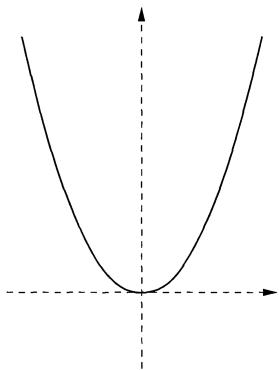
\includegraphics[width=0.42\textwidth]{figs/ch7-parabola.jpg}\qquad
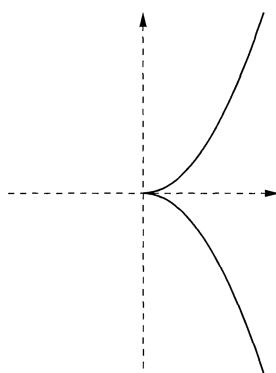
\includegraphics[width=0.42\textwidth]{figs/ch7-cusp.jpg}
\end{center}

第一个是 $\mathcal{V}((y-x^2))$; 第二个是 $\mathcal{V}((y^2-x^3))$. 理想 $(y^2-x^3)$ 的什么性质造成了第二幅图中 $(0,0)$ 处的``尖点''? 读者在任何一门初等代数几何课程中都会找到答案.
\end{example}

$\mathcal{I}$ 不满射这一事实引出了一些有趣的思考. 不是任何集合之理想的理想的标准例子是 $K[x]$ 中的 $(x^2)$: 因为凡是 $x^2$ 消失的地方, $x$ 也消失; 所以若对某个集合 $S$ 有 $x^2\in\mathcal{I}(S)$, 则也有 $x\in\mathcal{I}(S)$. 这引出下面的定义.

\begin{definition}\label{def:radical}
设 $I$ 是交换环 $R$ 中的一个理想. $I$ 的\emph{根}\index{gen@根(radical)}是理想
\[
\sqrt{I}:=\{r\in R\mid \exists k\geq 0,\ r^k\in I\}.
\]
一个理想 $I$ 是\emph{根理想}\index{gen lixiang@根理想(radical ideal)}, 如果 $I=\sqrt{I}$.
\end{definition}

读者应当验证 $\sqrt{I}$ 确实是一个理想; 它可以刻画为所有包含 $I$ 的素理想的交 (习题~\ref{ex:radical-props}).

\begin{example}\label{ex:nilradical-example}
交换环 $R$ 中的一个元素是幂零的, 当且仅当它属于理想 $(0)$ 的根 (对照习题~V.\ref{ex:nilpotent-unit}). 读者已经在习题中遇到过这个理想, 称为 $R$ 的\emph{幂零根}, 从习题~III.\ref{ex:nilradical} 开始.

素理想 $\mathfrak{p}$ 显然是根理想: 因为 $f^k\in\mathfrak{p}\implies f\in\mathfrak{p}$, 从而 $\sqrt{\mathfrak{p}}\subseteq\mathfrak{p}$ (另一个包含关系对一切理想都平凡地成立).
\end{example}

\begin{lemma}\label{lem:ideal-of-set-radical}
设 $K$ 是一个域, 并设 $S$ 是 $\mathbb{A}_K^n$ 的一个子集. 则理想 $\mathcal{I}(S)$ 是 $K[x_1,\ldots ,x_n]$ 的一个根理想.
\end{lemma}

\begin{proof}
包含关系 $\mathcal{I}(S)\subseteq\sqrt{\mathcal{I}(S)}$ 对每个理想都成立, 所以平凡地满足. 为验证包含关系 $\sqrt{\mathcal{I}(S)}\subseteq\mathcal{I}(S)$, 设 $f\in\sqrt{\mathcal{I}(S)}$. 则存在整数 $k\geq 0$ 使得 $f^k\in\mathcal{I}(S)$; 也就是说,
\[
(\forall p\in S),\quad f(p)^k=0.
\]
于是
\[
(\forall p\in S),\quad f(p)=0,
\]
这就证明了 $f\in\mathcal{I}(S)$, 正是所需要的. \qed
\end{proof}

鉴于这些考虑, 对任意域我们可以把 $\mathbb{A}_K^n$ 的子集与 $K[x_1,\ldots ,x_n]$ 的理想之间的对应精化如下:
\[
\begin{tikzcd}[column sep=3em]
\{\mathbb{A}_K^n\text{ 的代数子集}\} \ar[r,shift left=.7ex,"\mathcal I"] & \{K[x_1,\ldots ,x_n]\text{ 中的根理想}\}; \ar[l,shift left=.7ex,"\mathcal V"]
\end{tikzcd}
\]
正如我们论证过的, 如果想要有一部好的词典, 这样做是必要的. 在本节余下部分, $\mathcal{I}$ 与 $\mathcal{V}$ 将被看作在这两个集合之间作用.

虽然我们已经把这个对应大大收紧了, 情况仍不完美. 在任意域上, 函数 $\mathcal{V}$ 现在按仿射代数子集的定义是满射 (对照习题~\ref{ex:alg-set-radical-ideal}); 但它不一定是单射. 一个立刻的反例由 $K=\R$ 上的理想 $(x^2+1)$ 给出: 它是极大的, 从而是素的, 从而是根理想, 而
\[
\mathcal{V}(x^2+1)=\emptyset=\mathcal{V}(1).
\]

零点定理正是在这里来帮助我们, 而我们也正是在这里看到零点定理与一个理想的``零点'' (= 该理想的 $\mathcal{V}$) 有什么关系.

\begin{proposition}[弱零点定理]\label{prop:weak-nullstellensatz}
设 $K$ 是代数闭域, 并设 $I\subseteq K[x_1,\ldots ,x_n]$ 是一个理想. 则 $\mathcal{V}(I)=\emptyset$ 当且仅当 $I=(1)$.
\end{proposition}

\begin{proof}
若 $I=(1)$, 则按定义 $\mathcal{V}(I)=\emptyset$.

反过来, 假设 $I\neq (1)$. 由命题~V.\ref{prop:maximal-ideal-exists}, $I$ 包含在一个极大理想 $\mathfrak{m}$ 中. 由于 $K$ 是代数闭的, 由推论~\ref{cor:maximal-ideals-points} 我们有
\[
\mathfrak{m}=(x_1-c_1,\ldots ,x_n-c_n)
\]
其中 $c_1,\ldots ,c_n\in K$; 所以对每个 $f(x_1,\ldots ,x_n)\in I$ 存在 $g_1,\ldots ,g_n\in K[x_1,\ldots ,x_n]$ 使得
\[
f(x_1,\ldots ,x_n)=\sum_{i=1}^{n}g_i(x_1,\ldots ,x_n)(x_i-c_i).
\]\erratumfootnote{根据官方勘误, 公式中多项式因子记号统一修正为 $g_i$.}
特别地,
\[
f(c_1,\ldots ,c_n)=\sum_{i=1}^{n}g_i(c_1,\ldots ,c_n)(c_i-c_i)=0:
\]
也就是说, $(c_1,\ldots ,c_n)\in\mathcal{V}(I)$. 这就证明了当 $I\neq (1)$ 时 $\mathcal{V}(I)\neq\emptyset$, 证毕. \qed
\end{proof}

这令人鼓舞, 但它似乎并没有真正证明 $\mathcal{V}$ 是单射. 然而事实是, 它确实证明了: 我们可以从``弱''零点定理推出下面这个更强的结果, 而后者确实蕴涵单射性:

\begin{proposition}[强零点定理]\label{prop:strong-nullstellensatz}
设 $K$ 是代数闭域, 并设 $I\subseteq K[x_1,\ldots ,x_n]$ 是一个理想. 则
\[
\mathcal{I}(\mathcal{V}(I))=\sqrt{I}.
\]
\end{proposition}

这意味着复合 $\mathcal{I}\circ\mathcal{V}$ 在根理想集合上是恒等映射; 也就是说, $\mathcal{V}$ 有一个左逆, 从而它是单射 (对照命题~I.\ref{prop:left-right-inverse}!).

\begin{proof}
注意 $\mathcal{I}(\mathcal{V}(I))$ 是一个根理想 (由引理~\ref{lem:ideal-of-set-radical}). 由定义立刻有 $I\subseteq\mathcal{I}(\mathcal{V}(I))$; 因此
\[
\sqrt{I}\subseteq\sqrt{\mathcal{I}(\mathcal{V}(I))}=\mathcal{I}(\mathcal{V}(I)).
\]
我们必须验证反过来的包含关系: 假设 $f\in\mathcal{I}(\mathcal{V}(I))$; 也就是说, 假设
\[
f(p)=0
\]
对所有满足 $\forall g\in I,\ g(p)=0$ 的 $p\in\mathbb{A}_K^n$ 成立; 我们要证明存在 $m$ 使得 $f^m\in I$.

这个论证在事后看来并不困难, 但它极其巧妙\footnote{这称为 Rabinowitsch 技巧, 可追溯到 1929 年. 它发表于《Mathematische Annalen》上一篇仅一页、十八行的文章中.}. 令 $y$ 是一个额外的变量, 考虑 $K[x_1,\ldots ,x_n,y]$ 中由 $I$ 与 $1-fy$ 生成的理想 $J$. 更明确地, 假设
\[
I=(g_1,\ldots ,g_r)
\]
(由于 $K[x_1,\ldots ,x_n]$ 是 Noether 的, 有限多个生成元就够了); 我们可以把 $g_i(x_1,\ldots ,x_n)$ 与 $f(x_1,\ldots ,x_n)\in K[x_1,\ldots ,x_n]$ 分别看成多项式 $G_i(x_1,\ldots ,x_n,y)$ 与 $F(x_1,\ldots ,x_n,y)\in K[x_1,\ldots ,x_n,y]$, 并令
\[
J=(G_1,\ldots ,G_r,1-Fy).
\]
由于 $K[x_1,\ldots ,x_n,y]$ 有 $n+1$ 个变量, 理想 $J$ 定义了 $\mathbb{A}_K^{n+1}$ 中的一个子集 $\mathcal{V}(J)$. 我们断言 $\mathcal{V}(J)=\emptyset$.

确实, 反设 $\mathcal{V}(J)\neq\emptyset$, 并设 $p=(a_1,\ldots ,a_n,b)\in\mathbb{A}_K^{n+1}$ 是 $\mathcal{V}(J)$ 的一个点. 那么对 $i=1,\ldots ,r$ 有
\[
G_i(a_1,\ldots ,a_n,b)=0;
\]
但这意味着
\[
g_i(a_1,\ldots ,a_n)=0
\]
对 $i=1,\ldots ,r$ 成立; 也就是说, $(a_1,\ldots ,a_n)\in\mathcal{V}(I)$. 由于 $f$ 在 $\mathcal{V}(I)$ 的所有点上都消失, 这意味着
\[
f(a_1,\ldots ,a_n)=0,
\]
于是
\[
(1-Fy)(a_1,\ldots ,a_n,b)=1-f(a_1,\ldots ,a_n)b=1-0=1.
\]
但这与 $p\in\mathcal{V}(J)$ 的假设矛盾. 因此 $\mathcal{V}(J)=\emptyset$.

现在使用弱零点定理: 由于 $K$ 是代数闭的, 我们可以断定 $J=(1)$. 因此存在多项式 $H_i(x_1,\ldots ,x_n,y)$ ($i=1,\ldots ,r$) 与 $L(x_1,\ldots ,x_n,y)$, 使得
\[
\sum_{i=1}^{r}H_i(x_1,\ldots ,x_n,y)G_i(x_1,\ldots ,x_n,y)+L(x_1,\ldots ,x_n,y)\bigl(1-F(x_1,\ldots ,x_n,y)y\bigr)=1.
\]
我们的巧妙还没有结束: 下一步是在 $K$ 上的有理函数域中 (而不是在多项式环中) 看待这个等式, 我们这样做是可以的, 因为后者是前者的子环. 于是我们可以代入 $y=1/F$ 而仍然得到一个等式, 好处是消掉了左边最后一项:
\[
\sum_{i=1}^{r}H_i\left(x_1,\ldots ,x_n,\frac{1}{F}\right)G_i\left(x_1,\ldots ,x_n,\frac{1}{F}\right)=1.
\]
进而,
\[
G_i\left(x_1,\ldots ,x_n,\frac{1}{F}\right)=g_i(x_1,\ldots ,x_n)
\]
($G_i$ 只是 $g_i$ 在更大的多项式环中的名字, 并且只依赖前 $n$ 个变量), 而
\[
H_i\left(x_1,\ldots ,x_n,\frac{1}{F}\right)=\frac{h_i(x_1,\ldots ,x_n)}{f(x_1,\ldots ,x_n)^m},
\]
其中 $h_i\in K[x_1,\ldots ,x_n]$, 而 $m$ 是一个大到对所有 $i=1,\ldots ,r$ 都适用的整数. 用通分表示, 我们可以把这个恒等式重写为
\[
\frac{h_1g_1+\cdots +h_rg_r}{f^m}=1,
\]
或
\[
f^m=h_1g_1+\cdots +h_rg_r.
\]
我们是在有理函数域中证明这个恒等式的; 由于它只涉及多项式, 它在 $K[x_1,\ldots ,x_n]$ 中成立. 右边是 $I$ 的一个元素, 所以这证明了 $f\in\sqrt{I}$, 证毕. \qed
\end{proof}

证明中添加变量 $y$ 的做法, 如果从几何角度来看, 就显得更合理 (也不那么像一个花招). $\mathbb{A}_K^2$ 中的簇 $\mathcal{V}(1-xy)$ 是一条普通的双曲线:

\begin{center}
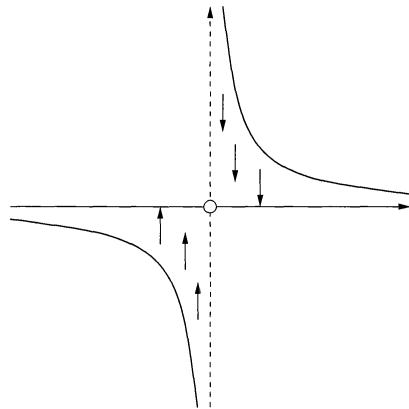
\includegraphics[width=0.5\textwidth]{figs/ch7-hyperbola.jpg}
\end{center}

投影 $(x,y)\mapsto x$ 可用来把 $\mathcal{V}(1-xy)$ 与``$x$ 轴'' (看作 $\mathbb{A}_K^1$) 中原点 (即 $\mathcal{V}(x)$) 的补集等同起来. 类似地, $\mathcal{V}(1-fy)$ 是把 Zariski 开集 $\mathbb{A}_K^n\setminus\mathcal{V}(f)$ 实现为维数高一维的空间 $\mathbb{A}_K^{n+1}$ 中一个 Zariski 闭子集的一种方式.

命题~\ref{prop:strong-nullstellensatz} 的证明正依赖于这个事实, 而这个事实也是代数几何基本框架中的一个重要构件, 因为它可以用来证明 Zariski 拓扑有一组由 (在适当意义上同构于) 仿射代数集的集合构成的基.

我们将正式记录下关于函数 $\mathcal{V}$ 与 $\mathcal{I}$ 所能确立的结论:

\begin{corollary}\label{cor:agc-dictionary}
设 $K$ 是代数闭域. 则对任意 $n\geq 0$, 函数
\[
\begin{tikzcd}[column sep=3em]
\{\mathbb{A}_K^n\text{ 的代数子集}\} \ar[r,shift left=.7ex,"\mathcal I"] & \{K[x_1,\ldots ,x_n]\text{ 中的根理想}\} \ar[l,shift left=.7ex,"\mathcal V"]
\end{tikzcd}
\]
互为逆映射.
\end{corollary}

\begin{proof}
命题~\ref{prop:strong-nullstellensatz} 表明 $\mathcal{I}\circ\mathcal{V}$ 在根理想上是恒等映射, 所以 $\mathcal{V}$ 是单射, 而 $\mathcal{V}$ 按仿射代数集的定义是满射. 由此 $\mathcal{V}$ 是双射而 $\mathcal{I}$ 是它的逆. \qed
\end{proof}

\noindent\emph{总结.} 若 $K$ 是代数闭的, 则在空间 $K^n$ 中研究由多项式方程定义的集合, 与在多项式环 $K[x_1,\ldots ,x_n]$ 中研究根理想是``同一件事''.

这个对应实际上在 $K$-代数的层面上实现得更为有效. 我们说一个环是\emph{既约的}\index{jiyue@既约的(reduced)}, 如果它没有非零的幂零元; 于是 $R/I$ 是既约的当且仅当 $I$ 是根理想 (习题~\ref{ex:radical-props}).

\begin{definition}\label{def:coordinate-ring}
设 $S\subseteq\mathbb{A}_K^n$ 是一个代数集. $S$ 的\emph{坐标环}\index{zuobiaohuan@坐标环(coordinate ring)}是商\footnote{记号 $K[S]$ 相当标准, 尽管它可能与通常的多项式环记号混淆; 希望上下文足以消除歧义. 把域的名字写在记号中是合理的, 因为原则上可以改变基域, 同时保留理想 $\mathcal I(S)$ 所编码的``相同''方程.}
\[
K[S]:=\frac{K[x_1,\ldots ,x_n]}{\mathcal{I}(S)}.
\]
\end{definition}

\index{daishujidezuobiaohuan@代数集的坐标环(coordinate ring of an algebraic set)}于是, 一个代数集的坐标环是一个既约的、有限型的交换 $K$-代数. 读者将在习题~\ref{ex:polynomial-functions} 中建立这个环的一个``具体''解释, 即作为 $S$ 上``多项式函数''的环. 理解零点定理 (以其作为推论~\ref{cor:agc-dictionary} 的表现形式) 的一种方式是这样: 若 $K$ 是代数闭的, 则每个有限型既约交换 $K$-代数 $R$ 都可以实现为某个仿射代数集 $S$ 的坐标环; $S$ 的点以一种自然的方式对应于 $R$ 的极大理想 (习题~\ref{ex:points-maximal-ideals}).

事实上\footnote{这当然是对实际情况的极度简化.}, 在基础代数几何中, 人们正是通过这一对应来定义一个域 $K$ 上的仿射代数集的范畴: 代数集的态射被定义为与相应的 (既约、有限型) $K$-代数的同态相匹配. (读者将在例~VIII.\ref{ex:k-aff} 中遇到一个更精确的定义.)

这部词典使我们能够把一个代数集的每个``几何''特征 (例如维数、光滑性等等) 翻译成相应的坐标环的对应``代数''特征. 一旦这些关键的代数特征被辨认出来, 人们就可以抛开``在代数闭域上的既约有限型代数上工作''这一限制, 尝试在任意 (比如说交换的、Noether 的) 环上``做几何''. 例如, 结果发现 PID 对应于仿射几何世界中的 (某些) 光滑曲线; 于是人们可以尝试把 $\Z$ 想象成一条``光滑曲线'' (尽管 $\Z$ 不是任何域 $K$ 上的既约有限型 $K$-代数!) 并尝试使用受曲线几何启发的定理来理解 $\Z$ 的特征——也就是说, 用几何来做数论.

\index{pu@谱(spectrum)!huande@环的(of a ring)}这些简单的考虑可以被推广的另一个方向, 是通过把仿射代数集``粘合''成类似流形的对象: 这些集合在``整体''上可能不是仿射代数集, 但可以被仿射代数集覆盖. 做这件事的一个具体办法是在射影空间而不是仿射空间中工作; 整体化的过程于是可以在代数层面以一种直接的方式进行, 在那里它被翻译为对``分次''环与模的研究——更多遗憾地在我们这本书中找不到位置的概念 (只在 §VIII.\ref{subsec:graded-algebra} 中匆匆一瞥). 在二十世纪下半叶, 一个由 Alexander Grothendieck 等人倡导的更抽象的观点被证明极为有效; 它导致了对概形\index{guaixing@概形(scheme)}——代数几何当今通用的语言——的深入研究. 我们早在 §III.\ref{subsec:prime-maximal-def} 引入环的谱 $\Spec R$ 时, 就已经遇到过最简单的一类概形.

\subsection*{习题}
\phantomsection
\addcontentsline{toc}{subsection}{习题}

\begin{prob}\label{ex:alg-closed-equiv-proof}
$\triangleright$ 证明引理~\ref{lem:alg-closed-equiv}. [§\ref{subsec:algebraic-closure}]
\end{prob}

\begin{prob}\label{ex:alg-closure-minimal}
$\triangleright$ 设 $k\subseteq\overline{k}$ 是一个代数闭包, 并设 $L$ 是一个中间域. 假设每个多项式 $f(x)\in k[x]\subseteq L[x]$ 都在 $L[x]$ 中分解为一次因子的乘积. 证明 $L=\overline{k}$. [§\ref{subsec:algebraic-closure}]
\end{prob}

\begin{prob}\label{ex:countable-closure}
证明若 $k$ 是可数域, 则 $\overline{k}$ 也是可数的.
\end{prob}

\begin{prob}\label{ex:partial-fractions-nonzero}
$\triangleright$ 设 $k$ 是一个域, 设 $c_1,\ldots ,c_m\in k$ 是互异元素, 并设 $\lambda_1,\ldots ,\lambda_m$ 是 $k$ 的非零元素. 证明
\[
\frac{\lambda_1}{x-c_1}+\cdots +\frac{\lambda_m}{x-c_m}\neq 0.
\]
(这个事实用在定理~\ref{thm:nullstellensatz} 的证明中.) [§\ref{subsec:nullstellensatz}]
\end{prob}

\begin{prob}\label{ex:V-of-ideal-generated}
$\triangleright$ 设 $K$ 是一个域, 设 $A$ 是 $K[x_1,\ldots ,x_n]$ 的一个子集, 并设 $I$ 是 $A$ 生成的理想. 证明在 $\mathbb{A}_K^n$ 中 $\mathcal{V}(A)=\mathcal{V}(I)$. [§\ref{subsec:affine-geometry}]
\end{prob}

\begin{prob}\label{ex:non-algebraic-subsets}
$\triangleright$ 设 $K$ 是你最喜欢的无限域. 找出不能实现为任何理想 $I\subseteq K[x_1,\ldots ,x_n]$ 的 $\mathcal{V}(I)$\erratumfootnote{根据官方勘误, 原书此处规范代数集算子符号为花体字形 $\mathscr{V}(I)$.} 的子集 $S\subseteq\mathbb{A}_K^n$ 的例子. 证明若 $K$ 是有限域, 则每个子集 $S\subseteq\mathbb{A}_K^n$ 都等于某个理想 $I\subseteq K[x_1,\ldots ,x_n]$ 的 $\mathcal{V}(I)$. [§\ref{subsec:affine-geometry}]
\end{prob}

\begin{prob}\label{ex:zariski-topology}
$\triangleright$ 设 $K$ 是一个域而 $n$ 是一个非负整数. 证明 $\mathbb{A}_K^n$ 的代数子集族是 $\mathbb{A}_K^n$ 上某个拓扑的闭集族. [§\ref{subsec:affine-geometry}]
\end{prob}

\begin{prob}\label{ex:radical-props}
$\triangleright$ 采用定义~\ref{def:radical} 中的记号:
\begin{itemize}
\item 证明集合 $\sqrt{I}$ 是 $R$ 的一个理想.
\item 通过 $R/I$ 的理想与 $R$ 中包含 $I$ 的理想之间的对应, 证明 $\sqrt{I}$ 对应于 $R/I$ 的幂零根.
\item 证明 $\sqrt{I}$ 事实上是所有包含 $I$ 的 $R$ 的素理想的交. (对照习题~V.\ref{ex:nilradical-prime-intersection}.)
\item 证明 $I$ 是根理想当且仅当 $R/I$ 是既约的. (对照习题~III.\ref{ex:reduced}.)
\end{itemize}
[§\ref{subsec:affine-geometry}]
\end{prob}

\begin{prob}\label{ex:alg-set-radical-ideal}
$\triangleright$ 证明每个仿射代数集都等于某个根理想 $I$ 的 $\mathcal{V}(I)$. [§\ref{subsec:affine-geometry}]
\end{prob}

\begin{prob}\label{ex:noetherian-power-radical}
\index{Noether@Noether!huan@环(ring)}证明 Noether 环中的每个理想都含有它的根的某个幂.
\end{prob}

\begin{prob}\label{ex:reduced-not-coordinate}
假设一个域不是代数闭的. 找出一个既约的有限型 $K$-代数, 它不是任何仿射代数集的坐标环.
\end{prob}

\begin{prob}\label{ex:polynomial-functions}
$\triangleright$ 设 $K$ 是无限域. 仿射代数集 $S\subseteq\mathbb{A}_K^n$ 上的一个\emph{多项式函数}, 是一个多项式 $f(x_1,\ldots ,x_n)\in K[x_1,\ldots ,x_n]$ 的 (求值函数的) 在 $S$ 上的限制. 代数集 $S$ 上的多项式函数显然构成一个环, 而且事实上是一个 $K$-代数. 证明这个 $K$-代数同构于 $S$ 的坐标环. [§\ref{subsec:affine-geometry}, §VIII.\ref{subsec:equiv-categories}, §VIII.\ref{subsec:tensor-flatness}]
\end{prob}

\begin{prob}\label{ex:reduced-fg-is-coordinate}
设 $K$ 是代数闭域. 证明每个有限型既约交换 $K$-代数都是某个仿射空间 $\mathbb{A}_K^n$ 中一个代数集 $S$ 的坐标环.
\end{prob}

\begin{prob}\label{ex:points-maximal-ideals}
$\triangleright$ 证明在代数闭域 $K$ 上, 一个代数集 $S$ 的点对应于坐标环 $K[S]$ 的极大理想, 并且若 $p$ 对应于极大理想 $\mathfrak{m}_p$, 则函数 $f\in K[S]$ 在 $p$ 处的值等于 $f$ 在 $K[S]/\mathfrak{m}_p\cong K$ 中的陪集. [§\ref{subsec:affine-geometry}, VIII.\ref{ex:k-aff-points}]
\end{prob}

\begin{prob}\label{ex:irreducible-prime}
$\neg$ 设 $K$ 是代数闭域. $\mathbb{A}_K^n$ 的一个代数子集 $S$ 是\emph{不可约的}\index{bukeyue@不可约的(irreducible)}, 如果它不能写成两个真包含于它的代数子集的并. 证明 $S$ 不可约当且仅当它的理想 $\mathcal{I}(S)$ 是素理想, 当且仅当它的坐标环 $K[S]$ 是整环.

不可约代数集``浑然一体'', 就像 $\mathbb{A}_K^n$ 自己那样, 而不像 (例如) 以 $x,y$ 为坐标的仿射平面 $\mathbb{A}_K^2$ 中的 $\mathcal{V}(xy)$. 不可约的仿射代数集称为\emph{(仿射代数) 簇}. [\ref{ex:cusp-coordinate-rings}]
\end{prob}

\begin{prob}\label{ex:rational-functions-localization}
$\triangleright$ 设 $K$ 是代数闭域. 有理函数域 $K(x_1,\ldots ,x_n)$ 是 $K[\mathbb{A}_K^n]=K[x_1,\ldots ,x_n]$ 的分式域; 每个有理函数 $\alpha=F/G$ (其中 $G\neq 0$ 且 $F,G$ 互素) 都可以看作在开集 $\mathbb{A}_K^n\setminus\mathcal{V}(G)$ 上定义了一个函数; 我们说 $\alpha$ 对 $\mathcal{V}(G)$ 的补集中的所有点都``有定义''.

设 $G\in K[x_1,\ldots ,x_n]$ 不可约. 在 $\mathcal{V}(G)$ 的补集中有定义的有理函数的集合是 $K(x_1,\ldots ,x_n)$ 的一个子环. 证明这个子环可以等同于 $K[\mathbb{A}_K^n]$ 在乘性集合 $\{1,G,G^2,G^3,\ldots \}$ 处的局部化 (习题~V.\ref{ex:localization-ring}). (使用零点定理.)
[\ref{ex:germs-localization}, \ref{ex:rational-function-fields-curves}, \S\ref{subsec:ft-galois-II}]
\end{prob}

\begin{prob}\label{ex:germs-localization}
$\neg$ 设 $K$ 是代数闭域, 并设 $\mathfrak{m}$ 是 $K[x_1,\ldots ,x_n]$ 的一个极大理想, 对应于 $\mathbb{A}_K^n$ 的一个点 $p$. 一个函数在 $p$ 处的\emph{芽}\index{ya@芽(germ)}, 由一个包含 $p$ 的开集以及定义在该开集上的一个函数确定; 在我们的语境中 (处理有理函数, 并且开集可以取为一个在 $p$ 处不消失的函数的补集), 这与一个在 $p$ 处有定义的有理函数 (在习题~\ref{ex:rational-functions-localization} 的意义下) 是同一份信息.

说明如何把芽环等同于局部化 $K[\mathbb{A}_K^n]_{\mathfrak{m}}$ (在习题~V.\ref{ex:local-ring} 中定义).

如同习题~\ref{ex:rational-functions-localization} 那样, 同样的讨论可以对任意代数集进行. 这就是``局部化''这个名字的由来: 把一个簇 $V$ 的坐标环在对应于点 $p$ 的极大理想处局部化, 相当于只考虑在 $p$ 的某个邻域中有定义的函数, 从而也就是在 $p$ ``附近''``局部地''研究 $V$. [V.\ref{ex:localization-ring}]
\end{prob}

\begin{prob}\label{ex:cusp-coordinate-rings}
$\neg$ 设 $K$ 是代数闭域. 考虑 $\mathbb{A}_K^2$ 中的两条``曲线'' $C_1:y=x^2$ 与 $C_2:y^2=x^3$ (这些代数集的实点图像见例~\ref{ex:cusp}).
\begin{itemize}
\item 证明 $K[C_1]\cong K[t]=K[\mathbb{A}_K^1]$, 而 $K[C_2]$ 可以等同于 $K[t]$ 的由 $t$-系数为零的多项式 $a_0+a_2t^2+\cdots +a_dt^d$ 组成的子环 $K[t^2,t^3]$. (注意 $K[x,y]$ 中每个多项式都可以唯一地写成 $f(x)+g(x)y+h(x,y)(y^2-x^3)$ 的形式, 其中 $f(x)$, $g(x)$, $h(x,y)$ 由该多项式唯一确定.)
\item 证明 $C_1$, $C_2$ 都是不可约的 (对照习题~\ref{ex:irreducible-prime}).
\item 证明 $K[C_1]$ 是 UFD, 而 $K[C_2]$ 不是.
\item 证明 $K[C_1]$ 与 $K[C_2]$ 的 Krull 维数都是 $1$. (这就是为什么这些集合会被称为``曲线''. 你可以使用如下事实: $K[x,y]$ 中的素理想极大链长度为 $2$.)
\item 原点 $(0,0)$ 同时在 $C_1$ 与 $C_2$ 中, 并且分别对应于 $K[C_1]$ 与 $K[C_2]$ 中由 $x$ 与 $y$ 的陪集生成的极大理想 $\mathfrak{m}_1$ 与 $\mathfrak{m}_2$.
\item 证明局部化 $K[C_1]_{\mathfrak{m}_1}$ 是一个 DVR (习题~V.\ref{ex:pid-localization-dvr}). 证明局部化 $K[C_2]_{\mathfrak{m}_2}$ 不是 DVR. (注意关系 $y^2=x^3$ 在这个环中仍然成立; 证明 $K[C_2]_{\mathfrak{m}_2}$ 不是 UFD.)
\end{itemize}
DVR 容许一个局部参数, 即它的极大理想的一个生成元 (对照习题~V.\ref{ex:dvr-pid-localparam}), 这个事实是如下几何事实的一个很好的代数翻译: 像 $C_1$ 这样的一条曲线在 $(0,0)$ 处只有一条光滑的分支. $K[C_2]_{\mathfrak{m}_2}$ 的极大理想不能只由一个元素生成, 读者可以自行验证. [\ref{ex:rational-function-fields-curves}]
\end{prob}

\begin{prob}\label{ex:rational-function-fields-curves}
证明习题~\ref{ex:cusp-coordinate-rings} 中曲线 $C_1$ 与 $C_2$ 的有理函数域 (习题~\ref{ex:rational-functions-localization}) 同构, 并且它们在 $k$ 上的超越次数都是 $1$ (对照习题~\ref{ex:transcendence-basis}).

这是我们应当把 $C_1$ 与 $C_2$ 看作``曲线''的另一个理由. 事实上, 可以证明一个簇的坐标环的 Krull 维数等于它的有理函数域的超越次数. 这是交换代数的一块基石——Noether 归一化定理——的一个推论.
\end{prob}

\begin{prob}\label{ex:projective-cover}
$\neg$ 回顾习题~VI.\ref{ex:grassmannian-cells}: $\mathbb{P}_K^n$ 表示参数化向量空间 $K^{n+1}$ 中直线的``射影空间''. 每条这样的直线由某个非零向量 $(c_0,\ldots ,c_n)\in K^{n+1}$ 的所有倍数组成, 于是 $\mathbb{P}_K^n$ 可以等同于 $K^{n+1}\setminus\{(0,\ldots ,0)\}$ 关于等价关系 $\sim$ 的商 (在 §I.\ref{subsec:equivalence-relations} 的集合论意义下), 其中 $\sim$ 定义为\index[sym1]{46@$\mathbb{P}_K^n$}
\[
(c_0,\ldots ,c_n)\sim (c_0',\ldots ,c_n')\iff (\exists \lambda\in K^{*}),\ (c_0',\ldots ,c_n')=(\lambda c_0,\ldots ,\lambda c_n).
\]
由向量 $(c_0,\ldots ,c_n)$ 确定的 $\mathbb{P}_K^n$ 中的``点''记作 $(c_0:\cdots :c_n)$; 这些是该点的``射影坐标''\footnote{这是方便的记号滥用. 请记住, $c_i$ 并不由这个点确定, 因而严格来说并不是``坐标''; 不过它们的比值由这个点确定.}. 注意不存在``点'' $(0:\cdots :0)$.\index[sym1]{09@$(c_0:\cdots:c_n)$}

证明由
\[
(c_1,\ldots ,c_n)\mapsto (1:c_1:\cdots :c_n)
\]
定义的函数 $\mathbb{A}_K^n\to\mathbb{P}_K^n$ 是到其像上的双射\erratumfootnote{根据官方勘误, 原书英文此处由 ``is a bijection'' 修正为 ``is a bijection onto its image''.}. 这个函数被用来把 $\mathbb{A}_K^n$ 实现为 $\mathbb{P}_K^n$ 的一个子集. 通过使用类似的函数, 证明 $\mathbb{P}_K^n$ 可以被 $n+1$ 份 $\mathbb{A}_K^n$ 的拷贝覆盖, 并把这个事实与习题~VI.\ref{ex:grassmannian-cells} 中得到的胞腔分解联系起来. (建议: 仔细地做一遍 $n=2$ 的情形.) [\ref{ex:projective-algebraic-set}, VIII.\ref{ex:plucker-equations}]
\end{prob}

\begin{prob}\label{ex:projective-algebraic-set}
$\neg$ 设 $F(x_0,\ldots ,x_n)\in K[x_0,\ldots ,x_n]$ 是一个齐次多项式. 采用习题~\ref{ex:projective-cover} 中的记号, 证明对点 $(c_0:\cdots :c_n)\in\mathbb{P}_K^n$ 而言条件``$F(c_0,\ldots ,c_n)=0$''是良定义的: 它不依赖于为该点所选取的代表元 $(c_0,\ldots ,c_n)$. 于是我们可以定义 $\mathbb{P}_K^n$ 的如下子集:
\[
\mathcal{V}(F):=\{(c_0:\cdots :c_n)\in\mathbb{P}_K^n\mid F(c_0,\ldots ,c_n)=0\}.
\]
证明这个``射影代数集''可以被 $n+1$ 个仿射代数集覆盖.

``射影代数几何''中的基本定义可以沿着与本节为仿射代数几何所走的道路本质相同的路线来发展, 只不过使用``齐次理想'' (即由齐次多项式生成的理想; 见 §VIII.\ref{subsec:graded-algebra}) 而不是普通的理想. 这道习题展示了在一个模板例子中把射影代数集与仿射代数集联系起来的一种方式. [VIII.\ref{ex:plucker-equations}, VIII.\ref{ex:projective-variety}]
\end{prob}

\section{几何不可能性}
\label{sec:geometric-impossibilities}

域论中一些非常简单的考察, 就能轻松了结一大类长期以来似乎无从下手的几何问题——这些问题曾困扰希腊人, 直到相对晚近才被解决.

\index{chiguizuotu@尺规作图(straightedge-and-compass constructions)}这些问题关乎用``直尺与圆规'' (亦即服从某些非常严格的规则) 去作某些几何图形. 这些作图的实际用途看来绝对为零, 但是, 对于那些曾经难住了极其聪明的头脑、而我们如今却能彻底理解的事情, 由此获得的智识上的满足, 值得为此小小的绕道一行.

\subsection{直尺与圆规作图}
\label{subsec:straightedge-compass}

我们从普通实平面上的两个点 $O$, $P$ 出发. 允许你在平面中标记 (``作'') 更多的点与其他几何图形, 但只能依照下列规则:

\begin{itemize}
\item 如果你已经作出了两个点 $A$, $B$, 那么你可以作过这两点的直线 (用你的直尺).
\item 如果你已经作出了两个点 $A$, $B$, 那么你可以作以 $A$ 为圆心且经过 $B$ 的圆 (用你的圆规).
\item 你可以标记任意多个你已经作出的两条不同直线, 一条直线和一个圆, 或两个不同圆的交点.
\end{itemize}

施行这些动作会产生复杂 (而优美) 的直线与圆的集合; 如果某个图形作为整个画面的一部分出现, 我们就说我们``作出了''它.

例如, 下面是用 $O$, $P$ 作为其中两个顶点来作等边三角形的一个方案:

\begin{enumerate}
\item[(1)] 作以 $O$ 为圆心, 经过 $P$ 的圆;
\item[(2)] 作以 $P$ 为圆心, 经过 $O$ 的圆;
\item[(3)] 令 $Q$ 为这两个圆的两个交点中的任意一个;
\item[(4)] 作过 $O$, $P$; 过 $O$, $Q$; 以及过 $P$, $Q$ 的直线.
\end{enumerate}

\begin{center}
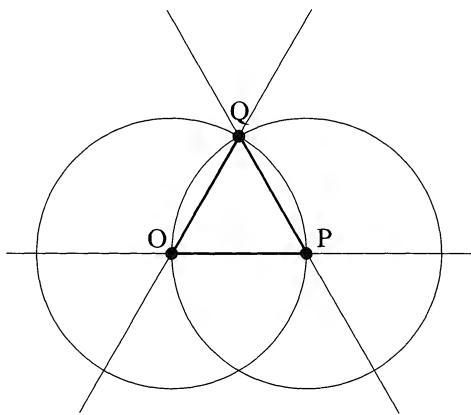
\includegraphics[width=0.5\textwidth]{figs/ch7s3-01.jpg}
\end{center}

当然, $O$, $P$, $Q$ 是一个等边三角形的顶点.

尝试给出作出某个给定图形或几何构型的具体的基本步骤序列, 是一个愉快的练习. 富有进取心的读者可以在不查资料, 并且在我们学到足够多以至于挫败纯粹几何直觉之前, 试着用直尺与圆规作出正五边形的顶点.

一般的问题是判断一个图形能不能用这种方式作出. 下述三类问题在古代就声名远扬:

\begin{itemize}
\item 三等分角;
\item 化圆为方;
\item 倍立方.
\end{itemize}

例如, 假设已经作出了两条形成角 $\theta$ 的直线, 问能否作出两条形成角 $\theta/3$ 的直线. 对某些可构造的 $\theta$ 这显然是可能的: 我们刚刚作出了一个 $\pi/3$ 的角, 所以显然我们能够三等分角 $\pi$; 但是这对所有可构造的角都能做到吗?

\index{kegouzao@可构造(constructible)}答案是否定的. 类似地, 不可能作出与一个 (可构造的) 圆面积相同的正方形, 也不可能作出边长等于一个给定 (可构造) 边长立方体之体积两倍的立方体的棱.

\index{zhengduobianxing@正多边形(regular polygon)!dekegouzaoxing@的可构造性(constructibility of a)}域论将使我们能够确立这一切\footnote{不过, 为证明化圆为方不可能, 我们将用到 $\pi$ 的超越性; 本书不证明这一事实.}.\index{zhichi yu yuan gui@直尺与圆规(straightedge and compass)} 稍后我们会回到这些作图, 并研究给定边长的正多边形的可构造性问题: 用直尺与圆规作出等边三角形 (我们刚刚做过), 正方形, 正六边形都极易; 作出正五边形也不太难; 但是哪些多边形可构造, 哪些不可构造, 却与域论中更深刻的问题优美地联系在一起.

上述三类问题有一段显赫的历史; 如果阿里斯托芬《鸟》中的这一残篇可作凭据, 它们至少可以追溯到公元前414年:

\begin{quote}
METON: 用直尺一量, 这圆就成了一个带内院的方.\footnote{感谢 Matilde Marcolli 提供翻译. 对于比我更懂希腊语的读者, 原文是: {\fontspec{LibertinusSerif-Regular.otf} ὀρθῶι μετρήσω κανόνι προστιθείς ἵνα / ὁ κύκλος γένηταί σοι τετράγωνος κἀν μέσωι / ἀγορά.}}
\end{quote}

\index{Archimedes@Archimedes}这些问题的答案依赖于施加在作图上的精确限制. 例如, 如果允许在直尺上做标记 (从而把它变成一把``标尺''), 那么三等分角是可以做到的; 事实上, 这一点阿基米德已经知道 (习题~\ref{ex:archimedes-trisection}).

把这些几何问题翻译成代数, 需要先确立若干基本作图的可行性.

首先, 可以作过给定点 $A$ 且垂直于给定直线 $\ell$ 的直线 (于是 $\ell$ 至少还包含另一个可构造点 $B$). 为此, 作以 $A$ 为圆心且经过 $B$ 的圆;

——如果这个圆只在 $B$ 处与 $\ell$ 相交, 那么过 $A$ 与 $B$ 的直线就垂直于 $\ell$:

\begin{center}
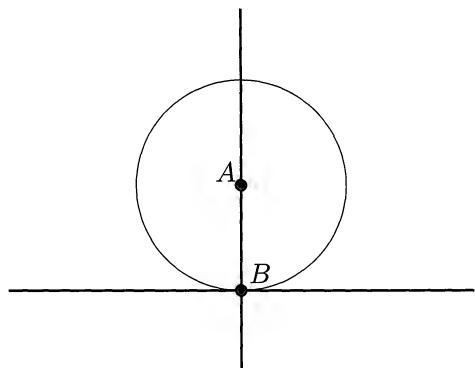
\includegraphics[width=0.42\textwidth]{figs/ch7s3-02.jpg}
\end{center}

——否则, 这个圆在第二个点 $C$ 处与 $\ell$ 相交 (无论 $A$ 是否在 $\ell$ 上):

\begin{center}
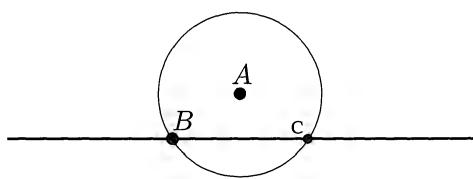
\includegraphics[width=0.42\textwidth]{figs/ch7s3-03.jpg}
\end{center}

一旦确定了 $C$, 过 $A$ 且垂直于 $\ell$ 的直线就可以通过连接分别以 $B$, $C$ 为圆心且经过 $C$, $B$ 的两个圆的两个交点 $D$, $E$ 而得到:

\begin{center}
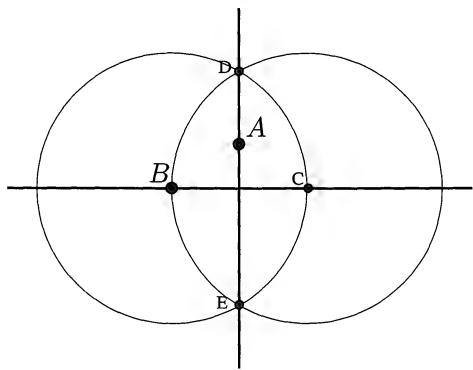
\includegraphics[width=0.42\textwidth]{figs/ch7s3-04.jpg}
\end{center}

对这个作图施用两次, 就得到过一点 $A$ 且平行于一条给定直线的直线:

\begin{center}
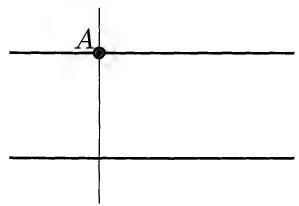
\includegraphics[width=0.42\textwidth]{figs/ch7s3-05.jpg}
\end{center}

这常常很方便.

对这些运算的审慎应用, 使我们能把一个笛卡儿坐标系引入画面. 从初始的两个点 $O$, $P$ 出发, 我们可以作出以 $O$ 为中心, 互相垂直的笛卡儿坐标轴, 并令 $P$ 标记 (比如说) ``$x$ 轴''上的点 $(1,0)$:

\begin{center}
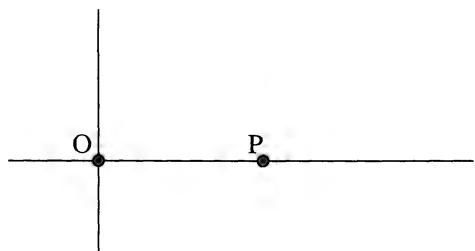
\includegraphics[width=0.5\textwidth]{figs/ch7s3-06.jpg}
\end{center}

而作一个点 $A=(x,y)$ 等价于作它在坐标轴上的投影 $X=(x,0)$, $Y=(0,y)$, 事实上又等价于作两个点 $X=(x,0)$ 与 $Y'=(y,0)$:

\begin{center}
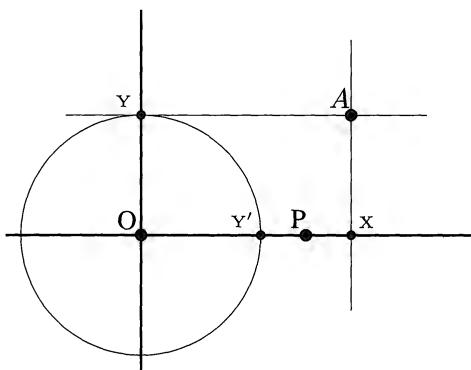
\includegraphics[width=0.5\textwidth]{figs/ch7s3-07.jpg}
\end{center}

\index{kegouzao@可构造(constructible)!jihetuxing@几何图形(geometric figures)}由此可见, 判定哪些图形能用直尺与圆规构造, 等价于判定哪些数可以作为一个可构造点的坐标来实现.

\index{kegouzao@可构造(constructible)!zhengduobianxing@正多边形(regular polygon)}\index{kegouzao@可构造(constructible)!shu@数(number)}\begin{definition}\label{def:constructible}
一个实数 $r$ 是\emph{可构造的}\index{ke gou zao@可构造的(constructible)}, 如果 (在上面取 $O=(0,0)$, $P=(1,0)$ 的意义下) 点 $(r,0)$ 能用直尺与圆规构造. 我们以 $\mathcal{C}_{\mathbb{R}}\subseteq\mathbb{R}$ 表示可构造实数之集.
\end{definition}

同样, 我们可以把实平面与 $\mathbb{C}$ 等同, 把 $O$ 放在 $0$, $P$ 放在 $1$, 并且说 $z=x+iy$ 是可构造的, 如果点 $(x,y)$ 能用直尺与圆规构造. 我们以 $\mathcal{C}_{\mathbb{C}}\subseteq\mathbb{C}$ 表示可构造复数之集. 总结前面的讨论, 我们证明了:

\begin{lemma}\label{lem:constructible-point}
点 $(x,y)$ 能用直尺与圆规构造, 当且仅当 $x+iy\in\mathcal{C}_{\mathbb{C}}$, 当且仅当 $x,y\in\mathcal{C}_{\mathbb{R}}$.
\end{lemma}

下一个显然的问题是这些可构造数之集携带何种结构, 这促使我们去看更多的几个基本直尺—圆规作图.

\begin{lemma}\label{lem:constructible-field}
可构造数之集 $\mathcal{C}_{\mathbb{R}}\subseteq\mathbb{R}$ 是 $\mathbb{R}$ 的一个子域. 类似地, $\mathcal{C}_{\mathbb{C}}$ 是 $\mathbb{C}$ 的一个子域, 而且事实上 $\mathcal{C}_{\mathbb{C}}=\mathcal{C}_{\mathbb{R}}(i)$.
\end{lemma}

\begin{proof}
$C_{\mathbb{R}}\subseteq\mathbb{R}$ 非空, 所以为了说明它是一个域, 我们只需证明它对减法以及除以一个非零可构造数封闭 (参见命题~II.\ref{prop:subgroup-criterion}).

读者将验证 $C_{\mathbb{R}}$ 对减法封闭 (习题~\ref{ex:construct-difference}). 为了看出 $C_{\mathbb{R}}$ 对除法封闭, 设 $a,b\in C_{\mathbb{R}}$, 且 $b\neq 0$. 由于按假设 $A=(0,a)$ 与 $B=(b,0)$ 可构造, 我们可以如上图\footnote{图中假设 $a>0$, $b>1$; 读者可以验证其他可能情形给出相同结论.} 那样, 把 $C$ 构造为过 $P=(1,0)$ 且平行于过 $A$, $B$ 的直线的直线与 $y$ 轴的交点:

\begin{center}
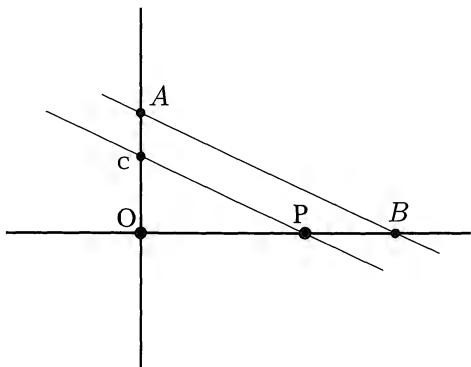
\includegraphics[width=0.42\textwidth]{figs/ch7s3-08.jpg}
\end{center}

由于三角形 $AOB$ 与 $COP$ 相似, 我们看到 $C=(0,a/b)$; 从而 $a/b$ 可构造.

$C_{\mathbb{C}}$ 是 $\mathbb{C}$ 的子域这一事实, 是 $C_{\mathbb{R}}$ 是域这一事实的直接推论, 其证明留给读者享受 (习题~\ref{ex:constructible-subfield-C}). 而 $\mathcal{C}_{\mathbb{C}}=\mathcal{C}_{\mathbb{R}}(i)$ 这个说法, 无非是重新表述了 ``$x+iy\in C_{\mathbb{C}}$ 当且仅当 $x$ 与 $y$ 都属于 $C_{\mathbb{R}}$'' 这一事实. \qed
\end{proof}

我们可以把 $C_{\mathbb{R}}$ 与 $C_{\mathbb{C}}$ 看作 $\mathbb{Q}$ 的扩张, 从而在直尺—圆规可构造性与域论之间架起一座桥: 如果我们能理解域扩张
\[
\mathbb{Q}\subseteq\mathcal{C}_{\mathbb{R}}\subseteq\mathcal{C}_{\mathbb{C}}
\]
就能理解几何图形的可构造性.

令人高兴的是, 我们能够理解这些扩张!

\subsection{可构造数与二次扩张}
\label{subsec:constructible-quadratic}

我们的目标是要证明下列关于 $C_{\mathbb{R}}$ (并从而立即给出 $C_{\mathbb{C}}$) 的惊人明确的描述.

\begin{theorem}\label{thm:constructible-quadratic}
设 $\gamma\in\mathbb{R}$. 则 $\gamma\in\mathcal{C}_{\mathbb{R}}$ 当且仅当存在实数 $\delta_1,\ldots,\delta_k$, 使得对所有 $j=1,\ldots,k$ 都有
\[
[\mathbb{Q}(\delta_1,\ldots,\delta_j):\mathbb{Q}(\delta_1,\ldots,\delta_{j-1})]=2
\]
并且 $\gamma\in\mathbb{Q}(\delta_1,\ldots,\delta_k)$.
\end{theorem}

换言之, $\gamma\in\mathbb{R}$ 可构造当且仅当它可以被放在 $\mathbb{Q}$ 之上的一串 (实) 二次扩张的顶层域中. 由于 $\mathcal{C}_{\mathbb{C}}=\mathcal{C}_{\mathbb{R}}(i)$, 同样的陈述对可构造复数也成立, 只需把 $i$ 列入 $\delta_j$ 的清单中 (或者干脆允许 $\delta_j$ 为复数; 参见习题~\ref{ex:complex-quadratic-constructible}).

这个定理的证明是尽可能显式具体的. 从一个给定的点 $(x,y)$ 的直尺—圆规作图出发, 人们可以得到陈述中所说的序列 $\delta_1,\ldots,\delta_k$, 使得 $x$ 与 $y$ 都属于扩张 $\mathbb{Q}(\delta_1,\ldots,\delta_k)$; 反过来, 从这个扩张中的任一元素 $\gamma$ 出发, 人们可以用直尺与圆规得到点 $(\gamma,0)$ 的一个明确的作图.

\begin{proof}
我们先在 ``几何到代数'' 的方向上论证. 一个由直尺—圆规作图得到的点, 直线, 圆的构型, 可以用这些点的坐标以及这些直线与圆的方程来描述. 假设在给定作图的某一步, 所有点的坐标以及所有直线与圆方程中的系数都属于某个域 $F$; 我们就说这个构型在 $F$ 上定义.

那么我们断言: 对下一步作出的每一个对象, 都存在一个实数 $\delta\in\mathbb{R}$, 它在 $F$ 上的次数至多为 $2$, 使得新的构型在 $F(\delta)$ 上定义. 定理的 ``仅当'' 部分由对作图步数归纳即得, 因为在开始时构型 (亦即点对 $O=(0,0)$, $P=(1,0)$) 在 $\mathbb{Q}$ 上定义.

验证我们的断言, 相当于对定义直尺—圆规作图的基本运算验证它. 读者将验证 (习题~\ref{ex:lines-circles-over-F}): 两条在 $F$ 上定义的直线的交点, 其坐标属于 $F$; 并且由坐标属于 $F$ 的点所决定的直线与圆, 都在 $F$ 上定义. 因此在所有这些情形中 $\delta=1$ 就够了.

对于一条直线 $\ell$ 与一个圆 $C$ 的交点, 假设 $\ell$ 不平行于 $y$ 轴 (否则论证完全类似), 并且它确实与 $C$ 相交; 令
\[
y=mx+r
\]
为 $\ell$ 的方程, 并令
\[
x^2+y^2+ax+by+c=0
\]
为 $C$ 的方程. 我们假设 $a,b,c,m,r\in F$. 那么 $\ell$ 与 $C$ 的交点的 $x$ 坐标是方程
\[
x^2+(mx+r)^2+ax+b(mx+r)+c=0
\]
的解. ``二次公式'' 表明这些坐标属于域 $F(\sqrt{D})$, 其中 $D$ 是这个多项式的判别式: 明确地,
\[
D=(2mr+bm+a)^2-4(m^2+1)(r^2+br+c),
\]
但这并不重要. 重要的是 $D\in F$; 从而 $\delta=\sqrt{D}$ 满足我们的要求.

对于两个 (不同的) 在 $F$ 上定义的圆的交点, 不需要任何新东西: 如果
\[
\left\{\begin{array}{l}
x^2+y^2+a_1x+b_1y+c_1=0,\\
x^2+y^2+a_2x+b_2y+c_2=0
\end{array}\right.
\]
是两个圆, 把两个方程相减表明它们的交点与一个圆和一条直线的交点重合:
\[
\left\{\begin{array}{l}
x^2+y^2+a_1x+b_1y+c_1=0,\\
(a_1-a_2)x+(b_1-b_2)y+(c_1-c_2)=0,
\end{array}\right.
\]
结论与前面的情形相同.

这就完成了定理 ``仅当'' 部分的验证.

为了证明具有如上陈述的扩张中的每一个元素都可构造, 再次用归纳论证: 只需证明如果 (i) $\delta\in\mathbb{R}$, (ii) $F$ 的所有元素都可构造, 并且 (iii) $r=\delta^2\in F$, 那么 $\delta$ 可构造 (注意, 为了构造一个在 $F$ 上次数为 $2$ 的元素, 只需构造极小多项式判别式的平方根). 因此, 我们所要证明的全部, 就是我们可以用直尺—圆规作图来 ``开平方''. 下面是这个图 (当 $r>1$ 时):

\begin{center}
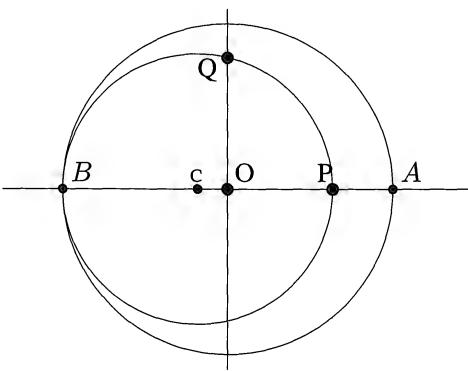
\includegraphics[width=0.42\textwidth]{figs/ch7s3-09.jpg}
\end{center}

如果 $A=(r,0)$ 可构造, 那么 $B=(-r,0)$ 也可构造; $C$ 是线段 $BP$ 的中点 (中点可构造, 见习题~\ref{ex:construct-midpoint}); 以 $C$ 为圆心且经过 $P$ 的圆与正 $y$ 轴相交于一点 $Q=(0,\delta)$, 而初等几何表明 $\delta^2=r$. 因此 $\delta$ 可构造, 这就完成了定理的证明.
\end{proof}

例如, 可以作出一个 $3^{\circ}$ 的角: 据称
\[
\cos 3^{\circ}=\frac{1}{8}(\sqrt{3}+1)\sqrt{5+\sqrt{5}}+\frac{1}{16}(\sqrt{6}-\sqrt{2})(\sqrt{5}-1),
\]
而这个式子表明
\[
\cos 3^{\circ}\in\mathbb{Q}(\sqrt{2},\sqrt{3},\sqrt{5})(\sqrt{5+\sqrt{5}});
\]
也就是说 (由定理~\ref{thm:constructible-quadratic}), $\cos 3^{\circ}$ 可构造. 当然, 一旦作出了 $A=(\cos\theta,0)$, 角 $\theta$ 也就作出了:

\begin{center}
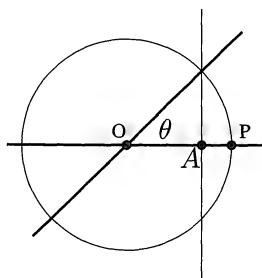
\includegraphics[width=0.42\textwidth]{figs/ch7s3-10.jpg}
\end{center}

下面是定理~\ref{thm:constructible-quadratic} 另一个 ``构造性'' 应用的例子.

\begin{example}\label{ex:pentagon-constructible}
正五边形可构造.

\begin{center}
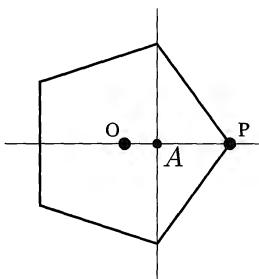
\includegraphics[width=0.42\textwidth]{figs/ch7s3-11.jpg}
\end{center}

确实, 只需作出点 $A=(\cos(2\pi/5),0)$, 而碰巧 $\gamma=\cos(2\pi/5)$ 满足
\begin{equation}
4\gamma^2+2\gamma-1=0.\tag{*}
\end{equation}
\index{huangjinbi@黄金比(golden ratio)}(事实上, $\gamma$ 是黄金分割比倒数的二分之一: $\gamma=\frac{\sqrt{5}-1}{4}$.) 由此可知 $\gamma\in\mathbb{Q}(\sqrt{5})$, 从而由定理~\ref{thm:constructible-quadratic} 它是可构造的. 事实上, 证明展示了如何构造 $\sqrt{5}$, 所以读者现在应当毫不费力地给出正五边形的一个直尺—圆规作图 (习题~\ref{ex:pentagon-construction}).
\end{example}

一旦我们把域论钻研得更透彻一些, 就会回到正多边形的作图问题 (参见 §\ref{subsec:constructible-ngons}). 顺便问一句, 人们是怎么猜到 $\gamma=\cos(2\pi/5)$ 应当满足恒等式 $(*)$ 的? 这借助一点复数运算很容易; 见习题~\ref{ex:verify-pentagon-relation}.

\subsection{著名的不可能性}
\label{subsec:famous-impossibilities}

定理~\ref{thm:constructible-quadratic} 通过下面的直接推论, 轻易地解决了 §\ref{subsec:straightedge-compass} 中提到的三个问题:

\begin{corollary}\label{cor:constructible-degree}
设 $\gamma\in\mathcal{C}_{\mathbb{C}}$ 是一个可构造数. 则 $[\mathbb{Q}(\gamma):\mathbb{Q}]$ 是 $2$ 的幂.
\end{corollary}

\begin{proof}
由引理~\ref{lem:constructible-field} 与定理~\ref{thm:constructible-quadratic}, 存在 $\delta_1,\ldots,\delta_k\in\mathbb{R}$ 使得
\[
\gamma\in\mathbb{Q}(\delta_1,\ldots,\delta_k,i),
\]
并且每个 $\delta_j$ 在 $\mathbb{Q}(\delta_1,\ldots,\delta_{j-1})$ 上的次数 $\leq 2$. 反复应用命题~\ref{prop:tower-degree} 表明
\[
[\mathbb{Q}(\delta_1,\ldots,\delta_k,i):\mathbb{Q}]
\]
是 $2$ 的幂, 而由于
\[
\mathbb{Q}\subseteq\mathbb{Q}(\gamma)\subseteq\mathbb{Q}(\delta_1,\ldots,\delta_k,i),
\]
结论由推论~\ref{cor:degree-divides} 推出.
\end{proof}

特别地, 可构造的实数也必须满足同样的条件.

考虑三等分角的问题. 我们知道可以作出一个 $60^{\circ}$ 的角 (这是作等边三角形的一个副产物). 作出一个 $20^{\circ}$ 的角等价于 (习题~\ref{ex:angle-constructible-cos}) 作出单位圆上辐角为 $\pi/9$ 的复数 $\gamma$:

\begin{center}
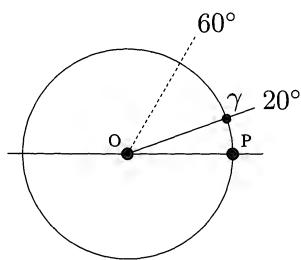
\includegraphics[width=0.42\textwidth]{figs/ch7s3-12.jpg}
\end{center}

现在 $\gamma^9=-1$; 也就是说, $\gamma$ 满足多项式
\[
t^9+1=(t^3+1)(t^6-t^3+1).
\]
它不满足 $t^3+1$; 因此它在 $\mathbb{Q}$ 上的极小多项式是
\[
t^6-t^3+1
\]
的一个因子. 然而, 这个多项式在 $\mathbb{Q}$ 上不可约 (作替换 $t\mapsto t-1$, 然后应用 Eisenstein 判别法), 所以
\[
[\mathbb{Q}(\gamma):\mathbb{Q}]=6.
\]
由推论~\ref{cor:constructible-degree}, $\gamma$ 不可构造. 因此存在可以作出但却不能被三等分的角.

类似地, 立方不能被倍: 因为那将蕴含 $\sqrt[3]{2}$ 的可构造性, 而它在 $\mathbb{Q}$ 上的次数为 $3$, 与推论~\ref{cor:constructible-degree} 矛盾.

化圆为方需要构造 $\sqrt{\pi}$. 但是如果 $\sqrt{\pi}$ 是代数数, 那么 $\pi$ 就会是代数数, 而它不是\erratumfootnote{根据官方勘误, 原书完善了化圆为方不可作的逻辑叙述: 化圆为方需构造 $\sqrt{\pi}$, 若 $\sqrt{\pi}$ 代数则 $\pi$ 代数, 从而导致矛盾 (原书此前曾简略为构造 $\pi$).} (尽管如我们提到过的, 这一事实的证明并不初等), 所以这也是不可能的.

作为另一个例子, 作正七边形相当于构造 $1$ 的一个 $7$ 次 (复) 单位根 $\zeta$:

\begin{center}
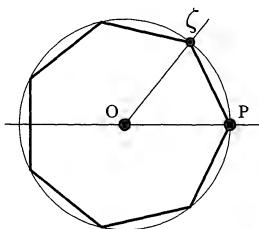
\includegraphics[width=0.42\textwidth]{figs/ch7s3-13.jpg}
\end{center}

依定义, $\zeta$ 满足
\[
t^7-1=(t-1)(t^6+t^5+\cdots+t+1);
\]
由于 $\zeta\neq 1$, $\zeta$ 必须满足分圆多项式 $t^6+\cdots+1$. 它在 $\mathbb{Q}$ 上不可约 (例~V.\ref{ex:cyclotomic-eisenstein}); 因此再次得到 $\zeta$ 在 $\mathbb{Q}$ 上的次数为 $6$, 而推论~\ref{cor:constructible-degree} 蕴含正七边形不能用直尺与圆规作出.

当然 ``$7$'' 并无特别之处: 如果 $p$ 是一个正素数, 则次数为 $p-1$ 的分圆多项式不可约 (还是例~V.\ref{ex:cyclotomic-eisenstein}); 从而
\[
[\mathbb{Q}(\zeta_p):\mathbb{Q}]=p-1,
\]
其中 $\zeta_p$ 是辐角为 $2\pi/p$ 的 $1$ 的复 $p$ 次单位根. 因此, 推论~\ref{cor:constructible-degree} 揭示: 如果 $p$ 是素数, 那么正 $p$ 边形可构造仅当 $p-1$ 是 $2$ 的幂. 这比初看上去限制更强, 因为若 $p=2^k+1$ 是素数, 则必有 $k$ 本身是 $2$ 的幂 (习题~\ref{ex:fermat-prime-power2}). 形如 $2^{2^{\ell}}+1$ 的素数称为 Fermat 素数:
\[
3,\ 5,\ 17,\ 257,\ 65537
\]
(``下一个'', $2^{32}+1=4294967297=641\cdot 6700417$, 不是素数; 事实上, 无人知道是否还有别的 Fermat 素数, 然而有些人猜想有无穷多个).

这些考察本身并不能告诉我们: 如果 $p$ 是 Fermat 素数, 那么正 $p$ 边形就能用直尺与圆规作出; 但它们确实告诉我们, 下一个要考虑的情形将是 $p=2^4+1=17$, 而碰巧 (正如 Gauss 在19岁时所指出的)
\[
\cos\frac{2\pi}{17}=\frac{\sqrt{17}-1+\sqrt{2}\sqrt{34+6\sqrt{17}+\sqrt{2}(\sqrt{17}-1)\sqrt{17-\sqrt{17}}-8\sqrt{2}\sqrt{17+\sqrt{17}}}+\sqrt{2}\sqrt{17-\sqrt{17}}}{16},
\]
因此 (由定理~\ref{thm:constructible-quadratic}) 正十七边形可用直尺与圆规作出. 正如我们已经宣布过的, 情况不久就会变得更加清晰, 使我们能够绕开繁重的三角学.

\subsection*{习题}
\phantomsection
\addcontentsline{toc}{subsection}{习题}

\begin{prob}\label{ex:construct-midpoint}
$\triangleright$ 证明: 若 $A$, $B$ 可构造, 则线段 $AB$ 的中点也可构造. 证明: 若两条直线 $\ell_1$, $\ell_2$ 可构造且不平行, 则平分 $\ell_1$, $\ell_2$ 所成角的两条直线也可构造. [§\ref{subsec:constructible-quadratic}]
\end{prob}

\begin{prob}\label{ex:construct-difference}
$\triangleright$ 证明: 若 $a$, $b$ 是可构造数, 则 $a-b$ 也是. [§\ref{subsec:straightedge-compass}]
\end{prob}

\begin{prob}\label{ex:construct-product}
找出两个实数之积的一个明确的直尺—圆规作图.
\end{prob}

\begin{prob}\label{ex:construct-square-triangle}
证明如何用直尺与圆规把三角形``方化'' (即作一个面积等于给定三角形面积的正方形).
\end{prob}

\begin{prob}\label{ex:lines-circles-over-F}
$\triangleright$ 设 $F$ 是 $\mathbb{R}$ 的一个子域.
\begin{itemize}
\item 设 $A=(x_A,y_A)$, $B=(x_B,y_B)$ 是 $\mathbb{R}^2$ 中两个点, 满足 $x_A,y_A,x_B,y_B\in F$. 证明过 $A$, $B$ 的直线在 $F$ 上定义 (亦即它容许一个系数属于 $F$ 的方程).
\item 证明以 $A$ 为圆心且经过 $B$ 的圆在 $F$ 上定义.
\item 设 $\ell_1$, $\ell_2$ 是 $\mathbb{R}^2$ 中两条不同的, 不平行的直线, 在 $F$ 上定义, 并设 $(x,y)=\ell_1\cap\ell_2$. 证明 $x,y\in F$.
\end{itemize}
[§\ref{subsec:constructible-quadratic}]
\end{prob}

\begin{prob}\label{ex:pentagon-construction}
$\triangleright$ 设计一种用直尺与圆规作正五边形的方法. [§\ref{subsec:constructible-quadratic}]
\end{prob}

\begin{prob}\label{ex:constructible-subfield-C}
$\triangleright$ 把 (实) 平面与 $\mathbb{C}$ 等同, 并把 $O$, $P$ 放在 $\mathbb{C}$ 的 $0$, $1$ 处. 设 $C_{\mathbb{C}}$ 是所有可构造点之集, 视为 $\mathbb{C}$ 的子集. 证明 $C_{\mathbb{C}}$ 是 $\mathbb{C}$ 的一个子域. [§\ref{subsec:straightedge-compass}]
\end{prob}

\begin{prob}\label{ex:constructible-modulus-arg}
设 $\delta\in\mathbb{C}$, $\delta\neq 0$, 并令 $\theta_{\delta}$ 为 $\delta$ 的辐角 (亦即过 $0$ 与 $\delta$ 的直线和实轴所夹的角). 证明 $\delta\in C_{\mathbb{C}}$ 当且仅当 $|\delta|$, $\cos\theta_{\delta}$, $\sin\theta_{\delta}$ 都是可构造实数.
\end{prob}

\begin{prob}\label{ex:complex-quadratic-constructible}
$\triangleright$ 设 $\gamma_1,\ldots,\gamma_k\in\mathcal{C}_{\mathbb{C}}$ 是可构造复数, 并设 $K$ 为域 $\mathbb{Q}(\gamma_1,\ldots,\gamma_k)\subseteq\mathcal{C}_{\mathbb{C}}$. 设 $\delta$ 是一个满足 $[K(\delta):K]=2$ 的复数. 证明 $\delta\in\mathcal{C}_{\mathbb{C}}$.

由此推出: 在 $\mathcal{C}_{\mathbb{C}}$ 上不存在二次的不可约多项式, 并且 $\mathcal{C}_{\mathbb{C}}$ 是具有此性质的最小的 $\mathbb{C}$ 的子域. [§\ref{subsec:constructible-quadratic}]
\end{prob}

\begin{prob}\label{ex:angle-constructible-cos}
$\triangleright$ 证明: 如果在任一可构造构型中两条直线形成一个角 $\theta$, 那么过 $O$ 且相对于直线 $OP$ 顺时针形成角 $\theta$ 的直线可构造.

由此推出: 一个角 $\theta$ 在平面中任何地方可构造, 当且仅当 $\cos\theta$ 可构造. [§\ref{subsec:famous-impossibilities}]
\end{prob}

\begin{prob}\label{ex:verify-pentagon-relation}
$\triangleright$ 验证 $\gamma=\cos(2\pi/5)$ 满足 §\ref{subsec:constructible-quadratic} 中给出的关系 $(*)$. (如果 $\sigma=\sin(2\pi/5)$, 注意 $z=\gamma+i\sigma$ 满足 $z^5-1$.) [§\ref{subsec:constructible-quadratic}]
\end{prob}

\begin{prob}\label{ex:angle-1-2-degree}
证明 $1^{\circ}$ 与 $2^{\circ}$ 的角不可构造. (提示: 根据我们目前所知, 你只需回想存在两个角之和的三角公式; 这些公式的确切形状并不重要.) 对哪些整数 $n$, 角 $n^{\circ}$ 可构造?
\end{prob}

\begin{prob}\label{ex:archimedes-trisection}
$\triangleright$ 证明在下图中 $\alpha=\frac{\theta}{3}$:

\begin{center}
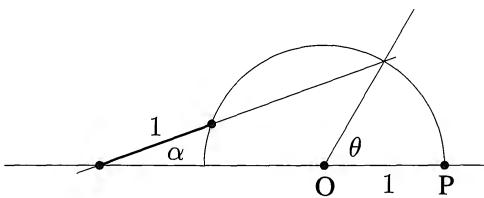
\includegraphics[width=0.42\textwidth]{figs/ch7s3-14.jpg}
\end{center}

这表明: 如果我们允许使用一把 ``标尺'' (亦即一把带标记的直尺), 那么角就可以被三等分 (这里, 这个作图在我们可以在区间上标记一个固定距离 $1$ 时有效). 显然, 这个作图阿基米德已经知道. [§\ref{subsec:straightedge-compass}]
\end{prob}

\begin{prob}\label{ex:nonconstructible-9gon}
证明正九边形不可构造.
\end{prob}

\begin{prob}\label{ex:fermat-prime-power2}
$\triangleright$ 证明: 如果 $2^k+1$ 是素数, 则 $k$ 是 $2$ 的幂. [§\ref{subsec:famous-impossibilities}]
\end{prob}

\section{域扩张, II}\label{sec:field-extensions-2}

是时候继续我们对各类域扩张的巡览了. 这里的关键词是分裂域、正规、可分.

\subsection{分裂域与正规扩张}\label{subsec:splitting-fields}

在 §\ref{subsec:algebraic-closure} 中我们构造了任意给定域 $k$ 的代数闭包 $\overline{k}$: $k[x]$ 中每个多项式都在 $\overline{k}[x]$ 中分裂为一次因式的乘积 (亦即``分裂''), 并且 $\overline{k}$ 是满足此性质的最小的 $k$ 的扩张.

下面是一个类似但温和得多的要求: 给定多项式的一个子集 $\mathcal{F}\subseteq k[x]$, 构造一个扩张 $k\subseteq F$, 使得 $\mathcal{F}$ 中每个多项式都在 $F$ 上分裂为一次因式的乘积, 并且要求 $F$ 在此意义下尽可能小. 此时我们称 $F$ 为 $\mathcal{F}$ 的分裂域. 实际上我们只对 $\mathcal{F}$ 为有限个多项式 $f_1(x),\ldots,f_r(x)$ 的情形感兴趣; 此时要求每个 $f_i(x)$ 在 $F$ 上分裂, 等价于要求乘积 $f_1(x)\cdots f_r(x)$ 在 $F$ 上分裂.

也就是说, 就我们的目的而言, 不妨假设 $\mathcal{F}$ 只由一个多项式 $f(x)\in k[x]$ 组成.

\begin{definition}\label{def:splitting-field}
设 $k$ 是一个域, $f(x)\in k[x]$ 是一个 $d$ 次多项式. $f(x)$ 在 $k$ 上的\emph{分裂域}是一个 $k$ 的扩张 $F$, 使得
\[
f(x)=c\prod_{i=1}^{d}(x-\alpha_i)
\]
在 $F[x]$ 中分裂, 并且进一步 $F=k(\alpha_1,\ldots,\alpha_d)$ 由 $f(x)$ 在 $F$ 中的根在 $k$ 上生成.
\end{definition}

需要注意的是, 分裂域的存在是显然的: 给定 $f(x)\in k[x]$, 子域 $F\subseteq\overline{k}$ (由 $f(x)$ 在 $\overline{k}$ 中的根在 $k$ 上生成) 即满足定义~\ref{def:splitting-field} 的要求. 但我们写定了``the splitting field'' (分裂域), 这是被下面的基本观察的唯一性部分所正当化的; 该观察还估出了这个扩张``有多大''.

\begin{lemma}\label{lem:splitting-field-unique}
设 $k$ 是一个域, $f(x)\in k[x]$. 则 $f(x)$ 在 $k$ 上的分裂域在同构意义下唯一, 并且 $[F:k]\leq(\deg f)!$.

事实上, 若 $\iota:k'\to k$ 是任意域同构, 且 $g(x)\in k'[x]$ 满足 $f(x)=\iota(g(x))$, 则 $\iota$ 可扩张为 $g(x)$ 在 $k'$ 上的任一分裂域到 $f(x)$ 在 $k$ 上的任一分裂域的同构.
\end{lemma}

\begin{proof}
\index{cishu@次数(degree)!bukefen@不可分(inseparable)}我们先显式构造一个分裂域, 并得到陈述中关于次数的界. 然后证明第二部分, 它蕴含在同构意义下的唯一性.

分裂域的构造以及对次数的界, 是我们在命题~V.\ref{prop:adjoin-root} 中得到的基本单扩张的一个简单应用. 归纳地论证: 假设对所有域和所有次数 $\leq(\deg f-1)$ 的多项式, 分裂域都已构造好, 并且界也已证得. 设 $q(t)$ 是 $f(t)$ 在 $k$ 上的任一不可约因子; 则
\[
k\subseteq F':=\frac{k[t]}{(q(t))}
\]
是一个次数为 $\deg q\leq\deg f$ 的扩张, 在其中 $q(x)$ (从而 $f(x)$) 有一个根 (即 $t$ 的陪集 $\alpha$), 因而有一次因子 $x-\alpha$. 多项式 $h(x):=f(x)/(x-\alpha)\in F'[x]$ 的次数为 $(\deg f-1)$; 因此 $h(x)$ 存在一个分裂域 $F$, 并且
\[
[F:F']\leq(\deg f-1)!.
\]
$f(x)$ 在 $F$ 上的因子是 $(x-\alpha)$ 和 $h(x)$ 的因子 (它们都是一次式); 由此推出 $F$ 是 $f(x)$ 的一个分裂域, 并且
\[
[F:k]=[F:F'][F':k]\leq(\deg f)(\deg f-1)!=(\deg f)!
\]
如前所述.

为证明同构 $\iota:k'\to k$ 能如陈述那样扩张为分裂域的同构, 设 $G$ 是 $g(x)$ 的一个分裂域, 并考虑复合 $k'\to k\subseteq\overline{k}$. 由于扩张 $k'\subseteq G$ 是代数的, 由引理~\ref{lem:embed-algebraic-ext} 存在 $G\to\overline{k}$ 的一个保 $k'$ 的扩张同态 $\iota:G\to\overline{k}$. 由于 $G$ 由 $g(x)$ 在 $G$ 中的根在 $k'$ 上生成, 我们有
\[
\iota(G)=k(\alpha_1,\dots,\alpha_d)\subseteq\overline{k},
\]
其中 $\alpha_i$ 是 $f(x)=\iota(g(x))$ 在 $\overline{k}$ 中的根. 因此 $L:=\iota(G)$ 与所选取的同构 $\iota$ 及分裂域 $G$ 无关. 将此观察分别用于给定的 $\iota$ 与恒等同构 $k\to k$, 即得陈述 (因为 $G$ 与 $F$ 都与 $L$ 同构).
\end{proof}

\begin{example}\label{ex:Qi-splitting}
按定义, $\mathbb{Q}(i)$ 是 $x^2+1$ 在 $\mathbb{Q}$ 上的分裂域, 而 $\mathbb{C}$ 是同一多项式在 $\mathbb{R}$ 上的分裂域.
\end{example}

\begin{example}\label{ex:x8-1-splitting}
$x^8-1$ 在 $\mathbb{Q}$ 上的分裂域 $F$ 由 $\zeta:=e^{2\pi i/8}$ 生成: 确实, $x^8-1$ 的根就是 $1$ 的全部 $8$ 次根, 而它们都是 $\zeta$ 的幂.
\begin{center}
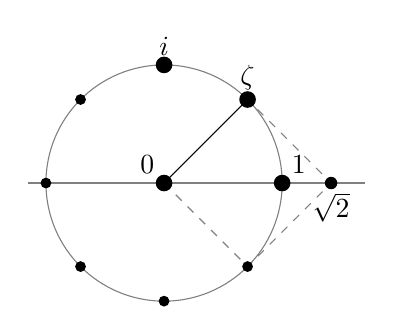
\begin{tikzpicture}[scale=1.5]
\draw[gray] (0,0) circle (1);
\draw[gray] (-1.15,0)--(1.7,0);
\draw (0,0)--(45:1);
\draw[dashed,gray] (0,0)--(-45:1)--({sqrt(2)},0)--(45:1);
\foreach \a in {0,45,...,315} {\fill (\a:1) circle (1.3pt);}
\fill (0,0) circle (2pt) node[above left] {$0$};
\fill (1,0) circle (2pt) node[above right] {$1$};
\fill (45:1) circle (2pt) node[above] {$\zeta$};
\fill (0,1) circle (2pt) node[above] {$i$};
\fill ({sqrt(2)},0) circle (1.5pt) node[below] {$\sqrt2$};
\end{tikzpicture}
\end{center}


实际上, $\zeta$ 是多项式 $x^4+1$ 的根, 而该多项式在 $\mathbb{Q}$ 上不可约; 因此 $F=\mathbb{Q}(\zeta)$ ``已经''是 $x^4+1$ 的分裂域. $F$ 在 $\mathbb{Q}$ 上的次数为
\[
[\mathbb{Q}(\zeta):\mathbb{Q}]=4,
\]
远小于引理~\ref{lem:splitting-field-unique} 给出的界 $8!$, $4!$.

为了更好理解这个分裂域, 注意到 $i=\zeta^2$ 属于 $F$, 并且 $\sqrt{2}=\zeta+\zeta^7$ 也属于 $F$; 于是 $F$ 包含 $\mathbb{Q}(i,\sqrt{2})$. 反过来, $\zeta=\frac{\sqrt{2}}{2}(1+i)\in\mathbb{Q}(i,\sqrt{2})$. 因此 $x^4+1$ 的分裂域 (亦即 $x^8-1$ 的分裂域) 就是 $\mathbb{Q}(i,\sqrt{2})$. 像我们在例~\ref{ex:sqrt2-sqrt3} 中对扩张 $\mathbb{Q}\subseteq\mathbb{Q}(i,\sqrt{2})$ 所做的那样分析, 可知其关于 $\mathbb{Q}$ 的自同构群是 $\mathbb{Z}/2\mathbb{Z}\times\mathbb{Z}/2\mathbb{Z}$.
\end{example}

\begin{example}\label{ex:x4-1-splitting}
主题的一个变体: $x^4-1$. 如果考虑的不是 $x^4+1$ 而是 $x^4-1$, 情形就不同了: 该多项式在 $\mathbb{Q}$ 上分解,
\[
x^4-1=(x-1)(x+1)(x^2+1),
\]
由此可知其分裂域与 $x^2+1$ 的分裂域相同, 即就是 $\mathbb{Q}(i)$.
\end{example}

\begin{example}\label{ex:x4+2-splitting}
主题的一个变体: $x^4+2$. 过于乐观的读者此刻或许期望, $x^4+1$ 与 $x^4-1$ 在 $\mathbb{Q}$ 上分裂域的不同, 仅仅源于前者在 $\mathbb{Q}$ 上不可约而后者可约. 这个例子会让任何这样的猜测胎死腹中. 沿用例~\ref{ex:x8-1-splitting} 的记号, $x^4+2$ 的根是
\[
\sqrt[4]{2}\,\zeta,\ \sqrt[4]{2}\,\zeta^3,\ \sqrt[4]{2}\,\zeta^5,\ \sqrt[4]{2}\,\zeta^7.
\]
因此, 以 $K=\mathbb{Q}(\sqrt[4]{2}\zeta,\sqrt[4]{2}\zeta^3,\sqrt[4]{2}\zeta^5,\sqrt[4]{2}\zeta^7)$ 记 $x^4+2$ 的分裂域, 有
\[
K\subseteq\mathbb{Q}(\zeta,\sqrt[4]{2})=\mathbb{Q}(i,\sqrt{2},\sqrt[4]{2})=\mathbb{Q}(i,\sqrt[4]{2}).
\]
另一方面, $\sqrt{2}=(\sqrt[4]{2}\zeta)^3/(\sqrt[4]{2}\zeta^3)\in K$; 从而 $i=(\sqrt[4]{2}\zeta)^2/\sqrt{2}\in K$; 从而 $\zeta=\frac{\sqrt{2}}{2}(1+i)\in K$; 从而 $\sqrt[4]{2}=(\sqrt[4]{2}\zeta)/\zeta\in K$. 于是 $\mathbb{Q}(i,\sqrt[4]{2})\subseteq K$, 结论便是 $x^4+2$ 的分裂域等于 $K=\mathbb{Q}(i,\sqrt[4]{2})$. 一个简单的次数计算 (习题~\ref{ex:aut-group-x4+2}) 表明 $[K:\mathbb{Q}]=8$, 特别地 $x^4+2$ 的分裂域当然不同构于 $x^4+1$ 的分裂域\erratumfootnote{根据官方勘误, 原书在此处完善了生成元包含关系的推理步骤与分裂域次数计算结论.}.

\index{duoxiangshi@多项式(polynomial)!zai UFD shangbukeyue@在 UFD 上不可约(irreducible over a UFD)}这样的例子总让我觉得域论必定相当神秘: 问题参数的看似无害的变化, 可能引起相应域扩张剧烈的改变. 从正面说, 这暗示域论确实是 (例如) 多项式研究中一件非常精确的工具.
\end{example}

\index{duoxiangshi@多项式(polynomial)!Laurent@Laurent}分裂域在后续故事中扮演着重要角色. 它们比初看起来还要特殊: 不仅分裂所给的多项式, 而且自动分裂任何``胆敢用一个根触碰它们''的不可约多项式. 这使分裂域成为正规扩张:

\begin{definition}\label{def:normal-extension}
一个域扩张 $k\subseteq F$ 是\emph{正规的}, 如果对每个不可约多项式 $f(x)\in k[x]$, $f(x)$ 在 $F$ 中有一个根当且仅当 $f(x)$ 在 $F$ 上分裂为一次因式的乘积.
\end{definition}

\begin{theorem}\label{thm:finite-normal-splitting}
一个域扩张 $k\subseteq F$ 是有限且正规的, 当且仅当 $F$ 是某个多项式 $f(x)\in k[x]$ 的分裂域.
\end{theorem}

\begin{proof}
假设 $k\subseteq F$ 有限且正规. 则 $F$ 有限生成: $F=k(\alpha_1,\ldots,\alpha_r)$, 其中每个 $\alpha_i$ 在 $k$ 上代数. 设 $p_i(x)$ 是 $\alpha_i$ 在 $k$ 上的极小多项式\erratumfootnote{根据官方勘误, 此处多项式不定元由 $t$ 统一记为 $x$ ($p_i(x)$ 与 $f(x)$).}. 由于 $F$ 在 $k$ 上正规, 每个 $p_i(x)$ 在 $F$ 上完全分裂, 从而 $f(x)=p_1(x)\cdots p_r(x)$ 也如此. 由此可知 $F$ 是 $f(x)$ 的分裂域.

反过来, 假设 $F$ 是某个多项式 $f(x)\in k[x]$ 的分裂域, 并设 $p(x)\in k[x]$ 是一个不可约多项式, 使得 $F$ 包含 $p(x)$ 的一个根 $\alpha$. 将 $F$ 视为代数闭包 $\overline{k}$ 的子域, 设 $\beta\in\overline{k}$ 是 $p(x)$ 的任一其他根; 我们将证明 $\beta\in F$. 这就证明了 $F$ 包含 $p(x)$ 的所有根, 从而 $k\subseteq F$ 正规, 并且由引理~\ref{lem:splitting-field-unique} 知 $k\subseteq F$ 有限.

由命题~\ref{prop:simple-ext-iso-lift}, 存在同构 $\iota:k(\alpha)\to k(\beta)$ 保 $k$ 上的恒等并将 $\alpha\mapsto\beta$. 我们还考虑子域 $F(\beta)\subseteq\overline{k}$, 视其为 $k(\beta)$ 的扩张. 把一切都放进一个图:

\begin{center}
\begin{tikzcd}[column sep=2.5em,row sep=1.4em]
& k(\alpha) \ar[dd,"\iota"] \ar[r,hook] & F \ar[r,hook] & \overline{k} \\
k \ar[ur,hook] \ar[dr,hook] & & & \\
& k(\beta) \ar[r,hook] & F(\beta) \ar[r,hook] & \overline{k}
\end{tikzcd}
\end{center}

(注意: 如果我们用恒等映射把右边的两个 $\overline{k}$ 连接起来, 相应的图并不交换: $\iota$ 把上行中的 $\alpha\in\overline{k}$ 送到下行中的 $\beta\in\overline{k}$.) 现在观察到, $F$ 可视为 $f(x)$ 在 $k(\alpha)$ 上的分裂域: 确实, 它包含 $f(x)$ 的所有根, 并且由这些根在 $k$ 上 (从而在 $k(\alpha)$ 上) 生成. 同理, $F(\beta)$ 是 $f(x)$ 在 $k(\beta)$ 上的分裂域. 由引理~\ref{lem:splitting-field-unique}, $\iota$ 可扩张为同构 $\iota':F\to F(\beta)$. 由于 $\iota$ 在 $k$ 上限制为恒等, $\iota'$ 是 $k$-向量空间的同构; 特别地, $\dim_k F=\dim_k F(\beta)$ (记住分裂域都是有限扩张).

现在考虑不同的 $k$-线性映射 $i:F\to F(\beta)$, 它简单地由在 $\overline{k}$ 中的包含给出:
\[
k\subseteq F\subseteq F(\beta)\subseteq\overline{k}.
\]
由于 $F$ 与 $F(\beta)$ 是同维数的有限维 $k$-向量空间, $i$ 也必须是同构. 换言之,
\[
[F(\beta):F]=1;
\]
即 $\beta\in F$, 如所求.
\end{proof}

\begin{remark}\label{rmk:normal-proof}
这个论证有点精巧. 沿用证明中的记号, 图
\begin{center}
\begin{tikzcd}[column sep=large,row sep=large]
k(\alpha) \ar[r,hook] \ar[d,"\iota"'] & F \ar[d,"\iota'"] \\
k(\beta) \ar[r,hook] & F(\beta)
\end{tikzcd}
\end{center}
是交换的, 而图
\begin{center}
\begin{tikzcd}[column sep=large,row sep=large]
k(\alpha) \ar[r,hook] \ar[d,"\iota"'] & F \ar[d,"i"] \\
k(\beta) \ar[r,hook] & F(\beta)
\end{tikzcd}
\end{center}
在 $\beta\neq\alpha$ 时不交换. 确实, $\iota$ 把 $\alpha$ 送到 $\beta$, 而 $i$ 把 $\alpha$ 送到 $\alpha$. 论证的要点是观察到: 若存在两个有限维向量空间 $V$, $W$ 之间的一个同构, 则每个单射线性映射 $V\to W$ 都必须是同构. 有限维性是得出结论所必需的; 参见习题~VI.\ref{ex:k[t]-injective-not-surjective}.
\end{remark}

\begin{example}\label{ex:normal-Qi-root4}
如果一个不可约多项式 $p(x)\in\mathbb{Q}[x]$ 的一个复根可以表示为 $i$ 与 $\sqrt[4]{2}$ 的带有理系数的多项式, 那么 $p(x)$ 的所有根也都可以同样用 $i$ 与 $\sqrt[4]{2}$ 表示. 确实, 我们已经验证 (例~\ref{ex:x4+2-splitting}) $\mathbb{Q}(i,\sqrt[4]{2})$ 是 $\mathbb{Q}$ 上的分裂域; 从而它是 $\mathbb{Q}$ 的正规扩张.
\end{example}

\subsection{可分多项式}\label{subsec:separable-polynomials}

我们的直觉或许会引导我们认为, 如果一个多项式分解为一次因式的乘积, 并且我们不是``故意''重复其中一个因子 (如 $(x-1)^2(x-2)$ 那样), 那么这些因子就会互异. 例如, 不可约多项式在代数闭包中分裂时, 其因子必然互异, 对吧? 错了.

\begin{example}\label{ex:xp-t-insep}
设 $p$ 是素数, 考虑 $\mathbb{F}_p$ 上的有理函数域 $\mathbb{F}_p(t)$. 则多项式
\[
x^p-t\in\mathbb{F}_p(t)[x]
\]
不可约: 由 Eisenstein 判别法它在 $\mathbb{F}_p[t][x]$ 中不可约 (因为 $(t)$ 在 $\mathbb{F}_p[t]$ 中是素理想), 从而由命题~V.\ref{prop:irreducible-over-field} 在 $\mathbb{F}_p(t)[x]$ 中不可约. 设 $u$ 是该多项式在某个 $L\supseteq\mathbb{F}_p(t)$ 中的根 (例如 $L$ 可以取 $\mathbb{F}_p(t)$ 的代数闭包, 或更温和地取该多项式的一个分裂域). 则 (习题~\ref{ex:frobenius-add})
\[
x^p-t=(x-u)^p
\]
在 $L[x]$ 中; 也就是说, $u$ 作为 $f(x)$ 的根具有重数 $p$.

换句话说, $u\in L$ 在 $\mathbb{F}_p(t)$ 上的极小多项式在 $u$ 处 $p$ 重为零, 对此我们无能为力: 没有比 $(x-u)^p=x^p-t$ 次数更小的 $(x-u)$ 的幂其系数落在 $\mathbb{F}_p(t)$ 中 (更小的幂会给出 $x^p-t$ 的一个非平凡因子, 而 $x^p-t$ 不可约).

我们一直觉得这个例子难以想象, 因为在特征 $0$ 中培养出的直觉; 并且如我们将看到的, 在特征 $0$ 中不可能出现这样的病态.
\end{example}

\begin{definition}\label{def:separable-poly}
设 $k$ 是一个域. 一个多项式 $f(x)\in k[x]$ 是\emph{可分的}, 如果它在自己的分裂域上没有重因子; $f(x)$ 是\emph{不可分的}, 如果它在自己的分裂域上有重因子.
\end{definition}

于是例~\ref{ex:xp-t-insep} 中的多项式 $x^p-t$ 是不可分的. 我们猜想这个术语反映了我们无法``分离''它的根: 它们像质子中的夸克一样抱成一团, 我们无法把它们拆开.

当然定义~\ref{def:separable-poly} 不依赖于所选取的分裂域, 因为这些分裂域在同构意义下唯一 (引理~\ref{lem:splitting-field-unique}). 事实上, 为了检测可分性, 我们可以使用任何一个使该多项式分裂为一次因式的域 (由习题~\ref{ex:splitting-field-hom}). 关于可分性的第一个 (有点令人惊讶的) 观察是, 我们其实不必离开 $f(x)$ 的系数域就能检测它. 这个事实用到了从微积分借来的一个概念: 对多项式
\[
f(x)=a_0+a_1x+a_2x^2+\dots+a_nx^n,
\]
我们以
\[
f'(x)=a_1+2a_2x+\dots+na_nx^{n-1}
\]
记其``导数''.

当然这是一个纯形式的运算; 在任意域上都不涉及极限过程. 尽管如此, 导数的一切预期性质都成立, 读者应当验证: 例如通常有 $(fg)'=f'g+fg'$.

\begin{lemma}\label{lem:separable-gcd}
设 $k$ 是一个域, $f(x)\in k[x]$. 则 $f(x)$ 可分当且仅当 $f(x)$ 与 $f'(x)$ 互素.
\end{lemma}

按定义, $f(x)$ 与 $f'(x)$ 互素恰好是它们的最大公因式为 $1$. 注意若 $k\subseteq F$, 则 $f(x)$ 与 $f'(x)$ 的最大公因式在 $k[x]$ 中与在 $F[x]$ 中是相同的: 例如因为它可以通过 Euclid 算法 (§V.\ref{subsec:euclidean-pid}) 计算, 而无论在计算在 $k[x]$ 中还是 $F[x]$ 中进行, 过程都完全一样.

\begin{proof}
先假设 $f(x)$ 不可分. 则 $f(x)$ 在某个分裂域 $F$ 中有重根; 即
\[
f(x)=(x-\alpha)^mg(x)
\]
对某个 $\alpha\in F$, $g(x)\in F[x]$, 且 $m\geq 2$. 于是
\[
f'(x)=m(x-\alpha)^{m-1}g(x)+(x-\alpha)^mg'(x),
\]
从而 $(x-\alpha)$ 是 $f(x)$ 与 $f'(x)$ 在 $F[x]$ 中的一个公因子. 因此 $\gcd(f(x),f'(x))\neq 1$ 在 $F[x]$ 中; 从而 $\gcd(f(x),f'(x))\neq 1$ 在 $k[x]$ 中; 即 $f(x)$, $f'(x)$ 不互素.

反过来, 假设 $\gcd(f(x),f'(x))\neq 1$, 于是 $f(x)$ 与 $f'(x)$ 在 $k$ 的代数闭包 $\overline{k}$ 中有一个公共的不可约因子 $(x-\alpha)$. 写 $f(x)=(x-\alpha)h(x)$; 我们有
\[
f'(x)=h(x)+(x-\alpha)h'(x),
\]
从而 $x-\alpha$ 整除 $h(x)$, 因为它整除 $f'(x)$. 但于是
\[
(x-\alpha)^2\mid f(x);
\]
故 $f(x)$ 不可分.
\end{proof}

例如, 例~\ref{ex:xp-t-insep} 中的多项式 $x^p-t$ 无须借助分裂域即可看出不可分: 在特征 $p$ 中 $x^p-t$ 的导数等于 $px^{p-1}=0$, 而 $\gcd(x^p-t,0)=x^p-t\neq 1$.

\index{bukefen@不可分(inseparable)}这个例子抓住了不可分性的一个关键特征:

\index{bukefen@不可分(inseparable)!chun@纯(purely)}\index{bukefen@不可分(inseparable)!duoxiangshi@多项式(polynomial)}\index{bukefen@不可分(inseparable)!kuozhangdeyuan@扩张的元(element of an extension)}\index{bukefen@不可分(inseparable)!cishu@次数(degree)}\begin{lemma}\label{lem:inseparable-deriv-zero}
设 $k$ 是一个域, $f(x)\in k[x]$ 是一个不可分的不可约多项式. 则 $f'(x)=0$.
\end{lemma}

\begin{proof}
由于 $f(x)$ 不可分, 由引理~\ref{lem:separable-gcd} 知 $f(x)$ 与 $f'(x)$ 有一个公共的不可约因子 $q(x)$; 但 $f(x)$ 自身不可约, 故 $q(x)$ 必与 $f(x)$ 相伴, 并且特别地其次数大于 $f'(x)$ 的次数 (若 $f'(x)\neq 0$). 由于 $q(x)\mid f'(x)$, 唯一的可能就是 $f'(x)=0$.
\end{proof}

\index{duoxiangshidedaoshu@多项式的导数(derivative of a polynomial)}这已经告诉我们, 不可约多项式在特征 $0$ 中必然可分: 在特征 $0$ 中, 一个非常数多项式的导数显然不可能为零. 事实上, 引理~\ref{lem:inseparable-deriv-zero} 给我们一幅关于不可分的不可约多项式必然形如怎样的精确图画. 如果
\[
f(x)=\sum_{i=0}^{n}a_ix^i
\]
不可约且不可分, 则域的特征必为正素数 $p$, 并且由引理~\ref{lem:inseparable-deriv-zero} 必有
\[
f'(x)=\sum_{i=0}^{n}ia_ix^{i-1}=0;
\]
即对所有 $i$ 有 $ia_i=0$. 现在若 $i$ 是 $p$ 的倍数, 则 $ia_i=0$ 自动成立; 而它对一切不是 $p$ 的倍数的指标 $i$ 推出 $a_i=0$. 因此 $f(x)$ 中唯一可能非零的系数, 是那些对应于 $p$ 的倍数指标的:
\[
f(x)=a_0+a_px^p+a_{2p}x^{2p}+\ldots;
\]
于是 $f(x)$ 实际上必须是一个 $x^p$ 的多项式. (读者将通过完成习题~\ref{ex:inseparable-degree} 及其后续而进一步细化这幅图画.)

这引导我们得到一个把可分性与我们尚未遇到的一类域联系起来的精确结果.

\begin{definition}\label{def:frobenius}
设 $k$ 是特征 $p>0$ 的域. \emph{Frobenius 同态}是映射 $k\to k$, 定义为 $x\mapsto x^p$.
\end{definition}

Frobenius 同态乍看不像一个环同态, 但它确实是 (习题~\ref{ex:frobenius-add}). 它必然单射, 正如每个非平凡的域同态那样; 但它未必满射.

\begin{definition}\label{def:perfect}
一个域 $k$ 是\emph{完全的}, 如果 $\Char k=0$, 或者 $\Char k>0$ 且 Frobenius 同态是满射.
\end{definition}

\begin{proposition}\label{prop:perfect-sep}
设 $k$ 是一个域. 则 $k$ 是完全的当且仅当 $k[x]$ 中所有不可约多项式都可分.
\end{proposition}

\begin{proof}
我们将证明完全域上的不可约多项式可分, 把另一个方向留给读者 (习题~\ref{ex:not-perfect-insep}).

我们已经注意到, 特征为零的域上的不可约多项式可分. 在正特征 $p$ 中, 我们观察到, 一个不可分的不可约多项式必形如
\[
f(x)=\sum_{i=0}^{m}a_i\cdot(x^p)^i.
\]
由于 Frobenius 是满射, 存在 $b_i$ 使得 $b_i^p=a_i$. 于是
\[
f(x)=\sum_{i=0}^{m}b_i^p(x^p)^i=\sum_{i=0}^{m}(b_ix^i)^p=\left(\sum_{i=0}^{m}b_ix^i\right)^p=g(x)^p,
\]
其中 $g(x)=\sum b_ix^i$, 并记住 Frobenius 映射是一个同态. 但这与 $f(x)$ 的不可约性矛盾, 故不存在这样的多项式.
\end{proof}

\begin{corollary}\label{cor:finite-fields-perfect}
\index{youxianyu@有限域(finite field)}有限域是完全的. 从而, 在有限域上, 不可约多项式都可分.
\end{corollary}

\begin{proof}
Frobenius 映射是单射 (因为它是域的同态), 从而在有限域上由鸽笼原理它是满射. 因此有限域是完全的, 而陈述的第二部分由命题~\ref{prop:perfect-sep} 推出. \qed
\end{proof}

读者现在明白我们为何在例~\ref{ex:xp-t-insep} 中选择那个有点不寻常的域 $\mathbb{F}_p(t)$ 了: 我们需要一个正特征的域, 但是在 $F_p$ 上由推论~\ref{cor:finite-fields-perfect} 找不到任何不可分的不可约多项式的例子; 为了构造一个例子, 我们必须放大这个域使其无限, 并且塞进一个元素 (即 $t$), 它对它没有 $p$ 次根, 亦即不在 Frobenius 的像中.

\subsection{可分扩张与在代数闭包中的嵌入}\label{subsec:separable-extensions-embeddings}

上一小节考察的术语可以推广到域扩张的语言中. 如果 $k\subseteq F$ 是一个扩张且 $\alpha\in F$ 在 $k$ 上代数, 我们说 $\alpha$ 在 $k$ 上\emph{可分}, 如果 $\alpha$ 在 $k$ 上的极小多项式可分; 否则 $\alpha$ \emph{不可分}.

\begin{definition}\label{def:separable-extension}
一个代数域扩张 $k\subseteq F$ 是\emph{可分的}, 如果每个 $\alpha\in F$ 都在 $k$ 上可分.
\end{definition}

用这个术语, 命题~\ref{prop:perfect-sep} 可以重述为以下更唬人的形式:

\begin{proposition}\label{prop:perfect-sep-ext}
一个域 $k$ 是完全的, 当且仅当 $k$ 的每个代数扩张都可分.
\end{proposition}

特别地, $\mathbb{Q}$ (或任意特征为零的域) 的代数扩张, 以及每个有限域的代数扩张, 必然可分.

可分性条件极其方便, 并且我们此后实质上采用它: 我们将认真考虑的所有扩张都是可分的. 可分扩张的一个方便的特性, 是以下对可分性条件的另一种刻画.

我们已经看到 (引理~\ref{lem:embed-algebraic-ext}) 每个代数扩张 $k\subseteq F$ 都可嵌入一个代数闭包 $k\subseteq\overline{k}$, 并且我们指出这一般可以用许多不同的方式做到. 如果是有限的, 把 $F\to\overline{k}$ 中保 $k$ 上恒等的不同同态的个数记为
\[
[F:k]_s.
\]

\begin{definition}\label{def:separable-degree}
这就是 $F$ 在 $k$ 上的\emph{可分次数}.
\end{definition}

显然这个数与所选取的代数闭包 $k\subseteq\overline{k}$ 无关. 它与可分性有什么关系呢?

\begin{lemma}\label{lem:simple-sep-degree}
设 $k\subseteq k(\alpha)$ 是一个单代数扩张. 则 $[k(\alpha):k]_s$ 等于 $\alpha$ 的极小多项式在 $\overline{k}$ 中不同根的个数. 特别地, $[k(\alpha):k]_s\leq[k(\alpha):k]$, 并且等号成立当且仅当 $\alpha$ 在 $k$ 上可分.
\end{lemma}

\begin{proof}
证明实质上是 (并且不是巧合地) 推论~\ref{cor:autk-count} 证明的重述. 把每个保 $\mathrm{id}_k$ 的 $\iota:k(\alpha)\to\overline{k}$ 与其像 $\iota(\alpha)$ 对应, 后者必是 $\alpha$ 的极小多项式的根. 这个对应是单射, 因为 $\iota(\alpha)$ 决定了 $\iota$ (由于 $\iota$ 扩充 $k$ 上的恒等). 为见其满射, 设 $\beta\in\overline{k}$ 是任一其他根, 并考虑扩张 $k(\beta)\subseteq\overline{k}$; 由命题~\ref{prop:simple-ext-iso-lift} 存在同构 $k(\alpha)\to k(\beta)$ 把 $\alpha$ 送到 $\beta$, 再与嵌入 $k(\beta)\subseteq\overline{k}$ 复合即定义出相应的 $\iota$, 如所求.
\end{proof}

\index{cishu@次数(degree)!kefen@可分(separable)}于是, 对单扩张而言, ``可分次数''确实检测可分性. 进一步, 它对连续扩张是乘法的:

\begin{lemma}\label{lem:sep-degree-tower}
设 $k\subseteq E\subseteq F$ 是代数扩张. 则 $[F:k]_s$ 有限当且仅当 $[F:E]_s$, $[E:k]_s$ 都有限, 并且此时
\[
[F:k]_s=[F:E]_s[E:k]_s.
\]
\end{lemma}

\begin{proof}
$E$ 到 $\overline{k}$ 的不同嵌入的不同延拓, 由引理~\ref{lem:embed-algebraic-ext} 给出 $F$ 到 $\overline{k}$ 的不同嵌入; 而 $F$ 到 $\overline{E}=\overline{k}$ 中保 $E$ 上恒等的嵌入, 当然也保 $k$ 上的恒等. 因此, 若 $[F:E]_s$, $[E:k]_s$ 中有一个无限, 则 $[F:k]_s$ 也无限.

对反向蕴含, 只需证明所陈述的次数公式. 但每个保 $k$ 上恒等的嵌入 $F\subseteq\overline{k}$ 都可由两步得到: 先把恒等扩张为嵌入 $E\subseteq\overline{k}$, 这有 $[E:k]_s$ 种做法; 再把所选取的嵌入 $E\subseteq\overline{k}=\overline{E}$ 扩张为嵌入 $F\subseteq\overline{E}=\overline{k}$, 这有 $[F:E]_s$ 种做法. 恰好有 $[F:E]_s[E:k]_s$ 种做法, 如陈述.
\end{proof}

引理~\ref{lem:simple-sep-degree} 与引理~\ref{lem:sep-degree-tower} 使我们能把有限扩张的可分性完全用代数闭包中嵌入的计数来重述:

\begin{proposition}\label{prop:finite-sep-degree}
设 $k\subseteq F$ 是一个有限扩张. 则 $[F:k]_s\leq[F:k]$, 并且以下等价:

(i) $F=k(\alpha_1,\ldots,\alpha_r)$, 其中每个 $\alpha_i$ 在 $k$ 上可分;

(ii) $k\subseteq F$ 可分;

(iii) $[F:k]_s=[F:k]$.
\end{proposition}

\begin{proof}
由于 $F$ 在 $k$ 上有限, 它有限生成. 设 $F=k(\alpha_1,\ldots,\alpha_r)$. 则利用引理~\ref{lem:sep-degree-tower}, 引理~\ref{lem:simple-sep-degree}, 以及命题~\ref{prop:tower-degree},
\[
\begin{array}{r l}
[F:k]_s & =[k(\alpha_1,\ldots,\alpha_{r-1})(\alpha_r):k(\alpha_1,\ldots,\alpha_{r-1})]_s\cdots[k(\alpha_1):k]_s \\
& \leq [k(\alpha_1,\ldots,\alpha_{r-1})(\alpha_r):k(\alpha_1,\ldots,\alpha_{r-1})]\cdots[k(\alpha_1):k] \\
& =[F:k].
\end{array}
\]
这证明了所陈述的不等式.

(i)$\Longrightarrow$(iii): 若每个 $\alpha_i$ 在 $k$ 上可分, 则它在域 $k(\alpha_1,\ldots,\alpha_{i-1})$ 上也可分 (习题~\ref{ex:separable-over-intermediate}), 故由引理~\ref{lem:simple-sep-degree} 不等式取等号.

(iii)$\Longrightarrow$(ii): 假设 $[F:k]_s=[F:k]$, 并设 $\alpha\in F$. 我们有 $k\subseteq k(\alpha)\subseteq F$; 从而由引理~\ref{lem:sep-degree-tower}
\[
[F:k(\alpha)]_s[k(\alpha):k]_s=[F:k]_s=[F:k]=[F:k(\alpha)][k(\alpha):k].
\]
\index{fenci@分次(graded)}由于两个可分次数都小于等于各自的普通次数, 这个等式推出
\[
[k(\alpha):k]_s=[k(\alpha):k],
\]
由引理~\ref{lem:simple-sep-degree} 即证 $\alpha$ 可分. 因此扩张 $k\subseteq F$ 按定义~\ref{def:separable-extension} 可分.

(ii)$\Longrightarrow$(i) 由定义~\ref{def:separable-extension} 立得, 因为有限扩张有限生成.
\end{proof}

例如, 若 $\alpha$ 在 $k$ 上可分, 则每个 $\beta\in k(\alpha)$ 都可分. 这单从定义看会显得相当神秘: 为什么 $\alpha$ 的极小多项式在 $\overline{k}$ 中有互异的根, 就能推出 $\beta$ 的极小多项式也如此? 它确实能, 凭借命题~\ref{prop:finite-sep-degree}.

\begin{remark}\label{rmk:sep-degree-divides}
虽然我们只证明了 $[F:k]_s\leq[F:k]$, 其实还可以证明 $[F:k]_s$ 整除 $[F:k]$: 事实上, $[F:k]_s$ 是某个中间域 $F_{\mathrm{sep}}$ 在 $k$ 上的次数. 勤勉的读者将在习题~\ref{ex:inseparable-degree-props} 中证明这一点.\index[sym1]{17@$F_{\mathrm{sep}}$}
\end{remark}

\subsection*{习题}
\phantomsection
\addcontentsline{toc}{subsection}{习题}

\begin{prob}\label{ex:splitting-field-hom}
$\triangleright$ 设 $k$ 是域, $f(x)\in k[x]$, 并设 $F$ 是 $f(x)$ 在 $k$ 上的分裂域. 设 $k\subseteq K$ 是一个扩张, 使得 $f(x)$ 在 $K$ 上分裂为一次因式的乘积. 证明存在同态 $F\to K$ 保 $k$ 上的恒等. [§\ref{subsec:splitting-fields}]
\end{prob}

\begin{prob}\label{ex:splitting-x6+x3+1}
描述 $x^6+x^3+1$ 在 $\mathbb{Q}$ 上的分裂域. 对 $x^4+4$ 做同样的事.
\end{prob}

\begin{prob}\label{ex:aut-group-x4+2}
$\triangleright$ 求 $x^4+2$ 在 $\mathbb{Q}$ 上的分裂域的自同构群的阶 (参见例~\ref{ex:x4+2-splitting})\erratumfootnote{根据官方勘误, 此题编号与对应的例交叉引用核对一致 (cf. Example 4.6).}. [§\ref{subsec:splitting-fields}]
\end{prob}

\begin{prob}\label{ex:Q-root4-not-splitting}
证明域 $\mathbb{Q}(\sqrt[4]{2})$ 不是任何 $\mathbb{Q}$ 上多项式的分裂域.
\end{prob}

\begin{prob}\label{ex:splitting-of-factor}
$\triangleright$ 设 $F$ 是多项式 $f(x)\in k[x]$ 的一个分裂域, 并设 $g(x)\in k[x]$ 是 $f(x)$ 的一个因子. 证明存在唯一的中间域 $k\subseteq G\subseteq F$ 使得 $k\subseteq G$ 是 $g(x)$ 的分裂域\erratumfootnote{根据官方勘误, 原题陈述严密化为: ``存在唯一的中间域 $k\subseteq G\subseteq F$ 使得 $k\subseteq G$ 是 $g(x)$ 的分裂域 (there is a unique intermediate field $k\subseteq G\subseteq F$ such that $k\subseteq G$ is a splitting field for $g(x)$)''.}. [\S\ref{subsec:finite-fields}]
\end{prob}

\begin{prob}\label{ex:intersection-composite-splitting}
设 $k\subseteq F_1$, $k\subseteq F_2$ 是两个有限扩张, 视为嵌入 $k$ 的代数闭包 $\overline{k}$ 中. 假设 $F_1$ 与 $F_2$ 都是 $k[x]$ 中多项式的分裂域. 证明交 $F_1\cap F_2$ 与复合 $F_1F_2$ ($\overline{k}$ 中包含 $F_1$ 与 $F_2$ 的最小子域) 也都是 $k$ 上的分裂域. (定理~\ref{thm:finite-normal-splitting} 大概会有帮助.)
\end{prob}

\begin{prob}\label{ex:simple-normal-aut}
$\triangleright$ 设 $k\subseteq F=k(\alpha)$ 是一个单代数扩张. 证明 $F$ 在 $k$ 上正规, 当且仅当对每个代数扩张 $F\subseteq K$ 和每个 $\sigma\in\Aut_k(K)$, 都有 $\sigma(F)=F$. [\S\ref{subsec:galois-correspondence}]
\end{prob}

\begin{prob}\label{ex:frobenius-add}
$\triangleright$ 设 $p$ 是素数, $k$ 是特征 $p>0$ 的域. 对 $a,b\in k$\erratumfootnote{根据官方勘误, 特征明确标明为 $p>0$, 元素所属域由大写 $K$ 修正为小写 $k$ ($a,b\in k$).}, 证明\footnote{这就是所谓``菜鸟之梦''; 它在任意特征 $p$ 的交换环中都成立, 由二项式定理以及中间二项式系数 $\binom{p}{k}$ 对 $0<k<p$ 均被 $p$ 整除.} $(a+b)^p=a^p+b^p$. [§\ref{subsec:separable-polynomials}, §\ref{subsec:finite-fields}, §\ref{subsec:cyclotomic}]
\end{prob}

\begin{prob}\label{ex:derivative-product}
利用 §\ref{subsec:separable-polynomials} 中给出的``导数''概念, 证明对所有多项式 $f$, $g$ 有 $(fg)'=f'g+fg'$.
\end{prob}

\begin{prob}\label{ex:char-p-not-divide-sep}
设 $k\subseteq F$ 是特征 $p>0$ 的有限扩张. 假设 $p$ 不整除 $[F:k]$. 证明 $k\subseteq F$ 可分.
\end{prob}

\begin{prob}\label{ex:frobenius-Fp-identity}
$\triangleright$ 设 $p$ 是素数. 证明 $F_p$ 上的 Frobenius 同态是恒等映射. (提示: Fermat 小定理.) [\S\ref{subsec:finite-fields}]
\end{prob}

\begin{prob}\label{ex:not-perfect-insep}
$\triangleright$ 设 $k$ 是域, 并假设 $k$ 不完全. 证明 $k[x]$ 中存在不可分的不可约多项式. (若 $\Char k=p$ 且 $u\in k$, 则 $x^p-u$ 在 $\overline{k}$ 中有多少个根?) [§\ref{subsec:separable-polynomials}]
\end{prob}

\begin{prob}\label{ex:inseparable-degree}
$\triangleright$ 设 $k$ 是正特征 $p$ 的域, $f(x)$ 是一个不可约多项式. 证明存在整数 $d$ 和一个可分不可约多项式 $f_{\mathrm{sep}}(x)$, 使得
\[
f(x)=f_{\mathrm{sep}}(x^{p^d}).
\]
数 $p^d$ 称为 $f(x)$ 的\emph{不可分次数}. 若 $f(x)$ 是代数元 $\alpha$ 的极小多项式, 则 $\alpha$ 的不可分次数定义为 $f(x)$ 的不可分次数. 证明 $\alpha$ 不可分当且仅当其不可分次数 $\geq p$.

要牢记的图画如下: $\alpha$ 的极小多项式 $f(x)$ 的根分布成 $\deg f_{\mathrm{sep}}$ 个``团'', 每个团收集若干重合的根, 其个数等于 $\alpha$ 的不可分次数. 若只有一个团 (即 $f(x)$ 的所有根重合), 我们说 $\alpha$ 是\emph{纯不可分的} (参见习题~\ref{ex:purely-inseparable}). [§\ref{subsec:separable-polynomials}, \ref{ex:purely-inseparable}, \ref{ex:inseparable-degree-props}]
\end{prob}

\begin{prob}\label{ex:purely-inseparable}
$\neg$ 设 $k\subseteq F$ 是正特征 $p$ 的代数扩张. 元素 $\alpha\in F$ 在 $k$ 上\emph{纯不可分}, 如果存在某个 $d\geq 0$\footnote{这个术语并不完全一致: $k$ 中的元素也称为纯不可分的, 尽管它们并不是不可分的.} 有 $\alpha^{p^d}\in k$. 该扩张称为\emph{纯不可分的}, 如果每个 $\alpha\in F$ 都在 $k$ 上纯不可分.

证明 $\alpha$ 纯不可分当且仅当 $[k(\alpha):k]_s=1$, 当且仅当它的次数等于它的不可分次数 (习题~\ref{ex:inseparable-degree}). [\ref{ex:inseparable-degree}, \ref{ex:Fsep-purely-insep}]
\end{prob}

\begin{prob}\label{ex:separable-over-intermediate}
$\triangleright$ 设 $k\subseteq F$ 是代数扩张, 并设 $\alpha\in F$ 在 $k$ 上可分. 对每个中间域 $k\subseteq E\subseteq F$, 证明 $\alpha$ 在 $E$ 上可分. [§\ref{subsec:separable-extensions-embeddings}]
\end{prob}

\begin{prob}\label{ex:sep-closure}
$\neg$ 设 $k\subseteq F$ 是代数扩张. 证明若 $k\subseteq E\subseteq F$ 是代数域扩张, 且 $k\subseteq E$ 可分, 则只要 $\alpha\in F$ 在 $E$ 上可分, 就有 $k\subseteq E(\alpha)$ 是可分扩张. (归约到有限扩张的情形.)

推出 $F$ 中在 $k$ 上可分的元素构成一个中间域 $F_{\mathrm{sep}}$, 使得每个 $\alpha\in F$, $\alpha\notin F_{\mathrm{sep}}$ 都在 $F_{\mathrm{sep}}$ 上不可分.

对 $F=\overline{k}$, $\overline{k}_{\mathrm{sep}}$ 称为 $k$ 的\emph{可分闭包}. [\ref{ex:Fsep-purely-insep}, \ref{ex:inseparable-degree-props}]
\end{prob}

\begin{prob}\label{ex:Fsep-purely-insep}
$\neg$ 设 $k\subseteq F$ 是正特征的代数扩张. 沿用习题~\ref{ex:purely-inseparable} 与习题~\ref{ex:sep-closure} 的记号, 证明扩张 $F_{\mathrm{sep}}\subseteq F$ 纯不可分. 证明一个扩张 $k\subseteq F$ 纯不可分当且仅当 $F_{\mathrm{sep}}=k$. [\ref{ex:inseparable-degree-props}]
\end{prob}

\begin{prob}\label{ex:inseparable-degree-props}
$\triangleright$ 设 $k\subseteq F$ 是正特征的有限扩张. 定义不可分次数 $[F:k]_i$ 为商 $[F:k]/[F:k]_s$.

\begin{itemize}
\item[(a)] 证明 $[k(\alpha):k]_i$ 等于习题~\ref{ex:inseparable-degree} 中定义的 $\alpha$ 的不可分次数.
\item[(b)] 证明不可分次数是乘法的: 若 $k\subseteq E\subseteq F$ 是有限扩张, 则 $[F:k]_i=[F:E]_i[E:k]_i$.
\item[(c)] 证明一个有限扩张纯不可分当且仅当它的不可分次数等于它的次数.
\item[(d)] 沿用习题~\ref{ex:sep-closure} 的记号, 证明 $[F:k]_s=[F_{\mathrm{sep}}:k]$ 且 $[F:k]_i=[F:F_{\mathrm{sep}}]$. (利用习题~\ref{ex:Fsep-purely-insep}.)
\end{itemize}

特别地, $[F:k]_s$ 整除 $[F:k]$; 不可分次数 $[F:k]_i$ 是一个整数. [§\ref{subsec:separable-extensions-embeddings}]
\end{prob}

\begin{prob}\label{ex:norm-trace-embeddings}
$\neg$ 设 $k\subseteq F$ 是有限可分扩张, 并设 $\iota_1,\ldots,\iota_d$ 是 $F$ 到 $\overline{k}$ 中保 $\mathrm{id}_k$ 的不同嵌入. 对 $\alpha\in F$, 证明范数 $N_{k\subseteq F}(\alpha)$ (参见习题~\ref{ex:norm-alpha}) 等于 $\prod_{i=1}^{d}\iota_i(\alpha)$, 而其迹 $\tr_{k\subseteq F}(\alpha)$ (习题~\ref{ex:trace-alpha}) 等于 $\sum_{i=1}^{d}\iota_i(\alpha)$. (提示: 习题~\ref{ex:trace-norm-simple} 与习题~\ref{ex:trace-norm-tower}.) [\ref{lem:simple-sep-degree}, \ref{lem:sep-degree-tower}, \ref{ex:norm-trace-product}]
\end{prob}

\begin{prob}\label{ex:norm-trace-aut}
$\neg$ 设 $k\subseteq F$ 是有限可分扩张, 并设 $\alpha\in F$. 证明对所有 $\sigma\in\Aut_k(F)$, 有 $N_{k\subseteq F}(\alpha/\sigma(\alpha))=1$ 且 $\tr_{k\subseteq F}(\alpha-\sigma(\alpha))=0$. [\ref{ex:hilbert90-multiplicative}, \ref{ex:hilbert90-additive}]
\end{prob}

\begin{prob}\label{ex:norm-trace-tower}
$\neg$ 设 $k\subseteq E\subseteq F$ 是有限可分扩张, 并设 $\alpha\in F$. 证明
\[
N_{k\subseteq F}(\alpha)=N_{k\subseteq E}(N_{E\subseteq F}(\alpha))\quad\text{且}\quad\tr_{k\subseteq F}(\alpha)=\tr_{k\subseteq E}(\tr_{E\subseteq F}(\alpha)).
\]
(提示: 利用习题~\ref{ex:norm-trace-embeddings}: 若 $d=[E:k]$ 且 $e=[F:E]$, 则 $F$ 到 $\overline{k}$ 中保 $\mathrm{id}_k$ 的 $de$ 个嵌入, 按它们在 $E$ 上的限制分成 $d$ 组, 每组 $e$ 个.)

这个范数与迹的``传递性''把习题~\ref{ex:trace-norm-tower} 的结果推广到了可分扩张. 可分性的限制其实不必要; 参见习题~\ref{ex:norm-trace-gen}. [\ref{ex:norm-trace-gen}]
\end{prob}

\begin{prob}\label{ex:norm-trace-gen}
把习题~\ref{ex:norm-trace-embeddings}—\ref{ex:norm-trace-tower} 推广到所有有限扩张 $k\subseteq F$. (对范数, 取 $[F:k]_i$ 次幂; 对迹, 乘 $[F:k]_i$.)
\end{prob}

\section{域扩张, III}\label{sec:field-extensions-3}

§\ref{sec:field-extensions-2} 提供的工具使我们能够处理几个关键的例子. 本节我们研究有限域与分圆域, 并回到有限扩张何时其实是单扩张的问题 (参见例~\ref{ex:sqrt2-sqrt3}).

\subsection{有限域}\label{subsec:finite-fields}

设 $F$ 是一个有限域, 并设 $p$ 为其特征. 我们知道 (§\ref{subsec:basic-defs}) $F$ 可以看成一个扩张
\[
\mathbb{F}_p\subseteq F
\]
其中 $\mathbb{F}_p=\mathbb{Z}/p\mathbb{Z}$; 令 $d=[F:\mathbb{F}_p]$. 由于 $F$ 作为 $\mathbb{F}_p$ 上的向量空间维数为 $d$, 它作为向量空间同构于 $\mathbb{F}_p^d$, 特别地 $|F|=p^d$ 是 $p$ 的一个幂.

我们提出的一般问题是: 是否对每个素数的幂都存在那个基数的域, 并且我们旨在对给定基数的所有域分类. 我们将得到的结论尽善尽美: 对每个素数幂 $q$, 恰存在一个有 $q$ 个元素的域, 在同构意义下.

还要回忆 (注记~III.\ref{rem:wedderburn}), 由 Wedderburn 的一个定理, 每个有限除环其实都是一个有限域. 因此, 在本小节中放宽交换性的假设并不会导致不同的分类.

\begin{theorem}\label{thm:finite-field-classification}
设 $q=p^d$ 是素数 $p$ 的一个幂. 则多项式 $x^q-x$ 在 $\mathbb{F}_p$ 上的分裂域是一个恰有 $q$ 个元素的域.

反之, 设 $F$ 是一个恰有 $q$ 个元素的域; 则 $F$ 是 $x^q-x$ 在 $\mathbb{F}_p$ 上的一个分裂域. 多项式 $x^q-x$ 在 $\mathbb{F}_p$ 上可分.
\end{theorem}

\begin{proof}
设 $F$ 为 $x^q-x$ 在 $\mathbb{F}_p$ 上的分裂域. 令 $E$ 为 $f(x)=x^q-x$ 在 $F$ 中的根的集合. 由于 $f'(x)=qx^{q-1}-1=-1$ (因为 $q=0$ 于特征 $p$ 中), 我们有 $(f(x),f'(x))=1$; 从而由引理~\ref{lem:separable-gcd} 知 $f(x)$ 可分, 且 $E$ 恰由 $q$ 个元素组成. 我们断言 $E$ 是一个域, 并由此推出 $E=F$. 事实上, $F$ 由 $f(x)$ 的根生成; 因此包含 $E$ 的 $F$ 的最小子域就是 $F$ 自身.

要看出 $E$ 是一个域, 设 $a,b\in E$. 则 $a^q=a$ 且 $b^q=b$; 从而
\[
(a-b)^q=a^q+(-1)^qb^q=a-b
\]
(利用习题~\ref{ex:frobenius-add}; 注意 $(-1)^q=-1$ 当 $p$ 为奇数, 而 $(-1)^q=+1=-1$ 当 $p=2$). 若 $b\neq 0$,
\[
(ab^{-1})^q=a^q(b^q)^{-1}=ab^{-1}.
\]
因此 $E$ 对减法以及除以非零元素封闭, 这就证明了 $E$ 是一个域, 并完成了第一个陈述的证明.

为证明第二个陈述, 设 $F$ 是一个恰有 $q$ 个元素的域. $F$ 的非零元素在乘法下构成一个群, 包含 $q-1$ 个元素; 因此每个非零 $a\in F$ 的 (乘法) 阶整除 $q-1$ (习题~II.\ref{ex:lagrange-order}). 从而
\[
a\neq 0\implies a^{q-1}=1\implies a^q-a=0;
\]
当然 $0^q-0=0$. 换言之, 多项式 $x^q-x$ 在 $F$ 中有 $q$ 个根 (即 $F$ 的所有元素!); 这就推出 $F$ 是 $x^q-x$ 的一个分裂域, 如所断言.
\end{proof}

\begin{corollary}\label{cor:unique-finite-field}
对每个素数幂 $q$, 在同构意义下存在唯一一个阶为 $q$ 的有限域.
\end{corollary}

\begin{proof}
这由定理~\ref{thm:finite-field-classification} 与分裂域的唯一性 (引理~\ref{lem:splitting-field-unique}) 立得. \qed
\end{proof}

由于对每个给定的素数幂 $q$ 恰好存在一个阶为 $q$ 的域的同构类, 我们可以为阶为 $q$ 的域设计一种记号; 采用 $\mathbb{F}_q$ 是合理的\footnote{请记住, 除非 $q$ 是素数, 否则 $\mathbb F_q$ 不是环 $\mathbb Z/q\mathbb Z$: 当 $q$ 为合数时, 后者不是整环.}. 这称为阶为 $q$ 的 \emph{Galois 域}.\index[sym1]{18@$\mathbb{F}_q$}

\begin{example}\label{ex:xp1-red}
设 $p$ 为素数. 则我们断言多项式 $x^4+1$ 在 $\mathbb{F}_p$ 上可约\footnote{当然, $x^4+1$ 在 $\mathbb Z$ 上不可约. 这个例子表明, 命题~V.\ref{prop:mod-p-irred} 不能加强为充要条件.} (从而在每个有限域上可约).

由于在 $\mathbb{F}_2[x]$ 中 $x^4+1=(x+1)^4$, 该断言对 $p=2$ 成立. 因此我们可以假设 $p$ 为奇素数. 则我们断言 $x^4+1$ 整除 $x^{p^2}-x$. 事实上, 每个奇数的平方都同余于 $1\bmod 8$ (习题~II.\ref{ex:odd-square}); 从而 $8\mid(p^2-1)$; 从而 $x^8-1$ 整除 $x^{p^2-1}-1$ (习题~V.\ref{ex:ca-1-divides}); 从而
\[
(x^4+1)\mid(x^8-1)\mid(x^{p^2-1}-1)\mid(x^{p^2}-x).
\]
由此 $x^4+1$ 在 $x^{p^2}-x$ 的分裂域, 即在 $\mathbb{F}_{p^2}$ 中完全分解. 若 $\alpha$ 是 $x^4+1$ 在 $\mathbb{F}_{p^2}$ 中的一个根, 我们有扩张
\[
\mathbb{F}_p\subseteq\mathbb{F}_p(\alpha)\subseteq\mathbb{F}_{p^2};
\]
从而由推论~\ref{cor:degree-divides} 知 $[\mathbb{F}_p(\alpha):\mathbb{F}_p]$ 整除 $[\mathbb{F}_{p^2}:\mathbb{F}_p]=2$. 也就是说, $\alpha$ 在 $\mathbb{F}_p$ 上的次数为 $1$ 或 $2$. 但那样它的极小多项式就是 $(x^4+1)$ 的一个 $1$ 次或 $2$ 次因子, 表明后者可约.
\end{example}

定理~\ref{thm:finite-field-classification} 有许多有趣推论, 我们在本小节的余下部分略举数例.

\begin{corollary}\label{cor:finite-field-extension}
设 $p$ 为素数, 并设 $d\leq e$ 为正整数. 则存在扩张 $\mathbb{F}_{p^d}\subseteq\mathbb{F}_{p^e}$ 当且仅当 $d\mid e$. 此外, 若 $d\mid e$, 则恰存在这样一个扩张, 其含义是 $\mathbb{F}_{p^e}$ 包含 $\mathbb{F}_{p^d}$ 的唯一一个拷贝.

所有扩张 $\mathbb{F}_{p^d}\subseteq\mathbb{F}_{p^e}$ 都是单扩张.
\end{corollary}

\begin{proof}
若存在如所述的扩张, 则 $\mathbb{F}_p\subseteq\mathbb{F}_{p^d}\subseteq\mathbb{F}_{p^e}$; 从而由推论~\ref{cor:degree-divides} 知 $[\mathbb{F}_{p^d}:\mathbb{F}_p]$ 整除 $[\mathbb{F}_{p^e}:\mathbb{F}_p]$. 这就精确地说明 $d\mid e$.

反之, 假设 $d\mid e$. 由于
\[
p^e-1=(p^d-1)\bigl((p^d)^{\frac{e}{d}-1}+\cdots+1\bigr),
\]
我们看到 $p^d-1$ 整除 $p^e-1$, 从而 $x^{p^d-1}-1$ 整除 $x^{p^e-1}-1$ (习题~V.\ref{ex:ca-1-divides}). 因此
\[
(x^{p^d}-x)\mid(x^{p^e}-x).
\]
由定理~\ref{thm:finite-field-classification}, $\mathbb{F}_{p^e}$ 是第二个多项式的一个分裂域. 由此它包含第一个多项式的分裂域 (习题~\ref{ex:splitting-of-factor}) 的唯一一个拷贝, 即 $\mathbb{F}_{p^d}$ 的唯一一个拷贝.

对最后一个陈述, 回忆有限域的非零元素的乘法群必为循环群 (定理~IV.\ref{thm:finite-subfield-cyclic}). 若 $\alpha\in\mathbb{F}_{p^e}$ 是这个群的一个生成元, 则 $\alpha$ 在任意子域上生成 $\mathbb{F}_{p^e}$; 若 $d\mid e$, 这说明 $\mathbb{F}_{p^e}=\mathbb{F}_{p^d}(\alpha)$, 所以 $\mathbb{F}_{p^d}\subseteq\mathbb{F}_{p^e}$ 是单的.
\end{proof}

\begin{corollary}\label{cor:irred-degree-n}
设 $F$ 为有限域. 则对所有整数 $n\geq 1$, 在 $F[x]$ 中存在 $n$ 次不可约多项式.
\end{corollary}

\begin{proof}
我们知道对某个素数 $p$ 与某个 $d\geq 1$ 有 $F=\mathbb{F}_{p^d}$. 由推论~\ref{cor:finite-field-extension} 存在扩张 $\mathbb{F}_{p^d}\subseteq\mathbb{F}_{p^{dn}}$, 由一个元素 $\alpha$ 生成. 则 $[\mathbb{F}_{p^{dn}}:\mathbb{F}_{p^d}]=n$, 由此 $\alpha$ 在 $F=\mathbb{F}_{p^d}$ 上的极小多项式是 $F[x]$ 中一个 $n$ 次不可约多项式. \qed
\end{proof}

事实上, 我们对有限域扩张的分析告诉了我们关于显式分解的信息, 从而导出在 $F_q[x]$ 中计算不可约多项式的一个归纳算法:

\begin{corollary}\label{cor:factor-xqn}
设 $F=\mathbb{F}_q$ 为有限域, 并设 $n$ 为正整数. 则 $x^{q^n}-x$ 在 $F[x]$ 中的分解恰由所有 $d$ 次首一不可约多项式组成, 其中 $d$ 取遍 $n$ 的正因子. 特别地, 所有这些多项式都在 $\mathbb{F}_{q^n}$ 中完全分解.
\end{corollary}

\begin{proof}
由定理~\ref{thm:finite-field-classification}, $\mathbb{F}_{q^n}$ 是 $x^{q^n}-x$ 在 $\mathbb{F}_p$ 上, 从而在 $\mathbb{F}_q=F$ 上的分裂域.

若 $f(x)$ 是一个 $d$ 次首一不可约多项式, 则 $F[x]/(f(x))=F(\alpha)$ 是 $F$ 的一个 $d$ 次扩张, 即 $\mathbb{F}_{q^d}$ 的一个同构拷贝. 由推论~\ref{cor:finite-field-extension}, 若 $d\mid n$, 则存在 $\mathbb{F}_{q^d}$ 到 $\mathbb{F}_{q^n}$ 的一个嵌入. 但那样 $\alpha$ 必是 $x^{q^n}-x$ 的一个根, 从而 $x^{q^n}-x$ 是 $f(x)$ 的倍数, 因为后者是 $\alpha$ 的极小多项式. 这就证明了每个 $d\mid n$ 的不可约多项式都是 $x^{q^n}-x$ 的一个因子.

反之, 若 $f(x)$ 是 $x^{q^n}-x$ 的一个不可约因子, 则 $\mathbb{F}_{q^n}$ 包含 $f(x)$ 的一个根 $\alpha$; 我们有扩张 $F=\mathbb{F}_q\subseteq\mathbb{F}_q(\alpha)\subseteq\mathbb{F}_{q^n}$, 且 $\mathbb{F}_q(\alpha)\cong\mathbb{F}_{q^d}$, 其中 $d=\deg\alpha$. 由此 $d\mid n$, 再次由推论~\ref{cor:finite-field-extension}.
\end{proof}

我们试图传达的图像如下: $x^{q^n}-x$ 的 $q^n$ 个根聚成互不相交的子集, 每个子集收集 $F[x]$ 中每个 $d\mid n$ 的 $d$ 次不可约多项式的根.

\begin{example}\label{ex:finite-field-factor-F2}
我们来思考 $q=2$ 的情形: $\mathbb{F}_2=\mathbb{Z}/2\mathbb{Z}$.
\begin{itemize}
\item $n=1$: 多项式 $x^2-x$ 分解为 $x$ 与 $(x-1)$ 的乘积 (我们也可以同样写成 $(x+1)$, 因为我们在 $\mathbb{F}_2$ 上工作). 这些就是 $\mathbb{F}_2$ 上所有 $1$ 次不可约多项式.
\item $n=2$: 多项式 $x^4-x$ 必分解为所有 $1$ 次与 $2$ 次不可约多项式的乘积; 事实上
\[
x^4-x=x(x-1)(x^2+x+1),
\]
结论是: 在 $\mathbb{F}_2$ 上恰存在一个 $2$ 次不可约多项式, 即 $x^2+x+1$.
\item $n=3$: $x^8-x$ 除以 $x(x-1)$ 的商是一个 $6$ 次多项式, 因此它必是 $\mathbb{F}_2$ 上两个 $3$ 次不可约多项式的乘积. 花点时间可以找到它们:
\[
x^3+x^2+1,\qquad x^3+x+1.
\]
由此也推出 $\mathbb{F}_8$ 可以两种方式实现为 $\mathbb{F}_2[x]$ 模一个不可约多项式的商:
\[
\frac{\mathbb{F}_2[x]}{(x^3+x^2+1)}\cong\frac{\mathbb{F}_2[x]}{(x^3+x+1)}.
\]
我们知道这两个域必同构, 因为定理~\ref{thm:finite-field-classification}; 找出它们之间的一个显式同构是有教益的 (习题~\ref{ex:finite-field-iso-F8}).
\item $n=4$ 与 $5$: 这些情形留给读者自娱自乐 (习题~\ref{ex:irred-deg4-F2}).
\item $n=6$: $x^{64}-x$ 的分解必须包含 $x$, $x-1$, 那个唯一的 $2$ 次不可约多项式, 以及上面找到的两个 $3$ 次不可约多项式, 这就给 $9$ 个 $6$ 次多项式留出了空间, 它们必是并且仅仅是 $\mathbb{F}_2$ 上所有的 $6$ 次不可约多项式. 因此 $\mathbb{F}_{64}$ 的 $64$ 个元素如下聚类:
\end{itemize}
\end{example}

\begin{figure}[ht]
\centering
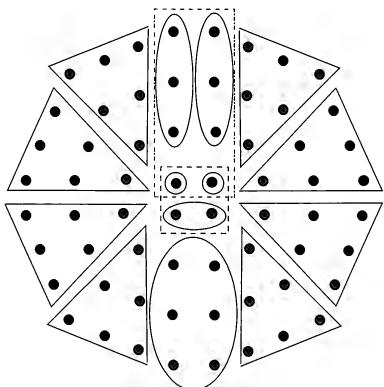
\includegraphics[width=0.62\textwidth]{figs/ch7s5-f64.jpg}
\caption{$\mathbb{F}_{64}$ 中 $x^{64}-x$ 的根按不可约因子聚类的示意 (两个虚线矩形分别框出其中唯一的 $\mathbb{F}_4$ 与 $\mathbb{F}_8$ 拷贝, 它们交于唯一的 $\mathbb{F}_2$ 拷贝).}
\end{figure}

两个虚线矩形框定包含在 $\mathbb{F}_{64}$ 中的 (唯一的) $\mathbb{F}_4$ 与 $\mathbb{F}_8$ 的拷贝; 它们交于 (唯一的) $\mathbb{F}_2$ 的拷贝.

再次, $\mathbb{F}_{64}$ 可以通过用任意一个 $6$ 次不可约多项式生成的理想来商 $\mathbb{F}_2[x]$ 而实现; 这给出了该域的 $9$ 个``不同''的实现.

上面为 $\mathbb{F}_{64}$ 所绘的图几乎毫无意义, 但它可以帮助我们聚焦我们将要提取的关于有限域的最后一点信息. 注意 $\mathbb{F}_{64}$ 的任意自同构的作用必是搅乱图中每个扇区所表示的元素, 而不混合不同扇区的元素, 也不交换扇区. 事实上, 一个扩张的每个自同构都把不可约多项式的根送到同一个多项式的根.

由于有限域的扩张都是单扩张, 我们先前的工作使我们能够精确得多. 把注意力限制在扩张 $\mathbb{F}_p\subseteq\mathbb{F}_{p^d}$ 上, 对素数 $p$, 我们知道这些可以通过一个极小多项式为 $d$ 次的元素实现为单扩张. 这个多项式必可分 ($\mathbb{F}_p$ 是完全的), 所以推论~\ref{cor:autk-count} 立即给出自同构群的大小:
\[
|\Aut_{\mathbb{F}_p}(\mathbb{F}_{p^d})|=d.
\]
但这个群是什么呢?

\begin{proposition}\label{prop:aut-cyclic-frobenius}
$\Aut_{\mathbb{F}_p}(\mathbb{F}_{p^d})$ 是循环群, 由 Frobenius 同构生成.
\end{proposition}

\begin{proof}
设 $\varphi$ 为 Frobenius 同态 $\mathbb{F}_{p^d}\to\mathbb{F}_{p^d}$: $\varphi(x)=x^p$. Frobenius 同态在有限域上是一个同构 (推论~\ref{cor:finite-fields-perfect}) 并且在 $\mathbb{F}_p$ 上限制为恒等 (习题~\ref{ex:frobenius-Fp-identity}), 所以 $\varphi\in\Aut_{\mathbb{F}_p}(\mathbb{F}_{p^d})$. 既然我们事先知道了这个群的大小, 所要证明的只是 $\varphi$ 的阶为 $d$.

设 $e=|\varphi|$. 则 $\varphi^e=\mathrm{id}$; 从而对所有 $x\in\mathbb{F}_{p^d}$ 有 $x^{p^e}=x$. 换言之, (非零) 多项式 $x^{p^e}-x$ 在 $\mathbb{F}_{p^d}$ 中有 $p^d$ 个根; 这推出 $p^d\leq p^e$ (引理~V.\ref{lem:roots-count}). 等价地, $d\leq e$, 得到
\[
|\Aut_{\mathbb{F}_p}(\mathbb{F}_{p^d})|\leq|\varphi|.
\]
但那样这两个数必相等, 因为一个元素的阶总整除群的阶 (习题~II.\ref{ex:lagrange-order}).
\end{proof}

关于有限域还有最后两点评论:
\begin{itemize}
\item[—] 对足够大的 $n$, 惊人地大 (但有限) 的域 $\mathbb{F}_{p^{n!}}$ 可作为代数闭包 $\overline{\mathbb{F}_p}$ 的一个近似: 事实上, 由推论~\ref{cor:factor-xqn}, 这个域包含 $\mathbb{F}_p[x]$ 中所有次数 $\leq n$ 的多项式的根.

这一观察可以转化为 $\overline{\mathbb{F}_p}$ 的一个显式构造: 由推论~\ref{cor:finite-field-extension} 存在扩张
\[
\mathbb{F}_p\subseteq\mathbb{F}_{p^2}\subseteq\mathbb{F}_{p^6}\subseteq\mathbb{F}_{p^{4!}}\subseteq\cdots
\]
并且这个域链的并集给出一个 $\overline{\mathbb{F}_p}$ 的拷贝\footnote{更形式化的构造需要正向极限的概念; 参见 §\hyperref[subsec:limits-colimits]{VIII.1.4}.}.
\item[—] 有限域构成一个范畴, 它 (由推论~\ref{cor:finite-field-extension}) 应强烈地让读者想起在习题~I.\ref{ex:divisibility-category} 中遇到的``玩具''范畴. 然而有一个重要区别: 在那个范畴中每个对象恰有一个自同构, 而我们已经验证有限域可以有许多自同构. 挑战: 读者在一个不同 (但相关) 的语境中遇到过非常相似的情形. 在哪里?
\end{itemize}

\subsection{分圆多项式与分圆域}\label{subsec:cyclotomic}

在前面几节中我们经常遇到 $\mathbb{C}$ 中的 $1$ 的根; 它们生成的扩张非常重要.

设 $n$ 为正整数. 我们将用 $\zeta_n$ 表示复数 $e^{2\pi i/n}$; 于是多项式 $x^n-1$ 在 $\mathbb{C}$ 中的 $n$ 个根就是 $\zeta_n$ 的 $n$ 个不同幂次; 它们构成 $\mathbb{C}$ 的乘法群的一个 $n$ 阶循环子群, 记为 $\mu_n$.\index[sym1]{41@$\mu_n$}\index[sym1]{69@$\zeta_n$}

形象地, $1$ 的根放置在以 $0$ 为中心的正 $n$ 边形的顶点上, 其中一个顶点在 $1$ 处.

\begin{figure}[ht]
\centering
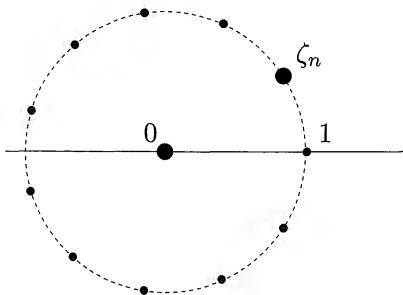
\includegraphics[width=0.4\textwidth]{figs/ch7s5-roots-of-unity.jpg}
\caption{单位根在正 $n$ 边形顶点上的分布.}
\end{figure}

$1$ 的一个 \emph{本原 $n$ 次根} 是 $\mu_n$ 的一个生成元. 于是 $\zeta_n$ 是本原的; 由我们对循环群的工作, 我们知道 (推论~II.\ref{cor:generates}) $\zeta_n^m$ 是一个本原 $n$ 次根当且仅当 $m$ 与 $n$ 互素. 特别地, 有 $\phi(n)$ 个本原的 $1$ 的根, 其中 $\phi$ 是 Euler $\varphi$ 函数 (参见习题~II.\ref{ex:euler-phi-sum}). 从而
\[
\Phi_n(x):=\prod_{\substack{1\leq m\leq n\\ (m,n)=1}}(x-\zeta_n^m)
\]
是一个 $\phi(n)$ 次的多项式.

\begin{definition}\label{def:cyclotomic-poly}
多项式 $\Phi_n(x)$ 称为第 $n$ 个 \emph{分圆多项式}.
\end{definition}

显然 $\Phi_n(x)$ 是一个 $\phi(n)$ 次的首一多项式. 也许不那么显然的是 $\Phi_n(x)$ 有有理 (事实上是整数) 系数, 并且在 $\mathbb{Q}$ 上不可约. 我们马上证明这些事实.

\begin{example}\label{ex:cyclotomic-prime}
若 $n=p$ 为素数, 则 $\mu_p\cong C_p$ 的每个非单位元素都是一个生成元: 除 $1$ 自身外每个 $p$ 次 $1$ 的根都是本原的. 因此
\[
\Phi_p(x)=\frac{x^p-1}{x-1}=x^{p-1}+\cdots+1
\]
就是在例~V.\ref{ex:cyclotomic-eisenstein} 中遇到的特例, 我们在那里证明了 $\Phi_p(x)$ 确实不可约.
\end{example}

如果 $n$ 不是素数呢?

\begin{lemma}\label{lem:cyclotomic-prod}
对所有正整数 $n$,
\[
x^n-1=\prod_{1\leq d\mid n}\Phi_d(x).
\]
\end{lemma}

\begin{proof}
若 $n=de$, 则每个 $d$ 次 $1$ 的根 $\zeta$ 都是 $n$ 次 $1$ 的根, 因为 $\zeta^n=\zeta^{de}=(\zeta^d)^e=1$. 特别地, 每个本原 $d$ 次 $1$ 的根 $\zeta$ 都是 $n$ 次 $1$ 的根.

另一方面, 每个 $\zeta\in\mu_n$ 生成一个子群 $H\subseteq\mu_n$, 且 $H=\mu_d$, 其中 $d$ 等于 $\zeta$ 的阶, 是 $n$ 的一个因子 (命题~II.\ref{prop:subgroups-zn}). 因此每个 $\zeta\in\mu_n$ 对某个 $d\mid n$ 是本原 $d$ 次 $1$ 的根.

由此 $n$ 次 $1$ 的根的集合等于所有 $d\mid n$ 的本原 $d$ 次 $1$ 的根的集合之并. 该陈述立得:
\[
x^n-1=\prod_{\zeta\in\mu_n}(x-\zeta)=\prod_{1\leq d\mid n}\Bigl(\prod_{\zeta\text{ 本原 }d\text{ 次根}}(x-\zeta)\Bigr)=\prod_{1\leq d\mid n}\Phi_d(x),
\]
如所断言.
\end{proof}

这一论证把我们带回到简单的群论考虑. 读者可以验证引理~\ref{lem:cyclotomic-prod} 通过比较所述恒等式两边的其次数立即推出习题~II.\ref{ex:euler-phi-sum} 的结果.

引理~\ref{lem:cyclotomic-prod} 给出了分圆多项式的一个归纳计算; 事实 $\Phi_n(x)\in\mathbb{Z}[x]$ 即由此事实推出. 显式地,

\begin{corollary}\label{cor:cyclotomic-int}
分圆多项式 $\Phi_n(x)$ 有整数系数.
\end{corollary}

\begin{proof}
对 $n$ 用归纳法. 注意 $\Phi_1(x)=x-1$, 并假设我们已经证明了所有 $m<n$ 的 $\Phi_m(x)$ 都有整数系数. 特别地,
\[
f(x):=\prod_{\substack{1\leq d\mid n\\ d<n}}\Phi_d(x)
\]
是一个有整数系数的首一多项式. 由于 $f(x)$ 首一, 我们可以在 $\mathbb{Z}[x]$ 中用它去除 $x^n-1$ 带余: $\exists\,q(x),r(x)\in\mathbb{Z}[x]$ 使得
\[
x^n-1=f(x)q(x)+r(x),
\]
其中 $r(x)=0$ 或 $\deg r(x)<\deg f(x)$. 另一方面, 由引理~\ref{lem:cyclotomic-prod},
\[
x^n-1=f(x)\Phi_n(x)
\]
在 $\mathbb{C}[x]$ 中. 因此在 $\mathbb{C}[x]$ 中
\[
f(x)\bigl(\Phi_n(x)-q(x)\bigr)=r(x).
\]
但这迫使 $r(x)=0$ (否则我们会有 $\deg r(x)\geq\deg f(x)$). 因此 $\Phi_n(x)=q(x)\in\mathbb{Z}[x]$.
\end{proof}

\begin{example}\label{ex:cyclotomic-examples}
读者可以花些高质量的时间显式计算几个非素数 $n$ 的分圆多项式 $\Phi_n(x)$, 用归纳法并利用我们已经知道素数的显式 $\Phi_p(x)$.

例如, $x^4-1=\Phi_1(x)\Phi_2(x)\Phi_4(x)$; 因此
\[
\Phi_4(x)=\frac{x^4-1}{x^2-1}=x^2+1.
\]
由于 $x^6-1=\Phi_1(x)\Phi_2(x)\Phi_3(x)\Phi_6(x)$,
\[
\Phi_6(x)=\frac{x^6-1}{(x^2-1)(x^2+x+1)}=x^2-x+1.
\]
由于 $x^{12}-1=\Phi_1(x)\Phi_2(x)\Phi_3(x)\Phi_4(x)\Phi_6(x)\Phi_{12}(x)$,
\[
\Phi_{12}(x)=\frac{x^{12}-1}{(x^6-1)(x^2+1)}=x^4-x^2+1,
\]
如此等等, 不一而足.

乐观的读者现在可能开始猜测 $\Phi_n(x)$ 的系数总是 $0$ 或 $\pm 1$ (如果我们不知道真相, 我们也会这样猜). 显然第一个反例出现在 $n=105$ (习题~\ref{ex:cyclotomic-1-15}); 并且已知当 $n\gg 0$ 时系数可以任意大.
\end{example}

$\Phi_n(x)$ 的不可约性稍微棘手一些, 特别是因为可分性溜进了标准论证 (这正是我们不得不等到现在才陈述它的原因).

\begin{proposition}\label{prop:cyclotomic-irred}
对所有正整数 $n$, $\Phi_n(x)\in\mathbb{Z}[x]$ 在 $\mathbb{Q}$ 上不可约.

(由于 $\Phi_n(x)$ 首一, 在 $\mathbb{Q}[x]$ 中的不可约性等价于在 $\mathbb{Z}[x]$ 中的不可约性; 参见推论~V.\ref{cor:irreducible-poly-equiv}.)
\end{proposition}

\begin{proof}
反证法, 假设 $\Phi_n(x)$ 可约. 则它的根 $\zeta_n^m$, 其中 $(m,n)=1$, 分布到各个因子中; 我们可以选取一个不可约首一因子 $f(x)$ 的一个根 $\zeta_n^m$, 使得另一个根 $\zeta_n^{mp}$ (对某个不整除 $n$ 的素数 $p$) 不是 $f(x)$ 的根. 写
\[
\Phi_n(x)=f(x)g(x);
\]
由于 $\Phi_n(x)\in\mathbb{Z}[x]$ 且 $\Phi_n(x)$, $f(x)$ 首一, 则 $f(x)$ 与 $g(x)$ 有整数系数 (参见习题~V.\ref{ex:poly-split-rx}). 由我们的选择, $f(x)$ 是 $\zeta_n^m$ 在 $\mathbb{Q}$ 上的极小多项式, 且 $g(\zeta_n^{mp})=0$.

由此 $\zeta_n^m$ 是 $g(x^p)$ 的一个根, 从而 $f(x)\mid g(x^p)$. 因此我们可以写
\[
g(x^p)=f(x)h(x)
\]
其中 $h(x)\in\mathbb{Z}[x]$. 把最后一个等式模 $p$ 读出来, 我们得到 (再次利用习题~\ref{ex:frobenius-Fp-identity}, 并用下划线表示陪集)
\[
\underline{g}(x)^p=\underline{f}(x)\underline{h}(x)\quad\text{在 }\mathbb{F}_p[x]\text{ 中};
\]
特别地, $\underline{f}(x)$ 与 $\underline{g}(x)$ 在 $\mathbb{F}_p[x]$ 中必有一个非平凡公因子 $\underline{\ell}(x)$. 但那样
\[
\underline{\ell}(x)^2\mid\underline{f}(x)\underline{g}(x):
\]
$\Phi_n(x)$ 模 $p$ 的归约必有一个重因子.

这推出 $x^n-1\in\mathbb{F}_p[x]$ 有一个重因子; 即它不可分. 然而它的导数 $nx^{n-1}\in\mathbb{F}_p[x]$ 非零 (因为由假设 $p$ 不整除 $n$), 而引理~\ref{lem:separable-gcd} 推出 $x^n-1$ 在 $\mathbb{F}_p[x]$ 中可分.

这一矛盾表明我们假设 $\Phi_n(x)$ 可约是荒谬的, 证明了该陈述. \qed
\end{proof}

\begin{definition}\label{def:cyclotomic-field}
多项式 $x^n-1$ 在 $\mathbb{Q}$ 上的分裂域 $\mathbb{Q}(\zeta_n)$ 是第 $n$ 个 \emph{分圆域}.
\end{definition}

由命题~\ref{prop:cyclotomic-irred}, $\mathbb{Q}(\zeta_n)$ 是 $\mathbb{Q}$ 的一个 $\phi(n)$ 次扩张; $\Phi_n(x)$ 是 $\zeta_n$ 的极小多项式.

像往常一样, 我们现在关注这个扩张的自同构群, 并且像在先前的例子中一样情形非常清晰.

\begin{proposition}\label{prop:aut-cyclotomic}
$\Aut_{\mathbb{Q}}(\mathbb{Q}(\zeta_n))$ 同构于 $\mathbb{Z}/n\mathbb{Z}$ 中的单位群.
\end{proposition}

\begin{proof}
我们知道 $\Aut_{\mathbb{Q}}(\mathbb{Q}(\zeta_n))$ 的基数为 $\phi(n)$ (推论~\ref{cor:autk-count}; 根互异因为 $\Phi_n(x)$ 可分), 所以我们只要给出一个单同态
\[
j:(\mathbb{Z}/n\mathbb{Z})^*\to\Aut_{\mathbb{Q}}(\mathbb{Q}(\zeta_n)).
\]
对 $[m]_n\in(\mathbb{Z}/n\mathbb{Z})^*$, 即对一个与 $n$ 互素的整数 $m$, 令 $j([m]_n)$ 为唯一的把 $\zeta_n$ 送到 $\zeta_n^m$ 的 $\mathbb{Q}(\zeta_n)\to\mathbb{Q}(\zeta_n)$ 的自同构 (参见命题~\ref{prop:simple-ext-iso-lift});
这显然与代表元 $m$ 的选择无关. 则 $j$ 显然单, 且
\[
j([m_1]_n)\circ j([m_2]_n)(\zeta_n)=j([m_1]_n)(\zeta_n^{m_2})=\zeta_n^{m_2m_1}
\]
与 $j([m_1m_2]_n)$ 的作用一致, 表明 $j$ 是一个同态, 完成证明. \qed
\end{proof}

\begin{example}\label{ex:splitting-x8-1-aut}
读者应当重新考虑例~\ref{ex:x8-1-splitting}: 由我们刚刚证明的, $x^8-1$ 的分裂域的自同构群同构于 $\mathbb{Z}/8\mathbb{Z}$ 中的单位群; 这个群立刻可见同构于 $(\mathbb{Z}/2\mathbb{Z})\times(\mathbb{Z}/2\mathbb{Z})$, 确认了例~\ref{ex:x8-1-splitting} 中作出的断言.
\end{example}

正 $n$ 边形用直尺与圆规的可构造性当然等价于复数 $\zeta_n$ 的可构造性. 既然我们现在知道 $[\mathbb{Q}(\zeta_n):\mathbb{Q}]=\phi(n)$, 推论~\ref{cor:constructible-degree} 告诉我们正 $n$ 边形能用直尺与圆规构造仅当 $\phi(n)$ 是 $2$ 的幂. 这个条件可以追得更远 (习题~\ref{ex:regular-n-gon-constructible}). 无论如何, 在我们吸收了一点 Galois 理论之后, 我们将再次回到这个主题.

\subsection{可分性与单扩张}\label{subsec:separability-simple}

我们迄今遇到的所有域扩张的例子都是单扩张, 尽管有时这起初并不完全明显 (参见例~\ref{ex:sqrt2-sqrt3}). 这有一个很好的理由: 我们看到的大多数例子都是可分扩张, 而我们现在可以证明一个有限可分扩张必是单的.

这里是一个单扩张的漂亮判据 (它不涉及任何可分性条件):

\begin{proposition}\label{prop:simple-inter-finite}
一个代数扩张 $k\subseteq F$ 是单的当且仅当不同的中间域 $k\subseteq E\subseteq F$ 的数目有限.
\end{proposition}

\begin{proof}
假设 $F=k(\alpha)$ 是单且代数的, 并设 $q_k(x)$ 为 $\alpha$ 在 $k$ 上的极小多项式. 把 $F$ 嵌入 $k$ 的一个代数闭包 $\overline{k}$ 中. 若 $E$ 是一个中间域, 则 $F=E(\alpha)$ 也是一个单的、代数的扩张; 记 $q_E(x)$ 为 $\alpha$ 在 $E$ 上的极小多项式. 由于对所有 $E$ 有 $q_k(x)\in E[x]$ 且 $q_k(\alpha)=0$, 我们知道每个 $q_E(x)$ 是 $q_k(x)$ 的一个因子.

我们断言 $E$ 其实由 $q_E(x)$ 决定. 由于 $q_k(x)$ 在 $\overline{k}$ 中只有有限多个因子, 这就证明了只有有限多个中间域, 即陈述的``仅当''部分.

为验证我们的断言, 我们将证明 $E$ 由 $q_E(x)$ 的系数 (在 $k$ 上) 生成. 为看清这一点, 令 $E'$ 为 $E$ 中由 $k$ 与 $q_E(x)$ 的系数生成的子域. 则 $q_E(x)\in E'[x]$, 并且由于 $q_E(x)$ 在 $E$ 上不可约, 它在 $E'$ 上必不可约. 注意 $E'(\alpha)=F=E(\alpha)$. 我们有 $E'\subseteq E\subseteq F$; 因此
\[
\deg(q_E(x))=[F:E']=[F:E][E:E']=\deg(q_E(x))[E:E'],
\]
由此 $[E:E']=1$; 即 $E=E'$, 如所需. 这就完成了陈述的``仅当''部分的证明.

为证明``当''部分, 假设只有有限多个中间域 $k\subseteq E\subseteq F$. 扩张 $k\subseteq F$ 必是有限生成的 (否则我们可以构造一个无限子扩张链 $k\subseteq k(\alpha_1)\subseteq k(\alpha_1,\alpha_2)\subseteq\cdots\subseteq F$, 从而会有无限多个中间域), 因此由于它是代数的而是有限的. 若 $k$ 是有限域, 则 $F$ 也是, 并且该扩张由推论~\ref{cor:finite-field-extension} 自动是单的; 因此我们可以假设 $k$ 是无限的, 并且我们要证明每个有限生成的代数扩张 $F=k(\alpha_1,\ldots,\alpha_r)$ 是单的.

用归纳法, 我们不妨设 $F=k(\alpha,\beta)$. 对每个 $c\in k$, 我们有中间域
\[
k(c\alpha+\beta)\subseteq k(\alpha,\beta).
\]
但只有有限多个中间域, 而 $k$ 是无限的, 所以对某些 $c\neq c'\in k$ 必有
\[
k(c'\alpha+\beta)=k(c\alpha+\beta).
\]
由此
\[
\alpha=\frac{(c'\alpha+\beta)-(c\alpha+\beta)}{c'-c}\in k(c\alpha+\beta)\quad\text{且}\quad\beta=(c\alpha+\beta)-c\alpha\in k(c\alpha+\beta)
\]
因此 $k(\alpha,\beta)\subseteq k(c\alpha+\beta)$. 另一包含平凡成立, 所以 $k(\alpha,\beta)=k(c\alpha+\beta)$ 是单的.
\end{proof}

这里是与可分性的联系:

\begin{proposition}\label{prop:finite-sep-simple}
每个有限可分扩张都是单的.
\end{proposition}

\begin{proof}
像命题~\ref{prop:simple-inter-finite} 的证明中那样用归纳法, 我们不妨设 $F=k(\alpha,\beta)$, 其中 $\alpha$ 与 $\beta$ 在 $k$ 上可分 (从而特别地是代数的), 并且我们可以假设 $k$ 是无限域.

考虑嵌入 $\iota:F\hookrightarrow\overline{k}$ 的集合 $I$, 即 $F$ 到 $k$ 的代数闭包中、扩张 $k$ 的恒等的嵌入. 若 $\iota\neq\iota'\in I$ 且 $x$ 是一个不定元, 则多项式
\[
\iota(\alpha)x+\iota(\beta),\qquad\iota'(\alpha)x+\iota'(\beta)
\]
是不同的: 否则 $\iota'(\alpha)=\iota(\alpha)$ 且 $\iota'(\beta)=\iota(\beta)$, 从而 $\iota,\iota'$ 会在整个 $k(\alpha,\beta)$ 上以相同方式作用, 迫使 $\iota=\iota'$.

\index{duoxiangshi@多项式(polynomial)!shouyi@首一(monic)}因此多项式
\[
f(x)=\prod_{\iota\neq\iota'}\bigl((\iota(\alpha)x+\iota(\beta))-(\iota'(\alpha)x+\iota'(\beta))\bigr)\in\overline{k}[x]
\]
不恒为 $0$. 由于 $k$ 无限, 由此 $\exists\,c\in k$ 使得 $f(c)\neq 0$; 即不同的 $\iota\in I$ 把
\[
\gamma=c\alpha+\beta
\]
送到不同的元素
\[
\iota(\gamma)=\iota(\alpha)c+\iota(\beta)
\]
(每个 $\iota$ 扩张 $\mathrm{id}_k$, 所以 $\iota(c)=c$). 由于 $I$ 的基数为 $[F:k]_s$ (定义~\ref{def:separable-degree}) 且每个 $\iota(\gamma)$ 是 $\gamma$ 在 $k$ 上的极小多项式的一个根, 我们有
\[
[F:k]_s\leq[k(\gamma):k]\leq[F:k].
\]
由假设该扩张可分, 所以由命题~\ref{prop:finite-sep-degree} 知 $[F:k]_s=[F:k]$, 推出 $[k(\gamma):k]=[F:k]$ 并最后
\[
F=k(\gamma),
\]
完成证明.
\end{proof}

命题~\ref{prop:finite-sep-simple} 很好地说明了为什么可分性是一个技术上令人满意的条件. 为了更进一步强调这一点, 注意我们现在可以把推论~\ref{cor:autk-count} 中找到的方便的不等式推广到所有有限可分扩张:

\begin{corollary}\label{cor:aut-ineq}
设 $k\subseteq F$ 为一个有限、可分扩张. 则
\[
|\Aut_k(F)|\leq[F:k],
\]
等号成立当且仅当 $k\subseteq F$ 是正规扩张.
\end{corollary}

\begin{proof}
由于 $k\subseteq F$ 有限且可分, 命题~\ref{prop:finite-sep-simple} 推出它是单的: 对某个 $\alpha\in F$ 有 $F=k(\alpha)$. 该不等式由推论~\ref{cor:autk-count} 立得, 且等号成立当且仅当 $\alpha$ 的极小多项式 $f(x)$ 在 $F$ 中分解为互异的一次因子. 在此情形下 $F$ 是 $f(x)$ 的分裂域, 所以由定理~\ref{thm:finite-normal-splitting} 它在 $k$ 上正规. 反过来, 若 $F$ 在 $k$ 上正规, 则 $f(x)$ 在 $F$ 中完全分裂并且由于 $\alpha$ 在 $k$ 上可分而有互异的根; 因此 $|\Aut_k(F)|=[F:k]$, 再次由推论~\ref{cor:autk-count}. \qed
\end{proof}

\begin{example}\label{ex:non-simple-insep}
由命题~\ref{prop:finite-sep-simple}, 如果我们想构造一个非单的有限扩张, 我们必须使用不可分元素; 为给出一个例子, 我们把例~\ref{ex:xp-t-insep} 稍微加工一下. 考虑两个变量上的有理函数域 $F=\mathbb{F}_p(u,v)$ 与子域 $k=\mathbb{F}_p(s,t)$, 其中 $s=u^p$ 且 $t=v^p$. 则 $k\subseteq F$ 是一个代数扩张; $u$ 在 $k$ 上的极小多项式是 $x^p-s$; $v$ 在 $k(u)$ 上的极小多项式是 $y^p-t$; 由此
\[
[F:k]=p^2.
\]
当 $c$ 取遍 $k$ 时, 我们得到中间域
\[
k\subseteq k(cu+v)\subseteq F.
\]
若任意两个选择 $c$, $c'$ 导致相同的中间域, 则我们会像命题~\ref{prop:simple-inter-finite} 的证明中那样推出 $k(u,v)=k(cu+v)$. 特别地, 我们会有
\[
[k(cu+v):k]=p^2.
\]
但事实并非如此, 因为 $(cu+v)^p=c^ps+t\in k(s,t)=k$; 从而 $cu+v$ 在 $k$ 上的极小多项式的次数至多为 $p$. 由于 $k=\mathbb{F}_p(s,t)$ 无限, 有无限多个中间域, 并由此 (由命题~\ref{prop:simple-inter-finite}) 推出 $F$ 不是 $k$ 的一个单扩张.
\end{example}

\subsection*{习题}
\phantomsection
\addcontentsline{toc}{subsection}{习题}

\begin{prob}\label{ex:finite-field-additive}
设 $p>0$ 为素数. 证明阶为 $p^d$ 的有限域的加法群同构于 $(\mathbb{Z}/p\mathbb{Z})^d$.
\end{prob}

\begin{prob}\label{ex:sum-of-two-squares}
证明有限域 $F$ 的每个元素都是 $F$ 中两个平方之和. (提示: 记住 $F$ 的乘法群是循环的.)
\end{prob}

\begin{prob}\label{ex:finite-field-iso-F8}
$\triangleright$ 找出一个显式同构
\[
\frac{\mathbb{F}_2[x]}{(x^3+x^2+1)}\xrightarrow{\sim}\frac{\mathbb{F}_2[x]}{(x^3+x+1)}.
\]
[§\ref{subsec:finite-fields}]
\end{prob}

\begin{prob}\label{ex:irred-deg4-F2}
$\triangleright$ 找出 $\mathbb{F}_2$ 上所有 $4$ 次不可约多项式, 并数出 $5$ 次的个数. [§\ref{subsec:finite-fields}]
\end{prob}

\begin{prob}\label{ex:irred-deg12-F9}
找出 $\mathbb{F}_9$ 上 $12$ 次不可约多项式的数目.
\end{prob}

\begin{prob}\label{ex:F16-frobenius-action}
用 $\mathbb{F}_{16}$ 作为 $\mathbb{F}_2[x]$ 的商的任一实现, 显式写出循环群 $C_4$ 在 $\mathbb{F}_{16}$ 上的作用 (即作为 $\mathbb{F}_2$-向量空间的线性变换).
\end{prob}

\begin{prob}\label{ex:frobenius-rational-canonical}
设 $p$ 为素数. 把 Frobenius 自同构 $\varphi:\mathbb{F}_{p^d}\to\mathbb{F}_{p^d}$ 视为 $\mathbb{F}_{p^d}$ 的 $\mathbb{F}_p$-向量空间上的线性变换. 找出 $\varphi$ 的有理标准形. (改造命题~\ref{prop:aut-cyclic-frobenius} 的证明以说明 $\varphi$ 的极小多项式是 $x^d-1$.)
\end{prob}

\begin{prob}\label{ex:factor-Phi-p-Fp}
对素数 $p$, 找出 $\Phi_p(x)$ 在 $\mathbb{F}_p$ 上的分解.
\end{prob}

\begin{prob}\label{ex:cyclotomic-1-15}
$\triangleright$ 找出所有 $1\leq n\leq 15$ 的分圆多项式 $\Phi_n(x)$. 计算 $\Phi_{105}(x)$. [§\ref{subsec:cyclotomic}]
\end{prob}

\begin{prob}\label{ex:cyclotomic-2m}
找出所有 $m\geq 0$ 的 $\Phi_{2^m}(x)$.
\end{prob}

\begin{prob}\label{ex:Phi-2n-Phi-n}
证明若 $n>1$ 为奇数, 则 $\Phi_{2n}(x)=\Phi_n(-x)$. (提示: 把本原 $14$ 次 $1$ 的根与本原 $7$ 次 $1$ 的根并列画出; 然后回到习题~II.\ref{ex:euler-phi-odd} 以证明你所观察到的现象.)
\end{prob}

\begin{prob}\label{ex:Phi-n-divides}
$\neg$ 设 $a,n$ 为正整数, 且 $a>1$. 证明若 $\Phi_n(a)$ 整除 $a-1$, 则 $n=1$. (记住 $\Phi_n(a)$ 是复数 $a-\zeta$ 的乘积, 其中 $\zeta$ 是本原 $n$ 次 $1$ 的根. 这告诉你关于 $\Phi_n(a)$ 的大小的什么信息?) [命题~\ref{prop:cyclotomic-irred}]
\end{prob}

\begin{prob}\label{ex:Phi-n-quotient}
$\neg$ 设 $a,d,n$ 为正整数, 且 $d<n$, $a>1$. 假设 $a^d-1$ 整除 $a^n-1$. 证明 $\Phi_n(a)$ 整除商 $(a^n-1)/(a^d-1)$. (提示: 习题~V.\ref{ex:ca-1-divides}.) [命题~\ref{prop:cyclotomic-irred}]
\end{prob}

\index{Witt@Witt!Ernst@Ernst}\begin{prob}\label{ex:wedderburn-witt}
$\triangleright$ 设 $R$ 为一个有限除环.
\begin{itemize}
\item 证明 $R$ 的中心 (习题~III.\ref{ex:center}) 同构于 $\mathbb{F}_q$, 其中 $q$ 为素数幂. 证明 $|R|=q^n$ 对某个 $n$.
\item 对每个 $r\in R$, 证明 $(R^*,\cdot)$ 的乘法群中 $r$ 的中心化子的阶为 $q^d-1$ 对某个 $d\leq n$.
\item 证明存在整数 $d_1,\ldots,d_r<n$ 使得
\begin{equation}
q^n-1=q-1+\sum_{i=1}^r\frac{q^n-1}{q^{d_i}-1}.
\tag{*}\end{equation}
(提示: 类方程.)
\item 推出 $\Phi_n(q)$ 整除 $q-1$, 从而 $n=1$. (利用习题~\ref{ex:Phi-n-divides} 与 \ref{ex:Phi-n-quotient}.)
\item 推出 $R$ 等于其中心, 表明 $R$ 是交换的.
\end{itemize}
\index{Wedderburn@Wedderburn!Joseph@Joseph!xiaodingli@小定理(little theorem)!xiemi@楔幂(wedge power)}于是每个有限除环都是一个域: 这就是 Wedderburn 的小定理. 这里给出的论证属于 Ernst Witt. [§III.\ref{subsec:ring-examples}]
\end{prob}

\begin{prob}\label{ex:Phi-n-mod-p}
$\triangleright$ 设 $a,p,n$ 为整数, 其中 $p,n$ 为正且 $p$ 为素数, $p\nmid n$.
\begin{itemize}
\item 证明 $x^n-1$ 模 $p$ 无重根.
\item 证明若 $p$ 整除 $\Phi_n(a)$, 则 $a^n\equiv 1\pmod p$. (特别地, $p\nmid a$, 故 $[a]_p\in(\mathbb{Z}/p\mathbb{Z})^*$.)
\item 证明若 $p$ 整除 $\Phi_n(a)$, 则对一切 $d<n$ 有 $a^d\not\equiv 1\pmod p$.
\item 推出 $p\mid\Phi_n(a)$ 当且仅当 $[a]_p$ 在 $(\mathbb{Z}/p\mathbb{Z})^*$ 中的阶为 $n$.
\item 计算 $\Phi_{15}(9)$, 并证明它被 $31$ 整除. 然后回看习题~II.\ref{ex:order-9-31} 的第一部分.
\end{itemize}
[§II.\ref{subsec:iso-groups}, 习题~\ref{ex:primitive-prime-divisor}, 习题~\ref{ex:p-congruence-1-mod-n}]
\end{prob}

\begin{prob}\label{ex:primitive-prime-divisor}
\index{Birkhoff–Vandiver dingli@Birkhoff–Vandiver 定理(Birkhoff-Vandiver theorem)}若 $q$ 是一个整除 $a^n-1$ 且对任意 $d<n$ 不整除 $a^d-1$ 的素数, 则称 $q$ 为 $a^n-1$ 的一个 \emph{本原素因子}. 由习题~\ref{ex:Phi-n-mod-p}, 若 $q\nmid n$ 且 $q\mid\Phi_n(a)$, 则 $q$ 是 $a^n-1$ 的一个本原素因子. Birkhoff--Vandiver 定理断言 $a^n-1$ 对所有但极少数例外都有本原素因子: $n=1$, $a=2$; $n=2$, $a+1$ 是 $2$ 的幂; 以及 $n=6$, $a=2$.

\index{Lichiardopol@Lichiardopol!Nicolas@Nicolas}假设这一陈述, 我们可以给出 Wedderburn 定理的另一个证明 (由 Nicolas Lichiardopol 于 $2003$ 年发表). 设 $R$ 为一个有限除环.
\begin{itemize}
\item 证明存在素数 $p$ 使得 $|R|=p^n$ 对某个整数 $n$.
\item 若 $n=1$, 则 $R\cong\mathbb{F}_p$. 若 $n=2$ 或 $p=2$ 且 $n=6$, 则 $R$ 是交换的: 读者已在习题~III.\ref{ex:division-p2} 与 IV.\ref{ex:wedderburn-64} 中证明了这一点.
\item 因此, 由 Birkhoff--Vandiver 我们不妨假设 $p^n-1$ 有一个本原素因子 $p'$.
\item 证明在 $R$ 的乘法群 $(R^*,\cdot)$ 中存在一个阶为 $p'$ 的元素 $a$.
\item 证明 $R$ 是包含 $a$ 的 $R$ 的唯一子除环.
\item 证明 $a$ 在 $R$ 中的中心化子 (习题~III.\ref{ex:centralizer}) 就是 $R$ 自身; 推出 $a$ 在 $R$ 的中心中 (习题~III.\ref{ex:center}).
\item 证明 $R$ 的中心就是 $R$: 这表明 $R$ 是交换的.
\end{itemize}
于是 $R$ 是一个有限域.

注意 Birkhoff--Vandiver 定理给出了另一个快速方式来完成 Witt 的证明: $q^n-1$ 的一个本原素因子会由 $(*)$ 整除 $q-1$, 表明 $n=1$.
\end{prob}

\begin{prob}\label{ex:p-congruence-1-mod-n}
$\neg$ 设 $a,p,n$ 为整数, 其中 $p,n$ 为正且 $p$ 为素数, $p\nmid n$. 假设 $p$ 整除 $\Phi_n(a)$. 证明 $p\equiv 1\bmod n$. (利用习题~\ref{ex:Phi-n-mod-p}.) [习题~\ref{ex:inf-many-primes-1-mod-n}]
\end{prob}

\begin{prob}\label{ex:inf-many-primes-1-mod-n}
$\triangleright$ 设 $n>0$ 为任意整数. 证明存在无穷多个素数整数 $\equiv 1\bmod n$. (利用习题~\ref{ex:p-congruence-1-mod-n} 与习题~V.\ref{ex:euclid-variation-primes}.)

\index{Dirichlet@Dirichlet!Peter Gustav Lejeune@Peter Gustav Lejeune}这一练习的结果就是 Dirichlet 关于算术级数中的素数的定理的一个特例; 参见 §\ref{subsec:abelian-galois-q}. [\S\ref{subsec:abelian-galois-q}]
\end{prob}

\begin{prob}\label{ex:regular-n-gon-constructible}
$\triangleright$ 证明正 $n$ 边形能用直尺与圆规构造仅当 $n=2^m p_1\cdots p_r$, 其中 $m\geq 0$ 且因子 $p_i$ 是互异的 Fermat 素数. (提示: 利用习题~V.\ref{ex:zn-crt-phi} 与推论~\ref{cor:constructible-degree}.) [§\ref{subsec:cyclotomic}, §\ref{subsec:constructible-ngons}]
\end{prob}

\begin{prob}\label{ex:matrix-contains-extension-finite}
回忆由习题~\ref{ex:matrix-contains-extension}, $k$ 上次数 $\leq n$ 的每个域扩张都是矩阵环 $\mathcal{M}_n(k)$ 的一个子 $k$-代数. 证明若 $k$ 有限或特征为 $0$, 则包含在 $\mathcal{M}_n(k)$ 中的每个 $k$ 的扩张都有次数 $\leq n$.
\end{prob}

\begin{prob}\label{ex:splitting-of-separable}
证明若 $k\subseteq F$ 是一个可分多项式的分裂域, 则它也是一个不可约可分多项式的分裂域.
\end{prob}

\begin{prob}\label{ex:separable-generation}
$\neg$ 设 $k$ 为无限域. 若 $F=k(\alpha_1,\ldots,\alpha_r)$, 其中每个 $\alpha_i$ 在 $k$ 上可分, 证明存在 $c_1,\ldots,c_r\in k$ 使得 $F=k(c_1\alpha_1+\cdots+c_r\alpha_r)$.
\end{prob}

\begin{prob}\label{ex:no-irred-no-sep-extension}
$\triangleright$ 设 $k$ 为一个域, 并设 $n>0$ 为整数. 假设在 $k[x]$ 中不存在 $n$ 次不可约多项式. 证明不存在 $k$ 的 $n$ 次可分扩张. [§\ref{subsec:ft-algebra}]
\end{prob}

\section{一点 Galois 理论}\label{sec:galois-theory}

Galois 理论是域论与群论之间优美的交互, 其动机最初来自确定多项式根之间``对称性''的问题. Galois 关心的是多项式的根之间必然成立的具体关系, 其中最平凡的例子莫过于: 若 $\alpha,\beta$ 是 $x^2+px+q$ 的根, 则 $\alpha+\beta=-p$ 且 $\alpha\beta=q$. 交换根 $\alpha,\beta$ 对量 $\alpha+\beta,\alpha\beta$ 毫无影响. 更一般地, 对高次多项式, 可能存在若干在根的某些置换下保持不变的量. 这些量以及相应的置换群可以看作由该多项式决定的不变量, 从而给出一个研究该多项式的精妙工具.

\subsection{Galois 对应与 Galois 扩张}\label{subsec:galois-correspondence}

在域论的语言中, 多项式 $f(x)$ 的根的子集决定了 $f(x)$ 分裂域的中间域, 而根的置换群给出这些中间域的自同构. 有见于此, 分裂域走到台前毫不意外; 我们能够用自同构群刻画此类域 (下述定理~\ref{thm:galois-equivalence}) 这一事实, 将是整个讨论的关键.

在涉入这些水域之前, 我们应当把扩张的自同构群与中间域之间的精确关系形式化.

\begin{definition}\label{def:fixed-field}
\index{budongyu@不动域(fixed field)}设 $k\subseteq F$ 为域扩张, 并设 $G\subseteq\Aut_k(F)$ 是此扩张的一个自同构群. $G$ 的\emph{不动域}是中间域\index[sym1]{04@$\Aut_k(F)$}
\[
F^G:=\{\alpha\in F\mid \forall g\in G,\; g\alpha=\alpha\}.
\]
$F^G$ 确实是包含 $k$ 的 $F$ 的子域, 这一点是显然的. 不动域的概念使我们可以建立一个对应
\[
\begin{tikzcd}[column sep=3em]
\{\text{中间域 }E:k\subseteq E\subseteq F\} \ar[r,shift left=.7ex] & \{\Aut_k(F)\text{ 的子群}\} \ar[l,shift left=.7ex]
\end{tikzcd},
\]
它把中间域 $E$ 映到 $\Aut_k(F)$ 的子群 $\Aut_E(F)$, 把子群 $G\subseteq\Aut_k(F)$ 映到不动域 $F^G$.
\end{definition}

\begin{definition}\label{def:galois-correspondence}
这被称为 \emph{Galois 对应}.
\end{definition}

\begin{lemma}\label{lem:galois-correspondence-inclusion}
Galois 对应是反包含的. 进一步, 对 $\Aut_k(F)$ 的所有子群 $G$ 与所有中间域 $k\subseteq E\subseteq F$:
\begin{itemize}
\item $E\subseteq F^{\Aut_E(F)}$;
\item $G\subseteq\Aut_{F^G}(F)$.
\end{itemize}
此外, 记 $E_1E_2$ 为包含中间域 $E_1,E_2$ 的 $F$ 的最小子域, 记 $\langle G_1,G_2\rangle$ 为包含子群 $G_1,G_2$ 的 $\Aut_k(F)$ 的最小子群. 则
\begin{itemize}
\item $\Aut_{E_1E_2}(F)=\Aut_{E_1}(F)\cap\Aut_{E_2}(F)$;
\item $F^{\langle G_1,G_2\rangle}=F^{G_1}\cap F^{G_2}$.
\end{itemize}
\end{lemma}

\begin{proof}
习题~\ref{ex:galois-ft-lemma}.
\end{proof}

当然, 读者应当开始猜想: 是否存在某些情形能保证引理~\ref{lem:galois-correspondence-inclusion} 中的包含关系成为等式, 从而使 Galois 对应成为双射. 这正是我们前进的方向. 第一个观察是这并非总成立:

\begin{example}\label{ex:cube-root-2-not-galois}
考虑扩张 $\mathbb{Q}\subseteq\mathbb{Q}(\sqrt[3]{2})$. 由于
\[
[\mathbb{Q}(\sqrt[3]{2}):\mathbb{Q}]=3
\]
是素数, 唯一的中间域是 $\mathbb{Q}$ 与 $\mathbb{Q}(\sqrt[3]{2})$ (由推论~\ref{cor:degree-divides}). 关于 $\Aut_{\mathbb{Q}}(\mathbb{Q}(\sqrt[3]{2}))$, 由于 $\sqrt[3]{2}\in\mathbb{R}$, 我们有一个扩张 $\mathbb{Q}(\sqrt[3]{2})\subseteq\mathbb{R}$; 又由于 $\sqrt[3]{2}$ 是 $\mathbb{R}$ 中 $2$ 的唯一立方根, 我们看到 $\sqrt[3]{2}$ 的极小多项式 $t^3-2$ 在 $\mathbb{Q}(\sqrt[3]{2})$ 中只有一个根. 由推论~\ref{cor:autk-count}, $\Aut_{\mathbb{Q}}(\mathbb{Q}(\sqrt[3]{2}))$ 由单个元素组成: 它是平凡的.

\index{dandianji@单点集(singleton)}于是, 在此例中 Galois 对应在两个元素组成的集合与单点集之间作用:
\[
\begin{tikzcd}[column sep=3em]
\{\mathbb{Q},\mathbb{Q}(\sqrt[3]{2})\} \ar[r,shift left=.7ex] & \{\Aut_{\mathbb{Q}}(\mathbb{Q}(\sqrt[3]{2}))\}=\{e\} \ar[l,shift left=.7ex]
\end{tikzcd}.
\]
特别地, 把每个中间域映到相应自同构群的函数一般不是单射.

这个例子表明引理~\ref{lem:galois-correspondence-inclusion} 中的包含 $E\subseteq F^{\Aut_E(F)}$ 可能是真包含: $\mathbb{Q}$ 真包含于 $\mathbb{Q}(\sqrt[3]{2})$, 而后者是自同构群 (唯一) 子群的不动域. 所幸, 另一个包含关系受到更多限制:
\end{example}

\begin{proposition}\label{prop:aut-fixed-field-degree}
设 $k\subseteq F$ 为有限扩张, 并设 $G$ 是 $\Aut_k(F)$ 的一个子群. 则 $|G|=[F:F^G]$, 且
\[
G=\Aut_{F^G}(F).
\]
特别地, 对有限扩张, Galois 对应 (从中间域到自同构群) 是满射.
\end{proposition}

证明这一事实引导我们仔细考察形如 $F^G\subseteq F$ 的有限扩张. 出人意料的是, 它们恰好满足我们迄今遇到的几乎所有性质:

\begin{lemma}\label{lem:fixed-field-ext-props}
设 $k\subseteq F$ 为有限扩张, 并设 $G$ 是 $\Aut_k(F)$ 的一个子群. 则 $F^G\subseteq F$ 是有限, 单, 正规, 可分的扩张.
\end{lemma}

\begin{remark}\label{rmk:galois-orbit-poly}
本引理的关键在于如下值得强调的观察.

若 $\alpha\in F$ 且 $g\in G$, 注意 $g\alpha$ 必是 $\alpha$ 在 $k$ 上的极小多项式的根; 根只有有限多个, 所以 $G$ 在 $\alpha$ 上的轨道由有限多个元素 $\alpha=\alpha_{1},\ldots,\alpha_{n}$ 组成. 群 $G$ 通过置换这些元素来作用此轨道; 因此, $G$ 的每个元素都保持多项式
\[
q_\alpha(t)=(t-\alpha_{1})\cdots(t-\alpha_{n})
\]
不变. 换言之, 此多项式的系数必属于不动域 $F^G$. 进一步, $q_\alpha(t)$ 是可分的, 因为它有互异的根. 最后注意 $\deg q_\alpha(t)\leq |G|$.

有见于此, 我们准备证明该引理.
\end{remark}

\begin{proof}[引理~\ref{lem:fixed-field-ext-props} 的证明]
扩张 $F^G\subseteq F$ 是有限的, 因为 $k\subseteq F$ 是有限的.

设 $\alpha\in F$; 由引理陈述后的注记, $\alpha$ 是系数在 $F^G$ 中的一个可分多项式 $q_\alpha(t)$ 的根. 由此推出 $\alpha$ 在 $F^G$ 上是可分的; 因此根据定义~\ref{def:separable-poly}, 该扩张是可分的.

由于 $F^G\subseteq F$ 有限且可分, 由命题~\ref{prop:finite-sep-simple} 它是单的, 令 $\alpha$ 为生成元. 多项式 $q_\alpha(t)$ 在 $F$ 中分裂, 且 $F$ 由 $q_\alpha(t)$ 的根在 $F^G$ 上生成 (实际上, $\alpha_{1}=\alpha$ 就足以在 $F^G$ 上生成 $F$); 因此根据定义~\ref{def:splitting-field}, $F$ 是 $q_\alpha(t)$ 在 $F^G$ 上的分裂域. 于是由定理~\ref{thm:finite-normal-splitting}, $F^G\subseteq F$ 是正规的, 证毕.
\end{proof}

命题~\ref{prop:aut-fixed-field-degree} 是引理~\ref{lem:fixed-field-ext-props} 的推论:

\begin{proof}[命题~\ref{prop:aut-fixed-field-degree} 的证明]
由引理~\ref{lem:galois-correspondence-inclusion}, $G$ 是 $\Aut_{F^G}(F)$ 的子群, 特别地
\[
|G|\leq|\Aut_{F^G}(F)|.
\]
为验证 $G=\Aut_{F^G}(F)$, 只需证明反向不等式. 由引理~\ref{lem:fixed-field-ext-props}, $F=F^G(\alpha)$ 对某个 $\alpha\in F$; 因此 $|\Aut_{F^G}(F)|$ 等于 $\alpha$ 在 $F^G$ 上的极小多项式在 $F$ 中互异根的个数 (由推论~\ref{cor:autk-count}). 采用注记~\ref{rmk:galois-orbit-poly} 中的记号, $\alpha$ 是 $q_\alpha(x)\in F^G[x]$ 的根; 因此 $\alpha$ 的极小多项式是 $q_\alpha(x)$ 的因子. 由于构造上 $q_\alpha(x)$ 的根的个数为 $\leq |G|$, 我们得到
\[
|\Aut_{F^G}(F)|\leq |G|,
\]
如所需.

为验证 $[F:F^G]=|G|$, 只需注意由推论~\ref{cor:aut-ineq}, $[F:F^G]=|\Aut_{F^G}(F)|$, 因为根据引理~\ref{lem:fixed-field-ext-props} $F^G\subseteq F$ 是正规且可分的.
\end{proof}

\begin{remark}\label{rmk:infinite-galois}
命题~\ref{prop:aut-fixed-field-degree} 中扩张为有限的假设是必要的: 在无限情形 Galois 对应未必是满射. 但并未全失: 可以给自同构群赋予适当的拓扑, 并把 Galois 对应限制到自同构群的闭子群上, 从而恢复命题~\ref{prop:aut-fixed-field-degree} 之类的结论. 欢迎读者进一步探索——我们此处无法采取这一更一般的观点.
\end{remark}

\begin{theorem}\label{thm:galois-equivalence}
设 $k\subseteq F$ 为有限域扩张. 则以下等价:
\begin{enumerate}
\item[(1)] $F$ 是 $k$ 上某个可分多项式 $f(t)\in k[t]$ 的分裂域;
\item[(2)] $k\subseteq F$ 正规且可分;
\item[(3)] $|\Aut_k(F)|=[F:k]$;
\item[(4)] $k=F^{\Aut_k(F)}$ 是 $\Aut_k(F)$ 的不动域;
\item[(5)] $k\subseteq F$ 的 Galois 对应是一个双射;
\item[(6)] $k\subseteq F$ 可分, 且若 $F\subseteq K$ 是代数扩张且 $\sigma\in\Aut_k(K)$, 则 $\sigma(F)=F$.
\end{enumerate}
\end{theorem}

\begin{proof}[定理~\ref{thm:galois-equivalence} 的证明]
所需的大部分蕴含已沿途证得.

(1)$\Longleftrightarrow$(2) 由定理~\ref{thm:finite-normal-splitting}; (2)$\Longrightarrow$(3) 由推论~\ref{cor:aut-ineq}. (3)$\Longleftrightarrow$(4) 由命题~\ref{prop:aut-fixed-field-degree} 应用于扩张 $F^{\Aut_k(F)}\subseteq F$ 得到: 由命题~\ref{prop:aut-fixed-field-degree}, 我们有
\[
[F:F^{\Aut_k(F)}]=|\Aut_k(F)|;
\]
由于 $k\subseteq F^{\Aut_k(F)}\subseteq F$, 于是 $k=F^{\Aut_k(F)}$ 当且仅当 $|\Aut_k(F)|=[F:k]$.

(4)$\Longrightarrow$(2) 由引理~\ref{lem:fixed-field-ext-props}. (2)$\Longleftrightarrow$(6) 由习题~\ref{ex:simple-normal-aut} 成立, 因为有限可分扩张是单的 (命题~\ref{prop:finite-sep-simple}).

为证 (5)$\Longrightarrow$(4), 令 $E=F^{\Aut_k(F)}$; 由命题~\ref{prop:aut-fixed-field-degree}, $\Aut_E(F)=\Aut_k(F)$. 假设 Galois 对应是双射, 则推出 $k=E=F^{\Aut_k(F)}$, 给出 (4).

最后, 我们证 (1)$\Longrightarrow$(5). 由于 $k\subseteq F$ 是有限扩张, 我们已知 Galois 对应从中间域到 $\Aut_k(F)$ 的子群有一个右逆 (命题~\ref{prop:aut-fixed-field-degree}), 故只需证它有一个左逆. 因此只需验证每个中间域 $E$ 都等于相应子群 $\Aut_E(F)$ 的不动域. 令 $E$ 为中间域. 由 (1), $F$ 是某个可分多项式 $f(t)\in k[t]\subseteq E[t]$ 的分裂域; 因此条件 (1) 对扩张 $E\subseteq F$ 成立. 既然我们已证 (1)$\Longleftrightarrow$(4), 这就推出 $E=F^{\Aut_E(F)}$, 证毕.
\end{proof}

\begin{definition}\label{def:galois-extension}
有限扩张 $k\subseteq F$ 若是 \emph{Galois 扩张}, 若它满足定理~\ref{thm:galois-equivalence} 中列出的任一条件.
\end{definition}

\noindent\emph{警告.}\quad 我们不会研究无限扩张的 Galois 条件 (参见注记~\ref{rmk:infinite-galois}). 因此下文 Galois 扩张都默认是有限的.

条件 (6) 在技术上有用, 并有助于直观理解 Galois 条件. 若有限可分扩张 $k\subseteq F$ 不是 Galois 的, 则 $F$ 可以以许多可能的方式嵌入某个更大的扩张 $k\subseteq K$ 中 (例如嵌入代数闭包 $k\subseteq\overline{k}$ 中):

\begin{figure}[h]
\centering
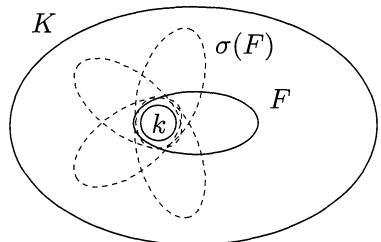
\includegraphics[width=0.45\textwidth]{figs/ch7s6-embed-nongalois.jpg}
\caption{非 Galois 扩张的多个嵌入}
\label{fig:embed-nongalois}
\end{figure}

若 $k\subseteq F$ 是 Galois 的, 所有这些像必重合:

\begin{figure}[h]
\centering
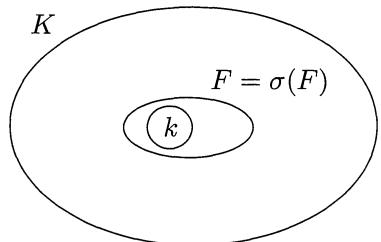
\includegraphics[width=0.45\textwidth]{figs/ch7s6-embed-galois.jpg}
\caption{Galois 扩张的嵌入具有相同的像}
\label{fig:embed-galois}
\end{figure}

当然仍可能有许多方式把 $F$ 嵌入 $K$, 但它们都有相同的像 $F$\footnote{事实上, 当 $K=\overline k$ 时, 这样的嵌入恰有 $[F:k]_s=[F:k]=|\Aut_k(F)|$ 个; 因而对所有 $K\supseteq F$ 也一样.}.

例~\ref{ex:sqrt2-extension} 末尾神秘的评注现在应该有希望清楚了\footnote{这些考虑并没有用到``可分性''; 因此, 比如在特征 $0$ 时, 它们最能传达 Galois 性的直观含义.}. $k$ 的 Galois 扩张是 $\overline{k}$ 中定义良好的子域, 被 $\overline{k}$ 在 $k$ 上的自同构保持. 将此情形与非 Galois 扩张 $\mathbb{Q}\subseteq\mathbb{Q}(\sqrt[3]{2})$ 对比, 后者在 $\overline{\mathbb{Q}}$ 中承认三个不同的嵌入. 例如, 谈论 $\mathbb{Q}(\sqrt{2})$ 与 $\mathbb{Q}(\sqrt[3]{2})$ 的``复合''作为 (比如说) $\mathbb{C}$ 的子域是没有意义的: 依据所取的 $\mathbb{Q}(\sqrt[3]{2})$ 的嵌入, 它可能是也可能不是 $\mathbb{R}$ 的子域. 但谈论两个 Galois 扩张 $k\subseteq F_{1}$, $k\subseteq F_{2}$ 的复合是有意义的, 因为 $F_{1}$ 与 $F_{2}$ 都作为 $\overline{k}$ 的子域\erratumfootnote{根据官方勘误, 原书英文此处修正单复数 (subfields of $\bar{k}$).}定义良好, 故它们的复合 $F_{1}F_{2}$ 与所取的嵌入 $F_{1}\subseteq\overline{k}$, $F_{2}\subseteq\overline{k}$ 无关.

\begin{definition}\label{def:galois-group}
若 $k\subseteq F$ 是 Galois 扩张, 相应的自同构群 $\Aut_k(F)$ 称为该扩张的 \emph{Galois 群}.
\end{definition}

重申一遍, 扩张 $\mathbb{Q}\subseteq\mathbb{Q}(\sqrt[3]{2})$ 不是 Galois 扩张: 正如我们在例~\ref{ex:cube-root-2-not-galois} 中观察到的, $\Aut_{\mathbb{Q}}(\mathbb{Q}(\sqrt[3]{2}))$ 是平凡的 (从而例如定理~\ref{thm:galois-equivalence} 的条件 (3) 不成立).

另一方面, 我们已经遇到过几个 Galois 扩张的例子: 我们在 §\ref{subsec:splitting-fields} 中看到的分裂域的例子都是 Galois 扩张. §\ref{subsec:finite-fields} 的``Galois 域'' (不出所料) 是其素子域的 Galois 扩张, 由定理~\ref{thm:finite-field-classification}. 分圆域 (§\ref{subsec:cyclotomic}) 是 $\mathbb{Q}$ 的 Galois 扩张.

Galois 扩张 $k\subseteq F$ 称为循环, 交换, 等等, 若相应的自同构群 $\Aut_k(F)$ 是循环, 交换, 等等. 例如, $\mathbb{Q}\subseteq\mathbb{Q}(\zeta_{8})$ 是一个交换但非循环的 Galois 扩张 (参见命题~\ref{prop:aut-cyclotomic} 与例~\ref{ex:splitting-x8-1-aut}).

\subsection{Galois 理论基本定理, I}\label{subsec:ft-galois-I}

Galois 理论基本定理本质上是对 Galois 扩张的 Galois 对应给出更完整的描述.

此时我们已经知道:

\begin{itemize}
\item 若 $k\subseteq F$ 是 (有限) Galois 扩张, 则存在一个反包含的双射
\[
\begin{tikzcd}[column sep=3em]
\{\text{中间域 }E:k\subseteq E\subseteq F\} \ar[r,shift left=.7ex] & \{\Aut_k(F)\text{ 的子群}\} \ar[l,shift left=.7ex]
\end{tikzcd},
\]
通过此双射, 中间域 $E$ 对应于 $\Aut_k(F)$ 的子群 $\Aut_E(F)$, 而子群 $G\subseteq\Aut_k(F)$ 对应于不动域 $F^G$.
\item 对每个中间域 $E$,
\[
[F:E]=|\Aut_E(F)|.
\]
进而 $E\subseteq F$ 也是 Galois 扩张 (习题~\ref{ex:intermediate-galois}), 并且
\[
[E:k]=|\Aut_k(F):\Aut_E(F)|;
\]
这由 Lagrange 定理 (推论~II.\ref{cor:lagrange}) 及其域论对应 (命题~\ref{prop:tower-degree}) 推出.
\item 扩张 $k\subseteq E$ 不必是 Galois 的. (再说一遍, $\mathbb{Q}(\sqrt[3]{2})$ 给出了反例, 因为它可以看成 $t^3-2$ 在 $\mathbb{Q}$ 上的分裂域中的中间域.)
\end{itemize}

Galois 对应是双射这一事实可以加强如下:

\begin{theorem}\label{thm:ft-galois-I}
设 $k\subseteq F$ 为 Galois 扩张. Galois 对应是 $k\subseteq F$ 的中间子域格与 $\Aut_k(F)$ 的子群格之间的一个反包含同构.

换言之 (采用引理~\ref{lem:galois-correspondence-inclusion} 的记号), 若 $E_1,E_2$ 是中间域, 而 $G_1,G_2$ 是 $\Aut_k(F)$ 的相应子群, 则 $E_1\cap E_2$ 对应于 $\langle G_1,G_2\rangle$, 而 $E_1E_2$ 对应于 $G_1\cap G_2$.
\end{theorem}

\begin{proof}
这由定理~\ref{thm:galois-equivalence} 与引理~\ref{lem:galois-correspondence-inclusion} 立即推出, 后者给出
\[
\Aut_{E_1E_2}(F)=G_1\cap G_2,\qquad F^{\langle G_1,G_2\rangle}=E_1\cap E_2,
\]
正是所需.
\end{proof}

\index{ziqun@子群(subgroup)!ziyouqunde@自由群的(of a free group)}在此背景下, 人们通常用``竖直''方式描绘域扩张, 并对子群采用平行的记号:
\[
\begin{tikzcd}[row sep=1.2em,column sep=4em]
F \ar[d,no head] & \{e\} \ar[d,no head] \\
E \ar[d,no head] & \Aut_E(F) \ar[d,no head] \\
k & \Aut_k(F)
\end{tikzcd}
\]

定理~\ref{thm:ft-galois-I} 的内容是: Galois 扩张 $k\subseteq F$ 的中间子域格与相应 Galois 群的子群格完全相同.

\begin{example}\label{ex:finite-field-lattice}
对有限域, 这一格的重合本质上已在推论~\ref{cor:finite-field-extension} 与命题~\ref{prop:aut-cyclic-frobenius} 中``手工''证得. 例如, 扩张 $\mathbb{F}_2\subseteq\mathbb{F}_{64}$ 是 Galois 的, 其 Galois 群是循环群 $C_6$, 由 Frobenius 自同构 $\varphi$ 生成. 这两个格是

\begin{figure}[h]
\centering
\begin{tikzcd}[row sep=1.4em,column sep=2em]
& \mathbb F_{64} \ar[dl,no head] \ar[dr,no head] & \\
\mathbb F_8 \ar[dr,no head] & & \mathbb F_4 \ar[dl,no head] \\
& \mathbb F_2 &
\end{tikzcd}
\caption{$\mathbb{F}_2\subseteq\mathbb{F}_{64}$ 的中间域格}
\label{fig:ex613-fields}
\end{figure}

\begin{figure}[h]
\centering
\begin{tikzcd}[row sep=1.4em,column sep=2em]
& \{e\} \ar[dl,no head] \ar[dr,no head] & \\
\{e,\varphi^3\} \ar[dr,no head] & & \{e,\varphi^2,\varphi^4\} \ar[dl,no head] \\
& \{e,\varphi,\varphi^2,\varphi^3,\varphi^4,\varphi^5\} &
\end{tikzcd}
\caption{$\Aut_{\mathbb{F}_2}(\mathbb{F}_{64})\cong C_6$ 的子群格}
\label{fig:ex613-groups}
\end{figure}

\end{example}

定理~\ref{thm:ft-galois-I} 常被用于``由群到域''的方向: 找出一个有限群的子群格本质上是一个组合问题, 而通过 Galois 对应它决定了相应 Galois 扩张的中间子域格.

\begin{example}\label{ex:sqrt2sqrt3-lattice}
扩张 $\mathbb{Q}(\sqrt{2},\sqrt{3})=\mathbb{Q}(\sqrt{2}+\sqrt{3})$ (在例~\ref{ex:sqrt2-sqrt3} 中研究过) 是多项式 $t^4-10t^2+1$ 的分裂域, 因而是 Galois 的. 我们已求得其 Galois 群为 $\mathbb{Z}/2\mathbb{Z}\times\mathbb{Z}/2\mathbb{Z}$; 这个群的格对我们而言已无秘密:

\begin{figure}[h]
\centering
\begin{tikzcd}[row sep=1.4em,column sep=2em]
& \langle(0,0)\rangle \ar[dl,no head] \ar[d,no head] \ar[dr,no head] & \\
\langle(1,0)\rangle \ar[dr,no head] & \langle(1,1)\rangle \ar[d,no head] & \langle(0,1)\rangle \ar[dl,no head] \\
& \mathbb Z/2\mathbb Z\times\mathbb Z/2\mathbb Z &
\end{tikzcd}
\caption{$(\mathbb{Z}/2\mathbb{Z})^2$ 的子群格}
\label{fig:ex614-groups}
\end{figure}

因此中间子域格也同样一目了然:

\begin{figure}[h]
\centering
\begin{tikzcd}[row sep=1.4em,column sep=2em]
& \mathbb Q(\sqrt2,\sqrt3) \ar[dl,no head] \ar[d,no head] \ar[dr,no head] & \\
\mathbb Q(\sqrt2) \ar[dr,no head] & \mathbb Q(\sqrt6) \ar[d,no head] & \mathbb Q(\sqrt3) \ar[dl,no head] \\
& \mathbb Q &
\end{tikzcd}
\caption{$\mathbb{Q}(\sqrt{2},\sqrt{3})$ 的中间子域格}
\label{fig:ex614-fields}
\end{figure}

(中间域由相应子群的生成元决定, 正如在例~\ref{ex:sqrt2-sqrt3} 中所见: 翻转 $\sqrt{3}\mapsto-\sqrt{3}$ 保持 $\mathbb{Q}(\sqrt{2})$ 不动, 等等.) Galois 理论告诉我们没有别的中间域了.
\end{example}

\subsection{Galois 理论基本定理, II}\label{subsec:ft-galois-II}

另一个常见的记号习惯是: 若扩张是 Galois 的, 则用相应的 Galois 群来标注该扩张:
\[
\begin{tikzcd}[row sep=1.1em,column sep=2em]
F \ar[d,no head,"\Aut_E(F)"] \ar[dd,bend right=65,no head,"\Aut_k(F)"'] \\
E \ar[d,no head] \\
k
\end{tikzcd}
\]

例~\ref{ex:cube-root-2-not-galois} 表明扩张 $k\subseteq E$ 未必是 Galois 扩张: $\mathbb{Q}(\sqrt[3]{2})$ 是 $\mathbb{Q}$ 到多项式 $t^3-2$ 的分裂域 (由定理~\ref{thm:galois-equivalence} 的第 (1) 款, 它是 Galois 的) 的中间域, 但如我们所见, 它不是 Galois 的. 该分裂域在 $\mathbb{Q}$ 上的次数为 $6$, 并且是 $\mathbb{Q}(\sqrt[3]{2})$ 的二次扩张. 这其实是典型情形: 每个有限可分扩张都可放大为一个 Galois 扩张 (习题~\ref{ex:galois-closure}).

无论如何, 在一个 Galois 扩张 $k\subseteq F$ 的中间域 $E$ 中, 基域 $k$ 在 $E$ 中的扩张是否为 Galois 扩张这个问题是理论的核心. 讨论的结果将非常漂亮, 而这或许是整个 Galois 理论基本定理中最引人注目的一部分:

\begin{theorem}\label{thm:ft-galois-II}
设 $k\subseteq F$ 为 Galois 扩张, 并设 $E$ 为中间域. 则 $k\subseteq E$ 是 Galois 的, 当且仅当 $\Aut_E(F)$ 在 $\Aut_k(F)$ 中正规; 在此情形存在一个同构
\[
\Aut_k(E)\cong\frac{\Aut_k(F)}{\Aut_E(F)}.
\]
\end{theorem}

关于 $\mathbb{Q}\subseteq\mathbb{Q}(\sqrt[3]{2})$ 的``问题''在于: $t^3-2$ 的分裂域的自同构群是 $S_3$ (我们很快就能验证: 参见例~\ref{ex:cubic-discriminant}). 对应于 $\mathbb{Q}(\sqrt[3]{2})$ 的子群指数为 $3$; 因而 (正如我们所知, 因为我们与 $S_3$ 很熟) 它不是正规的.

Galois 群 $\Aut_k(E)$ 在 Galois 情形将同构于商 $\Aut_k(F)/\Aut_E(F)$, 这一事实不应太过令人惊讶, 因为我们已经知道在任何情形下 $[E:k]$ 都等于 $\Aut_E(F)$ 在 $\Aut_k(F)$ 中的指数, 而该指数在子群正规时等于商的阶. 一般而言, $[E:k]$ 等于 $\Aut_E(F)$ 在 $\Aut_k(F)$ 中左陪集的个数, 而值得为这些陪集——即便在 $k\subseteq E$ 最终不是 Galois 扩张时——给出一个具体的解释.

我们已经知道 $\Aut_E(F)$ 的左陪集个数等于它在 $\Aut_k(F)$ 中的指数, 从而等于 $[E:k]$, 从而等于 $[E:k]_s$ (因为 $k\subseteq E$ 是可分的, 作为可分扩张的子扩张), 因此必然存在一个双射, 介于 $g$ 跑遍 $\Aut_k(F)$ 时的左陪集 $g\Aut_E(F)$ 与 $k$ 的代数闭包中不同的嵌入 $\iota:E\to\overline{k}$ (延拓 $\mathrm{id}_k$) 之间. 我们现在要为此二集合找到一个``有意义的''双射.

固定一个嵌入 $F\subseteq\overline{k}$, 并令 $I$ 为延拓 $k$ 上恒等的嵌入 $\iota:E\hookrightarrow\overline{k}$ 之集合. 把 $k\subseteq E$ 看成一个抽象扩张, 而非把 $E$ 等同于 $F$ 中某个特定的中间域, 是个好主意; 我们能够把 $E$ 看成扩张 $k\subseteq F$ 的中间域这一事实, 仅仅意味着对某个 $\iota\in I$ 有 $\iota(E)\subseteq F$.

如下一般性的观察使情形大为清晰:

\begin{itemize}
\item 对所有 $\iota\in I$, $\iota(E)\subseteq F$.

确实, $k\subseteq E$ 是单的 (有限且可分 $\Longrightarrow$ 单, 命题~\ref{prop:finite-sep-simple}). 若 $E=k(\alpha)$, 则 $\iota$ 由 $\iota(\alpha)$ 决定, 后者必是 $\alpha$ 在 $k$ 上的极小多项式的根. 但 $k\subseteq F$ 是正规的, 并且包含此多项式的某个根 $\iota(\alpha)$; 因此 $F$ 包含所有这些根 (定义~\ref{def:normal-extension}). 也就是说, 对所有 $\iota\in I$ 有 $\iota(\alpha)\in F$, 推出对所有 $\iota\in I$ 有 $\iota(k(\alpha))\subseteq F$.
\item 令 $\iota\in I$, 并令 $g\in\Aut_k(F)$; 则 $g\circ\iota\in I$. 因此 $\Aut_k(F)$ 作用在 $I$ 上.

此处 $g\circ\iota$ 按下述方式理解: 如前所见 $\iota(E)\subseteq F$; 因而 $g$ 限制为一个同态 $\iota(E)\to F$, 而 $g\circ\iota$ 是这个同态与 $\iota$ 的复合.
\end{itemize}

此时宜回顾我们在 §II.\ref{sec:group-actions} 中 (特别是 §II.\ref{subsec:transitive-actions}) 覆盖的群作用素材. 尤其要回忆我们曾能对群在集合上的所有可迁作用进行分类 (命题~II.\ref{prop:transitive-orbits}); 这正是我们的情形:

\begin{itemize}
\item $\Aut_k(F)$ 在 $I$ 上的作用是可迁的.

这由``分裂域的唯一性'' (引理~\ref{lem:splitting-field-unique}) 推出. 事实上, 令 $\iota_1,\iota_2\in I$. $\iota_1(E)$, $\iota_2(E)$ 都包含 $k$, 而 $F$ 是 $k$ 上的分裂域 (定理~\ref{thm:galois-equivalence} 的第 (1) 款); 因此 $F$ 同时是 (对同一多项式) 在 $\iota_1(E)$ 与 $\iota_2(E)$ 上的分裂域. 由引理~\ref{lem:splitting-field-unique}, 存在一个自同构 $g:F\to F$ 延拓同构
\[
\iota_2\circ\iota_1^{-1}:\iota_1(E)\to\iota_2(E).
\]
于是 $g\in\Aut_k(F)$ (因为 $\iota_2\circ\iota_1^{-1}$ 在 $k$ 上限制为恒等), 而 $g$ 在 $\iota_2\circ\iota_1^{-1}$ 上的限制恰恰意味着 $g\circ\iota_1=\iota_2$.
\end{itemize}

现在选取一个 $\iota\in I$, 并用它把 $E$ 等同于 $k\subseteq F$ 的一个中间域. 于是 $\Aut_E(F)=\Aut_{\iota(E)}(F)$ 是 $\Aut_k(F)$ 中那些在 $E=\iota(E)$ 上限制为恒等的元素组成的子群, 亦即 $\iota$ 的稳定子群.

\begin{itemize}
\item 作为 $\Aut_k(F)$-集合, $I$ 同构于 $\Aut_E(F)$ 在 $\Aut_k(F)$ 中左陪集的集合.
\end{itemize}

至此, 这由命题~II.\ref{prop:transitive-orbits} 立即推出.

如所承诺, 我们为这两个集合找到了一个有意义的双射, ``解释''了等式
\[
[E:k]=[E:k]_s=|I|=[\Aut_k(F):\Aut_E(F)],
\]
我们此前已由数值考虑 (即 Lagrange 定理; 参见 §\ref{subsec:ft-galois-I} 的开头) 发现. 进一步, 我们现在可以证明定理~\ref{thm:ft-galois-II} 了.

\begin{proof}[定理~\ref{thm:ft-galois-II} 的证明]
如上所观察, $\Aut_k(F)$ 在 $\iota\in I$ 上的稳定子等于 $\Aut_{\iota(E)}(F)$. 由命题~II.\ref{prop:stabilizer-conjugate}, 不同 $\iota$ 的稳定子彼此共轭; 若 $\Aut_E(F)$ 正规, 则推出对所有 $\iota\in I$
\[
\Aut_{\iota(E)}(F)=\Aut_E(F).
\]
这意味着对所有 $\iota\in I$ 有 $\iota(E)=E$, 因为对 Galois 扩张 $k\subseteq F$ Galois 对应是双射. 由此可知 $k\subseteq E$ 满足定理~\ref{thm:galois-equivalence} 的条件 (6); 因而是 Galois 的.

反过来, 假设 $k\subseteq E$ 是 Galois 的; 由同一条件 (6), 对所有 $\iota\in I$ 有 $\iota(E)=E$. 在 $E=\iota(E)$ 上的限制于是定义了一个同态
\[
\rho:\Aut_k(F)\longrightarrow\Aut_k(E).
\]
这个同态是满的 (因为 $\Aut_k(F)$ 在 $I$ 上的作用可迁), 而其核由那些在 $E$ 上限制为恒等的 $g\in\Aut_k(F)$ 组成, 亦即恰由 $\Aut_E(F)$ 组成. 这表明 $\Aut_E(F)$ 正规, 并且由群的``第一同构定理'' (推论~II.\ref{cor:first-iso}) 建立了所述同构. \qed
\end{proof}

\begin{remark}\label{rmk:galois-cover}
Galois 理论与拓扑中覆叠空间的理论之间有平行之处. 在此类比中, Galois 扩张对应于正则覆叠; 一个扩张的 Galois 群对应于覆叠变换群; 而定理~\ref{thm:ft-galois-II} 对应于如下事实: 正则覆叠被覆叠变换群的一个正规子群作商后仍是正则覆叠.

更一般的 (连通) 覆叠对应于更一般的代数扩张. 一个空间是单连通的, 当且仅当它不容许任何非平凡连通覆叠, 因此这个概念在域论中对应于如下条件: 一个域 $K$ 不容许任何非平凡代数扩张, 亦即 $K$ 是代数闭的. 把一个空间的基本群看成其基覆叠的覆叠变换群, 提示我们应当把代数闭包 $k\subseteq\overline{k}$ 的 Galois 群\footnote{当然, 扩张 $k\subseteq\overline k$ 一般并不是有限的, 因而需要 Galois 理论的无限版本; 参见注~\ref{rmk:infinite-galois}.} 看成域 $k$ 的``基本群''.

在代数几何中, 这个类比被发挥到其自然结论. 代数簇的覆叠映射 $X\to Y$ 决定一个域扩张 $K(Y)\subseteq K(X)$, 其中 $K(X),K(Y)$ 是``有理函数域'' (在仿射情形, 它们恰为相应坐标环的分式域; 参见习题~\ref{ex:rational-functions-localization}). 于是人们可以在不借助拓扑概念 (例如``从 $S^1$ 出发的连续映射'') 的情况下——这些概念在例如正特征时会有问题——用 Galois 理论把基本群之类的概念转移到代数几何环境中.
\end{remark}

\subsection{进一步的注记与例子}\label{subsec:galois-further}

假设 $k\subseteq F$ 与 $k\subseteq K$ 是包含在一个更大的 $k$ 的扩张中的两个有限扩张 (例如, 我们可以在 $k$ 的代数闭包中选取具体的嵌入 $F\subseteq\overline{k}$, $K\subseteq\overline{k}$). 于是我们可以考虑在此更大扩张中 $F,K$ 的复合 $FK$ (参见引理~\ref{lem:galois-correspondence-inclusion}). 很自然地要问 Galois 条件在此运算下如何表现.

\begin{proposition}\label{prop:composite-galois}
假设 $k\subseteq F$ 是 Galois 扩张, 而 $k\subseteq K$ 是任意有限扩张. 则 $K\subseteq KF$ 是 Galois 扩张, 且 $\Aut_K(KF)\cong\Aut_{F\cap K}(F)$.
\end{proposition}

图示如下:

\begin{figure}[h]
\centering
\begin{tikzcd}[row sep=1.1em,column sep=1em]
& KF \ar[dl,no head] \ar[dr,no head,"G"] & \\
F \ar[dr,no head,"G"'] & & K \ar[dl,no head] \\
& F\cap K \ar[d,no head] & \\
& k &
\end{tikzcd}
\caption{复合扩张的 Galois 群}
\label{fig:prop617-composite}
\end{figure}

\begin{proof}
由于 $k\subseteq F$ 是 Galois 的, 它是某个可分多项式 $f(x)\in k[x]\subseteq K[x]$ 的分裂域. $f(x)$ 的根在 $k$ 上生成 $F$, 因而在 $K$ 上生成 $KF$; 换言之, $KF$ 是 $f(x)$ 在 $K$ 上的分裂域, 所以 $K\subseteq KF$ 是 Galois 的.

若 $\sigma:KF\to KF$ 是一个延拓 $K$ 上 (从而在 $k$ 上) 恒等的自同构, 则 $\sigma$ 限制为一个延拓 $k$ 上恒等的同态 $F\to\sigma(F)$. 由于 $k\subseteq F$ 是 Galois 的, $\sigma(F)=F$ (定理~\ref{thm:galois-equivalence} 的 (6)). 因此, ``限制''定义了一个自然的群同态
\[
\rho:\Aut_K(KF)\longrightarrow\Aut_k(F).
\]
我们断言 $\rho$ 是单的. 确实, 依定义每个 $\sigma\in\Aut_K(KF)$ 在 $K$ 上是恒等; 若 $\sigma$ 在 $F$ 上限制为恒等, 则 $\sigma$ 在复合 $KF$ 上是恒等; 也就是说, 在 $\Aut_K(KF)$ 中 $\sigma=\mathrm{id}$.

因此 $\Aut_K(KF)$ 可以等同于 $\Aut_k(F)$ 的一个子群 $G$. 由于每个 $\sigma\in\Aut_K(KF)$ 固定 $K$, 限制 $\rho(\sigma)$ 固定 $F\cap K$; 亦即 $F^G\supseteq F\cap K$. 反过来, 设 $\alpha\in F^G$; 则 $K(\alpha)$ 在 $\Aut_K(KF)$ 的不动域中, 而由于 $K\subseteq KF$ 是 Galois 的 (定理~\ref{thm:galois-equivalence} 的条件 (4)), 此不动域就是 $K$ 本身. 也就是说, $\alpha\in K$, 从而推出 $F^G=F\cap K$. 由命题~\ref{prop:aut-fixed-field-degree}, $G=\Aut_{F\cap K}(F)$, 证毕.
\end{proof}

我们把验证如下事实留给读者: 若 $k\subseteq F$ 与 $k\subseteq K$ 都是 Galois 的, 则 $FK$ 在 $k$ 上也是 Galois 的, 并且 $F\cap K$ 也是 (习题~\ref{ex:composite-intersection-galois}).

\begin{example}\label{ex:cyclotomic-abelian}
我们曾把分圆域 $\mathbb{Q}(\zeta_n)$ 作为 $\mathbb{Q}$ 的扩张来研究; $\mathbb{Q}(\zeta_n)$ 是 $x^n-1$ 的分裂域, 因此这些扩张是 Galois 的; 我们已证明 (命题~\ref{prop:aut-cyclotomic}) $\Aut_{\mathbb{Q}}(\mathbb{Q}(\zeta_n))$ 同构于 $\mathbb{Z}/n\mathbb{Z}$ 的单位群.

现在令 $k$ 为任意特征为零的域. $x^n-1$ 在 $k$ 上的分裂域是 $k$ 与 $\mathbb{Q}(\zeta)$ 的复合 $k(\zeta)$. 由命题~\ref{prop:composite-galois}, 扩张 $k\subseteq k(\zeta)$ 是 Galois 的, 且 $\Aut_k(k(\zeta))$ 同构于 $\mathbb{Z}/n\mathbb{Z}$ 的单位群的一个子群. 特别地, 它是交换的.
\end{example}

前一个例子给出了一类重要的交换 Galois 扩张. 值得注意的是, 如果我们对基域 $k$ 施加某些限制, 就能对所有的循环 Galois 扩张进行分类.

\begin{proposition}\label{prop:kummer}
设 $k\subseteq F$ 是次数为 $m$ 的扩张. 假设 $k$ 包含一个本原 $m$ 次单位根, 且 $\Char k$ 不整除 $m$. 则 $k\subseteq F$ 是 Galois 且循环的, 当且仅当 $F=k(\delta)$, 其中 $\delta^m\in k$.
\end{proposition}

也就是说, 在关于 $k$ 的上述假设下, $k$ 的循环 Galois 扩张恰为形如 $k\subseteq k(\sqrt[m]{c})$ ($c\in k$) 的那些. 这是 Kummer 理论的一部分, 它是研究交换扩张的基本工具. 命题~\ref{prop:kummer} 将成为我们把 Galois 理论应用于多项式方程可解性的一个关键要素\footnote{我们将在 §\ref{subsec:radical-solvability} 中应用这一结果; 为方便起见, 那里将取 $\Char k=0$.}.

\begin{proof}
令 $\zeta\in k$ 为一个本原 $m$ 次单位根.

首先假设 $F=k(\delta)$, 其中 $\delta^m=c\in k$. 于是多项式 $x^m-c$ 的全部 $m$ 个根
\[
\delta,\zeta\delta,\zeta^2\delta,\ldots,\zeta^{m-1}\delta
\]
都在 $F$ 中, 并且 $F$ 由它们生成; 因此 $F$ 是此可分多项式 (因为 $\Char k$ 不整除 $m$) 在 $k$ 上的分裂域; 从而 (定理~\ref{thm:galois-equivalence} 的第 (1) 款) $k\subseteq F$ 是 Galois 的. 注意, 由于 $F=k(\delta)$ 在 $k$ 上的次数为 $m$, 且 $\delta$ 是 $x^m-c$ 的根, 故推出多项式 $x^m-c$ 是不可约的\erratumfootnote{根据官方勘误, 原书在此处补充说明: ``注意, 由于 $F=k(\delta)$ 在 $k$ 上的次数为 $m$, 且 $\delta$ 是 $x^m-c$ 的根, 故推出多项式 $x^m-c$ 是不可约的 (Note that since $F=k(\delta)$ has degree $m$ over $k$, and $\delta$ is a root of $x^m-c$, it follows that the polynomial $x^m-c$ is irreducible)''.}.

为看出 $\Aut_k(F)$ 是循环的, 注意每个 $\varphi\in\Aut_k(F)$ 由 $\varphi(\delta)$ 决定, 后者必是 $x^m-c$ 的一个根; 因此 $\varphi(\delta)=\zeta^i\delta$ 对某个 $i$ 成立, 此 $i$ 模 $m$ 确定. 这定义了 $\Aut_k(F)$ 到 $\mathbb{Z}/m\mathbb{Z}$ 的一个同构, 一如直接验证所示.

反过来, 假设 $k\subseteq F$ 是 Galois 的且 $\Aut_k(F)$ 循环, 由 $\varphi$ 生成. 自同构 $\varphi^i$ ($i=0,\ldots,m-1$) 两两不同; 因此它们在 $F$ 上线性无关 (习题~\ref{ex:aut-linearly-independent}). 于是存在 $\alpha\in F$ 使得\footnote{这个表达式称为 Lagrange 预解式.}
\[
\delta:=\alpha+\zeta^{-1}\varphi(\alpha)+\cdots+\zeta^{-(m-2)}\varphi^{m-2}(\alpha)+\zeta^{-(m-1)}\varphi^{m-1}(\alpha)\neq 0.
\]
注意
\[
\varphi(\delta)=\varphi(\alpha)+\zeta^{-1}\varphi^2(\alpha)+\cdots+\zeta^{-(m-2)}\varphi^{m-1}(\alpha)+\zeta^{-(m-1)}\alpha=\zeta\delta
\]
(因为 $\zeta\in k$, 故 $\varphi(\zeta)=\zeta$). 这意味着 $\delta$ 不被 $\Aut_k(F)$ 的任何非单位元固定; 也就是说, $\Aut_{k(\delta)}(F)=\{e\}$; 也就是说, $k(\delta)=F$. 进一步,
\[
\varphi(\delta^m)=(\varphi(\delta))^m=\zeta^m\delta^m=\delta^m;
\]
也就是说, $\delta^m$ 被 $\varphi$ 固定, 从而被整个 $\Aut_k(F)$ 固定. 由于 $k\subseteq F$ 是 Galois 的, 这推出 $\delta^m\in k$ (定理~\ref{thm:galois-equivalence} 的条件 (4)). 也就是说, $\delta$ 满足所述条件.
\end{proof}

\subsection*{习题}
\phantomsection
\addcontentsline{toc}{subsection}{习题}

\begin{prob}\label{ex:galois-ft-lemma}
证明引理~\ref{lem:galois-correspondence-inclusion}. [§\ref{subsec:galois-correspondence}]
\end{prob}

\begin{prob}\label{ex:quadratic-galois}
证明特征不为 $2$ 的域的二次扩张是 Galois 的.
\end{prob}

\begin{prob}\label{ex:intermediate-galois}
$\triangleright$ 设 $k\subseteq F$ 为 Galois 扩张, 并设 $E$ 为中间域. 证明 $E\subseteq F$ 是 Galois 扩张. [§\ref{subsec:ft-galois-I}]
\end{prob}

\begin{prob}\label{ex:galois-closure}
$\triangleright$ 设 $k\subseteq E$ 为有限可分扩张. 证明 $E$ 可以等同于 $k$ 的某个 Galois 扩张 $k\subseteq F$ 的中间域.

事实上, 证明存在最小的这样的扩张 $k\subseteq F$, 其意义是: 若 $k\subseteq E\subseteq K$, 其中 $k\subseteq K$ 为 Galois 的, 则存在 $F$ 到 $K$ 的一个嵌入, 它在 $E$ 上是恒等. (扩张 $k\subseteq F$ 是扩张 $k\subseteq E$ 的 Galois 闭包. 它在同构意义下显然唯一确定.) [§\ref{subsec:ft-galois-II}, \ref{ex:simple-gen-aut}]
\end{prob}

\begin{prob}\label{ex:simple-gen-aut}
我们已证明 (命题~\ref{prop:finite-sep-simple}) 所有有限可分扩张 $k\subseteq E$ 都是单的. 设 $k\subseteq F$ 是 $k\subseteq E$ 的一个 Galois 闭包 (习题~\ref{ex:galois-closure}). 对 $\alpha\in E$, 证明 $E=k(\alpha)$ 当且仅当 $\alpha$ 被所有 $\sigma\in\Aut_k(F)\setminus\Aut_E(F)$ 移动.
\end{prob}

\begin{prob}\label{ex:sqrt2sqrt2-galois}
$\bullet$ 证明 $\mathbb{Q}\subseteq\mathbb{Q}(\sqrt{2+\sqrt{2}})$ 是 Galois 的, 且具有循环 Galois 群. (参见习题~\ref{ex:xi-sqrt2-sqrt2}.)

$\bullet$ 证明 $\mathbb{Q}\subseteq\mathbb{Q}(\sqrt{3+\sqrt{5}})$ 是 Galois 的, 且其 Galois 群同构于 $(\mathbb{Z}/2\mathbb{Z})\times(\mathbb{Z}/2\mathbb{Z})$.

$\bullet$ 证明 $\mathbb{Q}\subseteq\mathbb{Q}(\sqrt{1+\sqrt{2}})$ 不是 Galois 的, 并计算其 Galois 闭包 $\mathbb{Q}\subseteq F$. 证明 $\Aut_{\mathbb{Q}}(F)\cong D_8$. (利用习题~IV.\ref{ex:order-8}.)
\end{prob}

\begin{prob}\label{ex:finite-field-galois-degree}
设 $p>0$ 为素数, 并设 $d\mid e$ 为正整数, 于是存在扩张 $F_{p^d}\subseteq F_{p^e}$. 证明 $\Aut_{F_{p^d}}F_{p^e}$ 是循环的, 并描述这个群的一个生成元. (这推广了命题~\ref{prop:aut-cyclic-frobenius}; 用 Galois 理论.)
\end{prob}

\begin{prob}\label{ex:prime-degree-galois}
设 $k\subseteq F$ 为次数 $n$ 的 Galois 扩张, 并设 $E$ 为中间域. 假设 $[E:k]$ 是整除 $n$ 的最小素数. 证明 $k\subseteq E$ 是 Galois 的.
\end{prob}

\begin{prob}\label{ex:degree75-galois}
设 $k\subseteq F$ 为次数 $75$ 的 Galois 扩张. 证明存在中间域 $E$, 满足 $k\subsetneq E\subsetneq F$, 使得扩张 $k\subseteq E$ 是 Galois 的.
\end{prob}

\begin{prob}\label{ex:normalizer-autE}
设 $k\subseteq F$ 为 Galois 扩张, 并设 $E$ 为中间域. 证明 $\Aut_E(F)$ 在 $\Aut_k(F)$ 中的正规化子恰为那些满足 $\sigma(E)\subseteq E$ 的 $\sigma\in\Aut_k(F)$ 之集合.

利用此给出如下事实的另一个证明: $E$ 在 $k$ 上 Galois, 当且仅当 $\Aut_E(F)$ 在 $\Aut_k(F)$ 中正规.
\end{prob}

\begin{prob}\label{ex:galois-transitive}
设 $k\subseteq E$ 与 $E\subseteq F$ 为 Galois 扩张.

$\bullet$ 找出一个例子说明 $k\subseteq F$ 未必是 Galois 的.

$\bullet$ 证明若每个 $\sigma\in\Aut_k(E)$ 都是某个 $\Aut_k(F)$ 的元素的限制, 则 $k\subseteq F$ 是 Galois 的.
\end{prob}

\begin{prob}\label{ex:composite-nonisomorphic}
找出两个代数扩张 $k\subseteq F$, $k\subseteq K$ 以及嵌入 $F\subseteq\overline{k}$, $\sigma_1:K\subseteq\overline{k}$, $\sigma_2:K\subseteq\overline{k}$ (延拓 $k\subseteq\overline{k}$), 使得复合 $F\sigma_1(K)$, $F\sigma_2(K)$ 不同构.

证明若 $F$ 与 $K$ 都在 $k$ 上 Galois, 则不存在这样的例子.
\end{prob}

\begin{prob}\label{ex:composite-intersection-galois}
$\triangleright$ 设 $k\subseteq F$ 与 $k\subseteq K$ 为 Galois 扩张, 并假设 $F$ 与 $K$ 是一个更大域的子域. 证明 $k\subseteq FK$ 与 $k\subseteq F\cap K$ 都是 Galois 扩张. [§\ref{subsec:galois-further}, §\ref{subsec:radical-solvability}]
\end{prob}

\begin{prob}\label{ex:aut-linearly-independent}
$\triangleright$ 设 $k\subseteq F$ 为域扩张, 并设 $\varphi_1,\ldots,\varphi_m\in\Aut_k(F)$ 为两两不同的自同构. 证明 $\varphi_1,\ldots,\varphi_m$ 在 $F$ 上线性无关. (回收/改编习题~VI.\ref{ex:distinct-eigenvectors-independent} 的提示.) [§\ref{subsec:galois-further}, \ref{ex:hilbert90-multiplicative}, §\hyperref[subsec:7.6-group-cohomology]{IX.7.6}]
\end{prob}

\begin{prob}\label{ex:norm-trace-product}
设 $k\subseteq F$ 为 Galois 扩张, 并设 $\alpha\in F$. 证明
\[
N_{k\subseteq F}(\alpha)=\prod_{\sigma\in\Aut_k(F)}\sigma(\alpha),\qquad \tr_{k\subseteq F}(\alpha)=\sum_{\sigma\in\Aut_k(F)}\sigma(\alpha).
\]
(习题~\ref{ex:norm-trace-embeddings}.)
\end{prob}

\begin{prob}\label{ex:hilbert90-multiplicative}
$\triangleright$ 设 $k\subseteq F$ 为次数 $d$ 的循环 Galois 扩张, 并设 $\varphi$ 为 $\Aut_k(F)$ 的一个生成元. 令 $\alpha\in F$ 为满足 $N_{k\subseteq F}(\alpha)=1$ 的元素.

$\bullet$ 证明自同构 $\mathrm{id}_F,\varphi,\ldots,\varphi^{d-1}$ 在 $F$ 上线性无关. (习题~\ref{ex:aut-linearly-independent}.)

$\bullet$ 证明存在 $\gamma\in F$ 使得
\[
\beta:=\gamma+\alpha\varphi(\gamma)+\alpha\varphi(\alpha)\varphi^2(\gamma)+\cdots+\alpha\varphi(\alpha)\cdots\varphi^{d-2}(\alpha)\varphi^{d-1}(\gamma)\neq 0.
\]

$\bullet$ 证明 $\alpha\varphi(\alpha)\varphi^2(\alpha)\cdots\varphi^{d-1}(\alpha)\varphi^d(\gamma)=\gamma$, 并推出 $\alpha=\beta/\varphi(\beta)$.

结合习题~\ref{ex:norm-trace-aut} 的结果, 结论是: 上述循环 Galois 扩张的元素 $\alpha$ 具有范数 $1$, 当且仅当存在 $\beta$ 使得 $\alpha=\beta/\varphi(\beta)$.

这就是 Hilbert 的定理 90 (Hilbert 的 Zahlbericht 中的第 90 个定理, 这是一份由德国数学会委托的、关于十九世纪末数论状况的报告). [\ref{ex:hilbert90-additive}, §\hyperref[subsec:7.6-group-cohomology]{IX.7.6}, IX.\ref{ex:7.18}]
\end{prob}

\begin{prob}\label{ex:hilbert90-kummer}
习题~\ref{ex:hilbert90-multiplicative} 应当让读者回想起命题~\ref{prop:kummer} 的证明, 这是有原因的. 假设 $k\subseteq F$ 是次数 $m$ 的循环 Galois 扩张, 且 $k$ 包含一个本原 $m$ 次单位根 $\zeta$. 利用 Hilbert 的定理 90 证明 $F=k(\delta)$, 其中 $\delta^m\in k$, 从而重新得到命题~\ref{prop:kummer} 所述结论的一个方向. (提示: $N_{k\subseteq F}(\zeta^{-1})$ 是什么?)

这里需要的 Hilbert 定理 90 的情形归功于 Kummer.
\end{prob}

\begin{prob}\label{ex:hilbert90-rational}
利用 Hilbert 的定理 90 找出方程 $a^2+b^2d=1$ 的所有有理根 $a,b$, 其中 $d$ 是非平方的正整数. (提示: $a^2+b^2d$ 等于 $N_{\mathbb{Q}\subseteq\mathbb{Q}(\sqrt{-d})}(a+b\sqrt{-d})$; 参见习题~\ref{ex:norm-alpha}.)
\end{prob}

\begin{prob}\label{ex:hilbert90-additive}
$\neg$ 设 $k\subseteq F$ 为次数 $d$ 的循环 Galois 扩张, 并设 $\varphi$ 为 $\Aut_k(F)$ 的一个生成元. 令 $\alpha\in F$ 为满足 $\tr_{k\subseteq F}(\alpha)=0$ 的元素. 证明 Hilbert 定理 90 的一个``加性版本'':

$\bullet$ 证明存在 $\gamma\in F$ 使得 $\tr_{k\subseteq F}(\gamma)\neq 0$.

$\bullet$ 盯着表达式
\[
\alpha\varphi(\gamma)+(\alpha+\varphi(\alpha))\varphi^2(\gamma)+\cdots+(\alpha+\varphi(\alpha)+\cdots+\varphi^{d-2}(\alpha))\varphi^{d-1}(\gamma)
\]
看.

$\bullet$ 证明存在 $\beta\in F$ 使得 $\alpha=\beta-\varphi(\beta)$.

结合习题~\ref{ex:norm-trace-aut}, 这说明上述循环 Galois 扩张的元素 $\alpha$ 具有迹 $0$, 当且仅当存在 $\beta$ 使得 $\alpha=\beta-\varphi(\beta)$. 一个应用见习题~\ref{ex:cyclic-char-p-artin-schreier}. [习题~\ref{ex:cyclic-char-p-artin-schreier}]
\end{prob}

\section{Galois 理论应用简述}
\label{sec:galois-applications}

Galois 理论是一个无处不在的工具, 应用极其广泛. 我们既没有能力也没有篇幅在这本书里对 Galois 理论的应用做一个充分的综述, 但即使本节回顾的这几个例子, 也足以让人感受到它相当大的威力.

\subsection{代数基本定理}
\label{subsec:ft-algebra}

定理~\ref{thm:ft-galois-II} 与一点点群论, 本质上就是给出代数基本定理的一个纯代数证明所需要的全部\footnote{其实我们稍微作弊了一点, 因为中间值定理也会在幕后用到. 这并不太令人意外: $\mathbb{R}$ 的完备性必须在某个地方进入证明.}, 这个证明我们早在 §V.\ref{subsec:irred-CRQ} 就许诺过了.

\begin{theorem}\label{thm:ft-algebra}
$\mathbb{C}$ 是代数闭的.
\end{theorem}

\begin{proof}
设 $f(x)\in\mathbb{C}[x]$ 为一个非常数多项式; 我们要证明 $f(x)$ 在 $\mathbb{C}$ 中有根. 注意若 $f(x)$ 在 $\mathbb{C}$ 中没有根, 则 $f(x)\overline{f(x)}\in\mathbb{R}[x]$ 也没有根 (其中 $\overline{f(x)}$ 表示把 $f(x)$ 的系数取复共轭所得的多项式); 也就是说, 我们不妨假设 $f(x)$ 有实系数. 令 $F$ 为 $f(x)$ 在 $\mathbb{R}$ 上的一个分裂域; 将 $F$ 嵌入 $\mathbb{R}$ 的一个代数闭包中 (我们``还不知道'' $\mathbb{C}$ 是代数闭的!), 并考虑扩张
\[
\mathbb{R}\subseteq F(i).
\]
这个扩张是 Galois 的: 它是多项式 $f(x)(x^2+1)$ 的无平方因子部分\footnote{即取该多项式的每个不可约因子, 其幂次恰好为 $1$. 在完美域上, 无平方因子多项式显然可分.}的分裂域. 令 $G=\Aut_{\mathbb{R}}(F(i))$.

由西罗 I (定理~IV.\ref{thm:sylow-I}), $G$ 有一个 $2$-西罗子群 $H$. 指数 $[G:H]$ 为奇数, 因此它对应于一个有限可分扩张 $\mathbb{R}\subseteq E$, 满足 $[E:\mathbb{R}]$ 为奇数. 然而, $\mathbb{R}$ 上每个奇次多项式都有实根 (习题~V.\ref{ex:odd-degree-ivt}, 它只用到初等的微积分), 由此推出 $\mathbb{R}\subseteq E$ 是平凡的 (习题~\ref{ex:no-irred-no-sep-extension}).

因此 $[G:H]=1$, 说明 $G$ 是一个 $2$-群. 由于 $\mathbb{C}=\mathbb{R}(i)\subseteq F(i)$, Galois 扩张 (也是 Galois 的) $\mathbb{C}\subseteq F(i)$ 的 Galois 群是 $G$ 的一个子群; 因此它是一个 $2$-群: $\lvert\Aut_{\mathbb{C}}(F(i))\rvert=2^n$ 对某个 $n\ge 0$.

现在回忆 (命题~IV.\ref{prop:p-subgroup-all-sizes}), 对每个素数 $p$, 阶为 $p^n$ 的群都含有阶为 $p^m$ 的子群, 其中 $0\le m\le n$. 特别地, 若 $n\ge 1$, 则 $\Aut_{\mathbb{C}}(F(i))$ 含有一个阶为 $2^{n-1}$ 的子群, 它通过 Galois 对应对应于 $\mathbb{C}$ 的一个二次扩张. 然而 $\mathbb{C}$ 没有二次扩张, 因为 $\mathbb{C}[x]$ 中不存在不可约的二次多项式 (再次见习题~\ref{ex:no-irred-no-sep-extension}).

这个矛盾说明 $n=0$; 也就是说, $\Aut_{\mathbb{C}}(F(i))$ 必然是平凡的. 这就证明了 $F(i)=\mathbb{C}$, 特别地 $\mathbb{C}$ 含有 $f(x)$ 的根.
\end{proof}

也可以把论证进一步简化, 绕过西罗定理的使用, 代价只是长度略有增加. 但是, 在第四章花了那么大力气证明西罗定理之后, 我们又何必去绕过它呢?

\subsection{正 \texorpdfstring{$n$}{n} 边形的作图}
\label{subsec:constructible-ngons}

我们最后一次回到正 $n$ 边形作图的问题. 较为简单的考虑已经给出了 $n$ 必须满足的约束条件, 正 $n$ 边形要可作图, 这些条件必不可少: 若 $n=p$ 为素数, 我们已经发现 $p-1$ 必须是 $2$ 的幂 (§\ref{subsec:famous-impossibilities}); 对任意的 $n$ 这个结果被加强为 $\varphi(n)$ 是 $2$ 的幂, 见 §\ref{subsec:cyclotomic} (而一个更明确的条件由习题~\ref{ex:regular-n-gon-constructible} 给出). 但这些全都是``否定性''的结果: 我们至今尚未证明, 如果 $\varphi(n)$ 是 $2$ 的幂, 那么正 $n$ 边形就真的可作图. 这正是 Galois 理论出场的地方.

\begin{proposition}\label{prop:constructible-tower}
设 $k\subseteq F$ 为 Galois 扩张, 并设 $[F:k]=p^r$, 其中 $p$ 为某个素数, $r\ge 0$. 则存在中间域
\[
k=E_0\subseteq E_1\subseteq E_2\subseteq\cdots\subseteq E_r=F
\]
使得对 $i=1,\ldots,r$ 有 $[E_i:E_{i-1}]=p$.
\end{proposition}

\begin{proof}
由于对 Galois 扩张 Galois 对应是双射的 (定理~\ref{thm:galois-equivalence} 的第 (5) 款), 这个结论直接从如下事实推出: 阶为 $p^r$ (其中 $p$ 为素数) 的群有一条由 $p$-子群构成的完全子群列; 例如可参见定理~IV.\ref{thm:sylow-II} 之后的讨论.
\end{proof}

\begin{theorem}\label{thm:regular-n-gon}
正 $n$ 边形可用直尺与圆规作图, 当且仅当 $\varphi(n)$ 是 $2$ 的幂.
\end{theorem}

\begin{proof}
如上所忆, 我们已经建立了 ``$\Longrightarrow$'' 方向.

对反方向, 假设对某个 $r$ 有 $\varphi(n)=2^r$. 扩张 $\mathbb{Q}\subseteq\mathbb{Q}(\zeta_n)$ 是 Galois 的 (它是分圆多项式 $\Phi_n(x)$ 的分裂域), 其阶为 $[\mathbb{Q}(\zeta_n):\mathbb{Q}]=\varphi(n)=2^r$ (命题~\ref{prop:cyclotomic-irred}). 命题~\ref{prop:constructible-tower} 表明定理~\ref{thm:constructible-quadratic} 所给出的条件得到满足, 从而 $\zeta_n$ 可作图, 如所求.
\end{proof}

例如 $\varphi(17)=16=2^4$; $\mathbb{Q}(\zeta_{17})$ 在 $\mathbb{Q}$ 上的 Galois 群同构于 $(\mathbb{Z}/17\mathbb{Z})^*$ (由命题~\ref{prop:aut-cyclotomic}), 因此 (定理~IV.\ref{thm:finite-subfield-cyclic}) 它是循环群, 阶为 $16$. $(\mathbb{Z}/17\mathbb{Z})^*$ 的一个生成元是 $[6]_{17}$; 由此可知 $\Aut_{\mathbb{Q}}(\mathbb{Q}(\zeta_{17}))$ 由自同构 $\sigma$ 生成, 其中 $\sigma$ 定义为 $\zeta_{17}\mapsto\zeta_{17}^6$. 子群
\[
\{e\}\subseteq\langle\sigma^8\rangle\subseteq\langle\sigma^4\rangle\subseteq\langle\sigma^2\rangle\subseteq\langle\sigma\rangle
\]
通过 Galois 对应对应于一列扩张
\[
\mathbb{Q}\subseteq\mathbb{Q}(\zeta_{17})^{\langle\sigma^2\rangle}\subseteq\mathbb{Q}(\zeta_{17})^{\langle\sigma^4\rangle}\subseteq\mathbb{Q}(\zeta_{17})^{\langle\sigma^8\rangle}\subseteq\mathbb{Q}(\zeta_{17}).
\]
运用我们现在所知的知识, 来看一看如何确定第一个扩张 (即 $\sigma^2$ 的固定域) 的一个生成元, 是很有教益的. 令 $\zeta=\zeta_{17}$. 作为 $\mathbb{Q}$-向量空间, $\mathbb{Q}(\zeta)$ 由 $\zeta,\zeta^2,\ldots,\zeta^{16}$ 生成. 为找出 $\sigma^2$ 的固定域, 写出一个 $\mathbb{Q}(\zeta)$ 的一般元素:
\[
\begin{aligned}&a_1\zeta+a_2\zeta^2+a_3\zeta^3+a_4\zeta^4+a_5\zeta^5+a_6\zeta^6+a_7\zeta^7+a_8\zeta^8\\
&+a_9\zeta^9+a_{10}\zeta^{10}+a_{11}\zeta^{11}+a_{12}\zeta^{12}+a_{13}\zeta^{13}+a_{14}\zeta^{14}+a_{15}\zeta^{15}+a_{16}\zeta^{16};
\end{aligned}
\]
由于 $\sigma^2(\zeta)=(\zeta^6)^6=\zeta^{36}=\zeta^2$, 它在 $\sigma^2$ 作用下的像为
\[
\begin{aligned}&a_1\zeta^2+a_2\zeta^4+a_3\zeta^6+a_4\zeta^8+a_5\zeta^{10}+a_6\zeta^{12}+a_7\zeta^{14}+a_8\zeta^{16}\\
&+a_9\zeta+a_{10}\zeta^3+a_{11}\zeta^5+a_{12}\zeta^7+a_{13}\zeta^9+a_{14}\zeta^{11}+a_{15}\zeta^{13}+a_{16}\zeta^{15}.
\end{aligned}
\]
这个元素被 $\sigma^2$ 固定, 当且仅当$a_1=a_2=a_4=a_8=a_{16}=a_{15}=a_{13}=a_9$ 且 $a_3=a_6=a_{12}=a_7=a_{14}=a_{11}=a_5=a_{10}$; 由此可知 $\sigma^2$ 的固定域由
\[
\delta_1:=\zeta+\zeta^2+\zeta^4+\zeta^8+\zeta^{16}+\zeta^{15}+\zeta^{13}+\zeta^9
\]
生成, 而同一个固定域也由
\[
\zeta^3+\zeta^6+\zeta^{12}+\zeta^7+\zeta^{14}+\zeta^{11}+\zeta^5+\zeta^{10}=-1-\delta_1
\]
生成 (记住 $\zeta$ 是 $\Phi_{17}(x)=x^{16}+\cdots+x+1$ 的根). 如图所见,

\begin{figure}[ht]
\centering
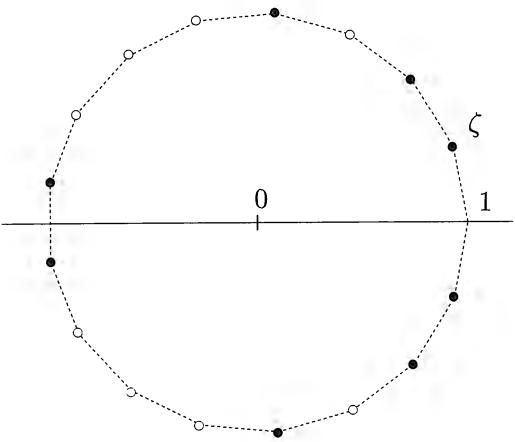
\includegraphics[width=0.55\textwidth]{figs/ch7s7-fig17roots.jpg}
\caption{正 $17$ 边形的 $17$ 次单位根. 黑点标记的根之和为 $\delta_1$; 白点标记的根之和为 $-1-\delta_1$.}
\label{fig:ch7s7-fig17roots}
\end{figure}

\noindent 黑点标记的根之和为 $\delta_1$; 白点标记的根之和为 $-1-\delta_1$. 理论告诉我们 $\delta_1$ 在 $\mathbb{Q}$ 上的次数为 $2$, 从而 $\delta_1^2$ 可写成 $1$ 与 $\delta_1$ 的有理系数线性组合. 确实, 用笔, 纸和一点耐心 (以及关系 $\zeta^{17}=1$) 可以得到
\[
\begin{aligned}\delta_1^2&=(\zeta+\zeta^2+\zeta^4+\zeta^8+\zeta^{16}+\zeta^{15}+\zeta^{13}+\zeta^9)^2\\
&=3(\zeta+\zeta^2+\zeta^4+\zeta^8+\zeta^{16}+\zeta^{15}+\zeta^{13}+\zeta^9)\\
&\quad+4(\zeta^3+\zeta^6+\zeta^{12}+\zeta^7+\zeta^{14}+\zeta^{11}+\zeta^5+\zeta^{10})+8.
\end{aligned}
\]
而第二个括号中的和等于 $-1-\delta_1$ (因为全部 $16$ 个非 $1$ 的 $17$ 次单位根之和为 $-1$); 于是
\[
\delta_1^2=3\delta_1+4(-1-\delta_1)+8=-\delta_1+4.
\]
因此 $\delta_1^2+\delta_1-4=0$. 解出 $\delta_1$ (注意 $\delta_1>0$, 因为 $0$ 右侧的黑点多于左侧的) 得
\[
\delta_1=\frac{-1+\sqrt{17}}{2}.
\]
于是我们可以轻易构造 $\delta_1$. 对其它扩张施以同样的程序可以产生 $\delta_2,\delta_3$, 最后得到 $\zeta_{17}$, 其实部就是 §\ref{subsec:famous-impossibilities} 末尾给出的那个复杂表达式.

\subsection{对称函数基本定理}
\label{subsec:sym-funcs}

设 $t_1,\ldots,t_n$ 为不定元. 多项式
\[
P_n(x):=(x-t_1)\cdots(x-t_n)\in\mathbb{Z}[t_1,\ldots,t_n][x]
\]
具有普遍性: 系数在某个 (比如说) 整环中的、次数 $n$ 的每一个首一多项式\erratumfootnote{根据官方勘误, 补充限定为首一多项式 (every monic polynomial of degree $n$).}, 都可以通过适当地指定 $t_1,\ldots,t_n$ (可能在某个更大的环中) 从 $P_n(x)$ 得到 (习题~\ref{ex:universal-poly-specialize}). 展开式
\[
P_n(x)=x^n-s_1(t_1,\ldots,t_n)x^{n-1}+s_2(t_1,\ldots,t_n)x^{n-2}-\cdots+(-1)^n s_n(t_1,\ldots,t_n)
\]
的系数 (相差一个符号) 就是 $t_1,\ldots,t_n$ 的初等对称函数. 例如, 对 $n=3$,
\[
\begin{aligned}
s_1(t_1,t_2,t_3)&=t_1+t_2+t_3,\\
s_2(t_1,t_2,t_3)&=t_1t_2+t_1t_3+t_2t_3,\\
s_3(t_1,t_2,t_3)&=t_1t_2t_3.
\end{aligned}
\]
函数 $s_i(t_1,\ldots,t_n)$ 是对称的, 意思是它们在置换 $t_1,\ldots,t_n$ 下不变 (因为 $P_n(x)$ 不变); 它们之所以是初等的, 全凭如下重要结果, 而借助 Galois 理论, 这个结果有一个特别简单的证明.

\begin{theorem}[对称函数基本定理]\label{thm:sym-funcs}
设 $K$ 为一个域, 并设 $\varphi\in K(t_1,\ldots,t_n)$. 则 $\varphi$ 是对称的, 当且仅当它是初等对称函数 $s_1,\ldots,s_n$ 的有理函数 (系数在 $K$ 中).
\end{theorem}

这里我们把 $s_i$ 无歧义地视为 $K[t_1,\ldots,t_n]$ 中的元素, 因为 $\mathbb{Z}$ 在环范畴中是初始对象.

\begin{proof}
令 $F=K(t_1,\ldots,t_n)$, 并令 $k=K(s_1,\ldots,s_n)$ 为初等对称函数在 $K$ 上生成的子域.

于是 $F$ 是可分多项式 $P_n(x)$ 在 $k$ 上的分裂域. 特别地 $k\subseteq F$ 是 Galois 扩张, 且
\[
\lvert\Aut_k(F)\rvert=[F:k]\le n!
\]
(引理~\ref{lem:splitting-field-unique}). 对称群 $S_n$ 通过置换 $t_1,\ldots,t_n$ 在 $F$ 上 (忠实地) 作用, 而这个作用在每个 $s_i$ 上都是恒等, 因为 $s_i$ 对称; 因此 $S_n$ 可以等同于 $\Aut_k(F)$ 的一个子群. 但 $\lvert S_n\rvert=n!$, 所以推出 $\Aut_k(F)=S_n$.

由于 $k\subseteq F$ 是 Galois 的, 我们得到 $k=F^{S_n}$. 这精确地说就是: 若 $\varphi\in K(t_1,\ldots,t_n)$, 则 $\varphi$ 在 $S_n$ 对 $t_1,\ldots,t_n$ 的作用下的不变性, 当且仅当 $\varphi\in k=K(s_1,\ldots,s_n)$, 这正是所要证的结论.
\end{proof}

定理~\ref{thm:sym-funcs} 的结论并不难进一步加强, 来证明每个对称多项式事实上都是初等对称函数的多项式. 注意上面证明中的推理等价于如下结果, 它值得单独记下来:

\begin{lemma}\label{lem:sym-funcs-galois}
设 $K$ 为域, $t_1,\ldots,t_n$ 为不定元, $s_1,\ldots,s_n$ 为 $t_1,\ldots,t_n$ 上的初等对称函数. 则扩张
\[
K(s_1,\ldots,s_n)\subseteq K(t_1,\ldots,t_n)
\]
是 Galois 的, 其 Galois 群为 $S_n$.
\end{lemma}

这个结果与 Cayley 定理 (定理~II.\ref{thm:cayley}) 立刻给出:

\begin{corollary}\label{cor:every-finite-group-galois}
设 $G$ 为有限群. 则存在 Galois 扩张 $k\subseteq F$ 使得 $\Aut_k(F)\cong G$.
\end{corollary}

\begin{proof}
习题~\ref{ex:every-finite-group-galois}.
\end{proof}

\index{ni Galois wenti@逆 Galois 问题(inverse Galois problem)}我们还不知道在推论~\ref{cor:every-finite-group-galois} 中能否取 $k=\mathbb{Q}$. 上面暗示的证明把 $k$ 实现为一个相当大的域, 并且完全不清楚如何从这个域``下降''到 $\mathbb{Q}$. 这就是反 Galois 问题, 一个当前研究的课题. 读者可以体会到这个问题的难度: 即使对所有的 $n$ 把 $S_n$ 实现为 $\mathbb{Q}$ 上的 Galois 群也并不容易, 尽管如下事实成立——对每个 $n$, 在 $\mathbb{Z}[x]$ 中有无穷多个 $n$ 次多项式, 其分裂域在 $\mathbb{Q}$ 上的 Galois 群为 $S_n$ (见例~\ref{ex:prime-degree-sp} 与习题~\ref{ex:prime-degree-sp-infinite} 中 $n=p$ 为素数的情形). 如果你想随身带一个好记的例子, Schur 在 1931 年证明了, ``截断指数''
\[
1+x+\frac{x^2}{2!}+\frac{x^3}{3!}+\cdots+\frac{x^n}{n!}
\]
的分裂域在 $\mathbb{Q}$ 上的 Galois 群在 $4\nmid n$ 时为 $S_n$ (在 $4\mid n$ 时为 $A_n$)\erratumfootnote{根据官方勘误, Galois 群的分支条件由 $n\neq 4$ 与 $n=4$ 修正为 $4\nmid n$ 与 $4\mid n$. }.

已知 (Shafarevich, 1954) 每个有限可解群都是 $\mathbb{Q}$ 上某个 Galois 扩张的 Galois 群.

反 Galois 问题可以重新表述为: 是否每个有限群都是 $\overline{\mathbb{Q}}$ 在 $\mathbb{Q}$ 上的 Galois 群的商群. 我们已经提到, 这个对象 (它可以诠释为 ``$\mathbb{Q}$ 的基本群''; 参见注记~\ref{rmk:galois-cover}) 是神秘且极其有趣的\footnote{据 J. S. Milne, 数学中 ``最有趣的对象'' 是 $\mathbb{Q}$ 上射影直线挖去三点 $0,1,\infty$ 后的étale基本群. 它是 $\overline{\mathbb{Q}}/\mathbb{Q}$ 的 Galois 群的一个扩张.}.

回到引理~\ref{lem:sym-funcs-galois}, 交错群 $A_n$ 在 $S_n$ 中的指数为 $2$, 因此通过 Galois 对应它对应于 $K(s_1,\ldots,s_n)$ 的一个二次扩张. 这个扩张的一个生成元很容易确定: 它必须是一个 $t_1,\ldots,t_n$ 的函数, 在所有偶置换下不变, 而在所有奇置换下不不变. 我们正是用这样的函数, 在 §IV.\ref{subsec:transpositions} 中定义了偶/奇置换:
\[
\Delta:=\prod_{1\le i<j\le n}(t_i-t_j).
\]
要看出 $\Delta$ 在 $K(s_1,\ldots,s_n)$ 上的次数为 $2$, 只需注意判别式
\[
D=\Delta^2=\prod_{1\le i<j\le n}(t_i-t_j)^2
\]
在所有置换下都不变, 因此由定理~\ref{thm:sym-funcs} 它属于域 $K(s_1,\ldots,s_n)$. 这就证明了

\begin{corollary}\label{cor:sym-funcs-an}
沿用上述记号, 扩张
\[
K(s_1,\ldots,s_n)(\sqrt{D})\subseteq K(t_1,\ldots,t_n)
\]
是 Galois 的, 其 Galois 群为 $A_n$.
\end{corollary}

\subsection{多项式方程的根式可解性}
\label{subsec:radical-solvability}

这可能是 Galois 理论最著名的一个初等工作, 也最接近 Galois 本人的原始动机.

二次方程
\[
x^2+bx+c=0
\]
 众所周知, 可由二次公式求解 (在特征 $\neq 2$ 时\footnote{在特征 $2$ 中, 可以用 ``$2$-根'' (即 Artin-Schreier 方程 $x^p-x=a$ 的根) 给出公式, 从而避开除以 $2$ 的问题; 参见习题~\ref{ex:artin-schreier-quadratic}.}):
\[
x=\frac{-b\pm\sqrt{b^2-4c}}{2}.
\]\erratumfootnote{根据官方勘误, 首一二次多项式求根公式根号内由 $b^2-4ac$ 修正为 $b^2-4c$ (因系数 $a=1$).}
对次数 $3$ 和 $4$ 的方程也存在类似但更复杂的公式 (Tartaglia/Cardano/Ferrari, 约 1540 年; 这引发了一场优先权的争论, 并退化为人身攻击). 次数 $5$ 及更高的方程则抵抗了数学家几个世纪的最佳努力. 最符合 $2,3,4$ 次情形所发生之事的雄心勃勃的目标, 是给出 ``一般的'' 多项式方程
\[
x^n+a_{n-1}x^{n-2}+\cdots+a_0=0
\]
用系数 $a_i$ 与开方等基本运算表示的解的公式. 这将是对方程的``根式''解.

然而, 这样的公式根本不存在:

\begin{theorem}\label{thm:no-radical-solution}
一般的 $5$ 次及更高次的多项式方程, 不存在根式解.
\end{theorem}

我们故意对问题所在的基域含糊其辞; 像二次公式这样的 ``公式'' 应当在任何使它有意义的域上都成立; 例如, 在二次公式的情形, 该域不应有特征 $2$. 避开这类麻烦的一个简单办法是在特征 $0$ 中工作: 这有一个主要的技术好处, 即确保多项式 $x^m-1$ (其根定义了 ``根式'') 自动可分; 参见命题~\ref{prop:kummer}. 因此, 在下文中我们将假设基域的特征为 $0$.

``一般的多项式'' 就是 §\ref{subsec:sym-funcs} 引入的 ``普遍'' 多项式 $P_n(x)$, 取在某个基域 $K$ 上: 一般的多项式
\[
x^n-s_1x^{n-1}+\cdots+(-1)^n s_n\in k[x],
\]
其中 $k=K(s_1,\ldots,s_n)$, $s_i$ 是 (``不定''的) 根 $t_1,\ldots,t_n$ 的初等对称函数. 事实上, 处理任意不可约多项式 $f(x)\in k[x]$ (在任意特征 $0$ 的域 $k$ 上) 这个更一般的情形并不更困难; 这正是我们所要做的.

用根式表示 $f(x)$ 的一个解的公式, 把 $f(x)$ 的一个根 $t_i$ 表示成如下方式从 $k$ 得到的扩张中的元素:
\[
k\subseteq k(\beta_1)\subseteq k(\beta_1,\beta_2)\subseteq\cdots\subseteq k(\beta_1,\ldots,\beta_r),
\]
其中对每个 $i=1,\ldots,r$, 对某个指数 $m_i$ 有 $\beta_i^{m_i}\in k(\beta_1,\ldots,\beta_{i-1})$.

\begin{definition}\label{def:radical-extension}
这种类型的扩张称为\emph{根式扩张}.
\end{definition}

有关根式扩张的一些事实从定义立刻得出: 例如, 若 $k\subseteq F$ 与 $k\subseteq K$ 是两个根式扩张, 且 $F,K$ 是一个更大域的子域, 则 $k\subseteq FK$ 是根式的 (习题~\ref{ex:radical-composite}). 如果基域含有所需的单位根, 则由命题~\ref{prop:kummer}, 根式扩张是循环扩张的复合. 还有,

\begin{lemma}\label{lem:sep-radical-in-galois}
每个可分的根式扩张都包含在一个 Galois 根式扩张中.
\end{lemma}

\begin{proof}
设 $k\subseteq F$ 为可分根式扩张. 特别地 $k\subseteq F$ 有限且可分, 故 $F=k(\alpha)$ 对某个 $\alpha\in F$ 成立 (命题~\ref{prop:finite-sep-simple}). 令 $p(x)$ 为 $\alpha$ 在 $k$ 上的极小多项式. $p(x)$ 在 $k$ 上的分裂域 $L$ 可以作为 $\sigma(F)$ 的复合得到, 其中 $\sigma$ 取遍 $F$ 到 $\overline{k}$ 的嵌入 (延拓 $\mathrm{id}_k$): 确实, 这个复合在 $k$ 上由所有的 $\sigma(\alpha)$ 生成, 而它们取遍 $p(x)$ 的所有根. 作为根式扩张的复合, $L$ 在 $k$ 上是根式的. 作为可分多项式的分裂域, $L$ 在 $k$ 上是 Galois 的 (定理~\ref{thm:galois-equivalence} 的第 (1) 款), 证毕.
\end{proof}

Galois 理论将允许我们把多项式 $f(x)$ 的根式可解性与关于 $f(x)$ 的分裂域的一个确切命题联系起来. 以下是这种联系的第一个形式化:

\begin{lemma}\label{lem:radical-solvable-equiv}
设 $k$ 为特征 $0$ 的域, $f(x)\in k[x]$ 为不可约多项式. 则存在一个用根式求解 $f(x)$ 的公式, 当且仅当 $f(x)$ 的分裂域包含在一个 Galois 根式扩张中.
\end{lemma}

\begin{proof}
若 $f(x)$ 的分裂域包含在一个 (无论是否 Galois 的) 根式扩张中, 则根可以写成域运算与根式的组合, 如所求.

对反方向, 假设 $f(x)$ 根式可解. 一个根 $t_i$ 的公式可以变成一个其它根 $t_j$ 的公式, 只要对 (例如) 把 $t_1$ 映到 $t_j$ 的 $\Aut_k(\overline{k})$ 的某个元素 $\sigma_i$ 应用它 (这样的自同构存在, 因为 $f(x)$ 不可约). 因此, 若一个根存在公式, 则所有根都存在公式. 所有对应的根式扩张的复合给出一个可能是更大的根式扩张, 它包含 $f(x)$ 的所有根. 从而 $f(x)$ 的分裂域包含在一个 $k$ 的根式扩张中. 由引理~\ref{lem:sep-radical-in-galois}, 这个扩张可以取为 Galois 的, 如所求.
\end{proof}

\index{duoxiangshi@多项式(polynomial)!benyuan@本原(primitive)}简而言之, 如果我们理解了多项式方程的根式可解性, 我们就理解了根式 Galois 扩张. 正如 Galois 理论的一般哲学所要求的, 我们应该力求用这些扩张的 Galois 群来刻画它们. 结果发现, 正确的条件 (在技术细节之外) 是 Galois 群应该可解.

\begin{definition}\label{def:solvable-extension}
Galois 扩张 $k\subseteq F$ 是\emph{可解的}, 如果 $\Aut_k(F)$ 是一个可解群.
\end{definition}

读者现在或许想重温 §IV.\ref{subsec:commutator}, 以回想群论中可解性的定义. (我们正接近对 ``可解'' 这一术语的解释!)

正如根式扩张分解为循环扩张的列\erratumfootnote{根据官方勘误, 原书英文此处用词由塔 (towers) 规范为序列 (sequences of cyclic extensions).}, 可解群有循环的合成因子 (命题~IV.\ref{prop:solvable-equiv}). 我们将称\footnote{警告! 这是非标准术语.}一个根式 (相应地, 可解) 扩张 $k\subseteq F$ ``含有足够多的单位根'', 如果 $k$ 含有一个公共倍数 $M$ 的 $M$ 次本原单位根, 其中 $M$ 是相应的循环因子的阶的公倍数.

\index{zugou@足够(enough)!toushe@投射(projective)}\index{zugou@足够(enough)!neishe@内射(injective)}\index{zugou@足够(enough)}\begin{lemma}\label{lem:radical-solvable-enough-roots}
设 $k\subseteq F$ 为 Galois 扩张, 且 $\Char k=0$. 只要它含有足够多的单位根, 则 $k\subseteq F$ 是根式的, 当且仅当它是可解的.
\end{lemma}

\begin{proof}
在 Galois 理论基本定理之外, 这只是命题~\ref{prop:kummer} 的一个直接推广.

确实, 假设 $k\subseteq F$ 是根式的:
\[
k\subseteq k(\beta_1)\subseteq\cdots\subseteq k(\beta_1,\ldots,\beta_r)=F,
\]
其中 $\beta_i^{m_i}\in k(\beta_1,\ldots,\beta_{i-1})$. 由假设, $k$ 对所有的 $i$ 都含有本原 $m_i$ 次单位根. 考虑 $G=\Aut_k(F)$\erratumfootnote{根据官方勘误, 明确定义群 $G=\Aut_k(F)$.} 的相应子群列:
\[
G=G_0\supseteq G_1\supseteq\cdots\supseteq G_r=\{e\},
\]
其中 $G_i=\Aut_{k(\beta_1,\ldots,\beta_i)}(F)$. 注意 $F$ 在每个中间域上都是 Galois 的. 每个扩张
\[
k(\beta_1,\ldots,\beta_{i-1})\subseteq k(\beta_1,\ldots,\beta_i)
\]
满足命题~\ref{prop:kummer} 的假设, 从而它是 Galois 且循环的. 由基本定理 (定理~\ref{thm:ft-galois-II}), 每个 $G_i$ 在之前的 $G_{i-1}$ 中正规, 且商群循环, 由此推出 $G$ 可解 (命题~IV.\ref{prop:solvable-equiv} 的 (ii)).

将上述论证反向进行, 利用命题~\ref{prop:kummer} 中的逆向蕴含, 就证明了对含有足够多单位根的可解扩张, 它们是根式的.
\end{proof}

我们如何处理可能缺失所需单位根的情况? 令人惊讶的是, 这对结论的影响相当轻微.

\begin{proposition}\label{prop:char0-solvable-radical}
设 $k$ 为特征 $0$ 的域, $k\subseteq F$ 为 Galois 扩张. 则 $k\subseteq F$ 是可解的, 当且仅当它包含在一个 Galois 根式扩张中.
\end{proposition}

命题~\ref{prop:char0-solvable-radical} 中要求特征 $0$ 是过分强了; 如同在命题~\ref{prop:kummer} 中一样, 只需要求 $\Char k$ 不整除有关的次数即可.

\begin{proof}
假设 $\Aut_k(F)$ 可解. 令 $M$ 为各循环商阶的一个公倍数, $\zeta$ 为 $\overline{k}$ (代数闭包) 中一个本原 $M$ 次单位根. 多项式 $x^M-1$ 在 $k$ 上的分裂域 $k(\zeta)$ 在 $k$ 上是 Galois 的 ($x^M-1$ 可分, 因为 $k$ 的特征为 $0$). 由命题~\ref{prop:composite-galois}, 扩张 $k(\zeta)\subseteq F(\zeta)$ 也是 Galois 的, 其 Galois 群同构于 $\Aut_{k(\zeta)\cap F}(F)$. 由于 $k(\zeta)\cap F$ 在 $k$ 上是 Galois 的 (习题~\ref{ex:composite-intersection-galois}), 这个子群正规, 由此 (推论~IV.\ref{cor:solvable-normal}) $\Aut_{k(\zeta)}(F(\zeta))$ 可解且其循环商属于 $\Aut_k(F)$ 的循环商\erratumfootnote{根据官方勘误, 原书补充并强化了商群性质推理: $\Aut_{k(\zeta)}(F(\zeta))$ 可解且其循环商属于 $\Aut_k(F)$ 的循环商; 进而 $k(\zeta)\subseteq F(\zeta)$ 含有足够多的单位根从而由引理~7.13 知是根式的.}. 特别地, $k(\zeta)\subseteq F(\zeta)$ 含有足够多的单位根, 从而由引理~\ref{lem:radical-solvable-enough-roots} 知它是根式的. $k\subseteq F(\zeta)$ 亦然, 因为 $k\subseteq k(\zeta)$ 本身是显然的根式的. 这就证明了 $k\subseteq F$ 包含在一个根式扩张中.

反过来, 假设 $k\subseteq F$ 是 Galois 的, 并包含在一个根式 Galois 扩张 $k\subseteq L$ 中. 令 $M$ 为该扩张中各循环因子阶的一个公倍数, $\zeta$ 为一个本原 $M$ 次单位根. 复合 $L(\zeta)$ 在 $k(\zeta)$ 上是 Galois 且根式的 (命题~\ref{prop:composite-galois} 与习题~\ref{ex:radical-composite}); 进一步, 它含有足够多的单位根.

由引理~\ref{lem:radical-solvable-enough-roots}, $k(\zeta)\subseteq L(\zeta)$ 是可解的. 由此推出 $k\subseteq L(\zeta)$ 可解. 确实, 这个扩张是 Galois 的 (习题~\ref{ex:composite-intersection-galois}); 把基本定理应用于
\[
k\subseteq k(\zeta)\subseteq L(\zeta)
\]
即知 $\Aut_k(k(\zeta))$ 同构于商群 $\Aut_k(L(\zeta))/\Aut_{k(\zeta)}(L(\zeta))$. 这两个群 $\Aut_{k(\zeta)}(L(\zeta))$ (如上所示) 与 $\Aut_k(k(\zeta))$ (一个 Abel 群; 参见例~\ref{ex:cyclotomic-abelian}) 都可解, 由此推出 $\Aut_k(L(\zeta))$ 可解, 如推论~IV.\ref{cor:solvable-normal} 所断言.

由于 $F$ 是中间域且在 $k$ 上 Galois, 由基本定理 $\Aut_k(F)$ 是 $\Aut_k(L(\zeta))$ 的同态像. 这说明 $\Aut_k(F)$ 是一个可解群的同态像; 从而它自身可解 (再次由推论~IV.\ref{cor:solvable-normal}), 证毕.
\end{proof}

\index{duoxiangshi@多项式(polynomial)!gen@根(radical)}我们可能忘了自己要走向何方; 不过我们已经准备好重新回到对多项式方程解的研究.

\begin{definition}\label{def:galois-group-poly}
可分多项式 $f(x)\in k[x]$ 的\emph{Galois 群} $\Gal_k(f(x))$, 是指 $f(x)$ 在 $k$ 上的分裂域的 Galois 群.\index[sym1]{22@$\Gal_k(f(x))$}
\end{definition}

\begin{corollary}\label{cor:galois-criterion}
设 $k$ 为特征 $0$ 的域, $f(x)\in k[x]$ 为不可约多项式. 则 $f(x)$ 根式可解, 当且仅当它的 Galois 群可解.
\end{corollary}

\begin{proof}
这是引理~\ref{lem:radical-solvable-equiv} 与命题~\ref{prop:char0-solvable-radical} 的直接推论.
\end{proof}

\index{Abel–Ruffini dingli@Abel–Ruffini 定理(Abel-Ruffini theorem)}推论~\ref{cor:galois-criterion} 被称为 Galois 判据. Ruffini (1799) 与 Abel (1824) 此前已经确立了, 对次数 $\ge 5$ 的方程不存在用根式表示解的一般公式 (即定理~\ref{thm:no-radical-solution}); 但正是 Galois 指出了推论~\ref{cor:galois-criterion} 所给的确切条件. 当然, 定理~\ref{thm:no-radical-solution} 立刻由 Galois 判据推出:

\begin{proof}[定理~\ref{thm:no-radical-solution} 的证明]
由引理~\ref{lem:sym-funcs-galois}, 一般的 $n$ 次多项式的 Galois 群为 $S_n$. 对 $n\ge 5$, 群 $S_n$ 不可解 (推论~IV.\ref{cor:sn-not-solvable}); 因此由推论~\ref{cor:galois-criterion} 得到结论.
\end{proof}

事实上, 我们现在还可以做得更多: 我们知道 $S_3$ 与 $S_4$ 可解 (参见习题~IV.\ref{ex:order-less-120-solvable}); 由一条带循环商的合成列, 我们原则上可以把一般的三次与四次多项式的分裂域显式地分解为根式扩张, 并由此重新得到 Tartaglia/Cardano/Ferrari 的解公式.

\subsection{多项式的 Galois 群}
\label{subsec:poly-galois-groups}

尽管 Galois 判据如此引人注目, 它本身并没有给出一个 (例如) $\mathbb{Q}$ 上 $5$ 次、且不能根式求解的多项式. 找出这样的多项式需要相当多额外的工作; 到本节末尾我们就能做到这一点.

\index{duoxiangshi@多项式(polynomial)!kefen@可分(separable)}计算多项式的 Galois 群其实是代数学家之间的一项流行运动, 要精通它所需的信息远多于读者在此能窥见的. 我们仅列出几条直接的观察.

首先, 回忆 $\Aut_k(F)$ 的一个元素必须把多项式 $f(x)\in k[x]$ 的根送到同一个多项式的根, 而如果 $f(x)$ 不可约且在 $F$ 中完全分裂, 则存在自同构把 $f(x)$ 的任一根本送到任一其它根 (命题~\ref{prop:simple-ext-iso-lift}, 引理~\ref{lem:splitting-field-unique}). 这个初等的观察可以重述如下:

\begin{lemma}\label{lem:galois-group-transitive}
设 $f(x)\in k[x]$ 为可分不可约的 $n$ 次多项式. 则 $\Gal_k(f(x))$ 在 $f(x)$ 于 $\overline{k}$ 中的根的集合上传递地作用. 特别地, $\Gal_k(f(x))$ 可以等同于对称群 $S_n$ 的一个传递子群.
\end{lemma}

当然, $S_n$ 的一个子群是传递的, 如果它对应的在 $\{1,\ldots,n\}$ 上的作用是传递的; 勤勉的读者在习题~IV.\ref{ex:transitive-subgroups} 中已经遇到过这个术语.

读者将轻易地给出引理~\ref{lem:galois-group-transitive} 在 $f(x)$ 可约情形下的类似陈述. 当然此时作用不是传递的; 如果 $f(x)$ 的各因子次数为 $n_1,\ldots,n_r$, 则 $\Gal_k(f(x))$ 包含于一个同构于 $S_{n_1}\times\cdots\times S_{n_r}$ 的 $S_n$ 的子群中.

引理~\ref{lem:galois-group-transitive} (或其 ``可约'' 的变体) 已经给出了一些信息. 例如我们看到, 可分不可约的三次多项式的 Galois 群只能是 $A_3$ 或 $S_3$, 因为它们是 $S_3$ 仅有的传递子群. 类似地, 四次不可约多项式的各种可能性相当受限: $S_4$, $A_4$, 以及同构于二面体群 $D_8$, $(\mathbb{Z}/2\mathbb{Z})\times(\mathbb{Z}/2\mathbb{Z})$, 和 $\mathbb{Z}/4\mathbb{Z}$ 的那些 (习题~\ref{ex:s4-transitive-subgroups}). 计算多项式 Galois 群的一种途径是定义一些不变量以施加进一步的限制, 从而得到判定给定多项式出现哪种可能性的算法.

我们已经遇过这些不变量中最重要的一个: 如果可分多项式 $f(x)\in k[x]$ 在其分裂域中的根为 $\alpha_1,\ldots,\alpha_n$, 则 $f(x)$ 的\emph{判别式}是元素 $D=\Delta^2$, 其中
\[
\Delta=\prod_{1\le i<j\le n}(\alpha_i-\alpha_j).
\]
根的每个置换都固定 $D$, 因此 $D$ 必须被整个 Galois 群固定; 从而 $D\in k$. 奇置换移动 $\Delta$ (若 $\Char k\neq 2$), 偶置换固定它; 因此 $\Delta$ 被 Galois 群 $G$ 固定 (也就是说 $\Delta\in k$) 当且仅当 $G\subseteq A_n$. 这就证明了

\begin{lemma}\label{lem:discriminant-an}
设 $k$ 为特征 $\neq 2$ 的域, $f(x)\in k[x]$ 为可分多项式, 判别式为 $D$. 则 $f(x)$ 的 Galois 群包含于交错群 $A_n$, 当且仅当 $D$ 是 $k$ 中的平方.
\end{lemma}

\begin{example}\label{ex:cubic-discriminant}
\index{duoxiangshi@多项式(polynomial)!henbenyuan@很本原(very primitive)}计算不可约三次多项式
\[
f(x)=x^3+ax^2+bx+c
\]
的 Galois 群, 只需引理~\ref{lem:discriminant-an} 与一个判别式的计算.

记住判别式
\[
D=a^2b^2-4a^3c-4b^3+18abc-27c^2
\]
是徒劳的; 但人们可以记住把 $x$ 平移 $a/3$ (在特征 $\neq 3$ 时) 的技巧, 其效果是消去 $x^2$ 的系数:
\[
f\!\left(x-\frac{a}{3}\right)=x^3+px+q
\]
对某个合适的 $p,q$. 这并不改变 $D$ (把所有根 $\alpha_i$ 平移同一个量对差 $\alpha_i-\alpha_j$ 没有影响), 然而
\[
D=-4p^3-27q^2
\]
更容易记住一些.

由引理~\ref{lem:discriminant-an} 与上述考虑, Galois 群在 $D$ 为平方时是 $A_3$, 否则是 $S_3$. 例如 $x^3-2$ 在 $\mathbb{Q}$ 上的 Galois 群为 $S_3$, 因为 $D=-108$ 不是 $\mathbb{Q}$ 中的平方; $x^3-3x+1$ 的判别式为 $81=9^2$, 因此它的 Galois 群为 $A_3\cong\mathbb{Z}/3\mathbb{Z}$.
\end{example}

\index{duoxiangshi@多项式(polynomial)!daifeijiaohuanbudingyuan@带非交换不定元(with noncommuting indeterminates)}读者不难找到关于四次多项式各种可能性的讨论, 以及高次多项式的详细信息. 我们仅强调如下简单的观察.

\begin{example}\label{ex:prime-degree-sp}
设 $f(x)\in\mathbb{Q}[x]$ 为 $p$ 次不可约多项式, 其中 $p$ 为素数. 假设 $f(x)$ 有 $p-2$ 个实根与 $2$ 个非实的复根. 则 $f(x)$ 的 Galois 群为 $S_p$.

确实, 复共轭诱导出分裂域的一个自同构, 并通过交换两个非实根来作用, 因此 Galois 群 $G$ (作为 $S_p$ 的子群) 含有一个对换. 另一方面, 分裂域的次数 (从而 $\lvert G\rvert$) 被 $p$ 整除, 因为它包含一个通过把任一根添加到 $\mathbb{Q}$ 得到的 $p$ 次单扩张. 由于 $p$ 为素数, 由 Cauchy 定理 (定理~IV.\ref{thm:cauchy}) $G$ 含有一个 $p$ 阶元素; $S_p$ 中仅有的 $p$ 阶元素就是 $p$-循环, 因此 $G$ 含有一个 $p$-循环. 由此 (由习题~IV.\ref{ex:sn-generated} 的一个简单变体) $G=S_p$.

例如, 多项式 $f(x)=x^5-5x-1$ 在 $\mathbb{Q}$ 上的 Galois 群为 $S_5$, 这给出了一个不能根式求解的五次式的具象例子 (习题~\ref{ex:x5-5x-1-s5}). 读者将用这个技术产生每个素数次数 $p$ 的、在 $\mathbb{Z}[x]$ 中 Galois 群为 $S_p$ 的无穷多个多项式 (习题~\ref{ex:prime-degree-sp-infinite}).
\end{example}

\subsection{Abel 群作为 \texorpdfstring{$\mathbb{Q}$}{Q} 上的 Galois 群}
\label{subsec:abelian-galois-q}

在 §\ref{subsec:sym-funcs} 提到了反 Galois 问题之后, 我们应该指出, 读者现在已处于可以证明每个有限 Abel 群都可实现为 $\mathbb{Q}$ 上某个扩张的 Galois 群的位置.

事实上, 读者可以证明一个更精确的结果: 每个有限 Abel 群都可实现为 $\mathbb{Q}$ 在分圆域 $\mathbb{Q}(\zeta_n)$ 的某个中间域的 Galois 群. 这用到一个数论事实:

对任一整数 $N$, 存在无穷多个素数 $p$ 使得 $p\equiv 1\pmod N$.

这是 Dirichlet 定理 (1837) 的一个特例; 该定理说, 若 $a,b$ 为正整数且 $\gcd(a,b)=1$, 则存在无穷多个形如 $a+nb$ ($n>0$) 的素数. 此处需要的特例 $a=1$, $b=N$ 似乎 Euler 就已经知道, 并且可以用初等方法证明 (事实上, 有一个使用分圆多项式的证明: 参见习题~\ref{ex:inf-many-primes-1-mod-n}). 假设这个事实, 论证如下:

\begin{itemize}
\item 由分类定理 (定理~IV.\ref{thm:abelian-classification}), 每个有限 Abel 群 $G$ 同构于循环群的乘积
\[
G\cong\mathbb{Z}/n_1\mathbb{Z}\times\cdots\times\mathbb{Z}/n_r\mathbb{Z}.
\]
\item 由 Dirichlet 定理, 我们可以选取互异的素数 $p_i$ 使得 $p_i\equiv 1\pmod{n_i}$.
\item 令 $n=p_1\cdots p_r$; 由中国剩余定理 (定理~V.\ref{thm:crt-general}), $(\mathbb{Z}/n\mathbb{Z})^*\cong(\mathbb{Z}/p_1\mathbb{Z})^*\times\cdots\times(\mathbb{Z}/p_r\mathbb{Z})^*$, 且右端第 $i$ 个因子是阶为 $p_i-1$ 的循环群, 是 $n_i$ 的倍数.
\item 由此 $(\mathbb{Z}/n\mathbb{Z})^*$ 含有一个子群 $H$ 使得 $G\cong(\mathbb{Z}/n\mathbb{Z})^*/H$.
\item 由于 $(\mathbb{Z}/n\mathbb{Z})^*\cong\Aut_{\mathbb{Q}}(\mathbb{Q}(\zeta_n))$ (命题~\ref{prop:aut-cyclotomic}), 且分圆域在 $\mathbb{Q}$ 上是 Galois 的, $H$ 对应于一个中间域 $F$, $\mathbb{Q}\subseteq F\subseteq\mathbb{Q}(\zeta_n)$.
\item 由于 $\Aut_{\mathbb{Q}}(\mathbb{Q}(\zeta_n))$ 是 Abel 群, $H$ 自动正规; 从而 $\mathbb{Q}\subseteq F$ 是 Galois 的, 且 $\Aut_{\mathbb{Q}}(F)\cong G$, 如所求.
\end{itemize}

于是, 对 Abel 群, ``反 Galois 问题'' 有一个容易的解.

一个更强的结果是真的: 可以证明 $\mathbb{Q}$ 的每个有限 Abel 扩张都包含于某个分圆域中. 这就是 Kronecker-Weber 定理, 可追溯到十九世纪下半叶. 这个结果的自然语境是类域论, 远远超出了本书的范围.

读者将能够验证 (习题~\ref{ex:quadratic-in-cyclotomic}), $\mathbb{Q}$ 的每个二次扩张都包含于某个分圆域中.

\subsection*{习题}
\phantomsection
\addcontentsline{toc}{subsection}{习题}

\begin{prob}\label{ex:quadratic-intermediate-10}
显式地找出扩张 $\mathbb{Q}\subseteq\mathbb{Q}(\zeta_{10})$ 的一个二次中间域的生成元.
\end{prob}

\begin{prob}\label{ex:universal-poly-specialize}
$\triangleright$ 设 $R$ 为整环, $f(x)\in R[x]$ 为 $n$ 次首一多项式\erratumfootnote{根据官方勘误, 补充限定 $f(x)$ 为首一多项式 (monic polynomial).}. 说明如何通过特化 §\ref{subsec:sym-funcs} 中定义的 ``普遍'' 多项式 $P_n(x)$ 来得到 $f(x)$. [§\ref{subsec:sym-funcs}]
\end{prob}

\begin{prob}\label{ex:elementary-symmetric-independent}
证明初等对称函数 $s_1,\ldots,s_n$ (见 §\ref{subsec:sym-funcs}) 代数无关. (提示: 利用习题~\ref{ex:transcendence-degree-tower}.)
\end{prob}

\begin{prob}\label{ex:every-finite-group-galois}
$\triangleright$ 证明每个有限群都同构于某个 Galois 扩张的自同构群. [§\ref{subsec:sym-funcs}]
\end{prob}

\begin{prob}\label{ex:radical-composite}
$\triangleright$ 设 $k\subseteq F$ 为根式扩张, $k\subseteq K$ 为任意扩张; 假设 $F$ 与 $K$ 包含在一个更大域中. 证明 $K\subseteq FK$ 是根式的. [§\ref{subsec:radical-solvability}]
\end{prob}

\begin{prob}\label{ex:cubic-splitting-Qp}
设 $f(x)\in\mathbb{Q}[x]$ 为不可约三次多项式, $\rho$ 为 $f(x)$ 的一个实根. 证明 $f(x)$ 在 $\mathbb{Q}$ 上的分裂域为 $\mathbb{Q}(\rho,\sqrt{D})$, 其中 $D$ 为 $f(x)$ 的判别式.
\end{prob}

\begin{prob}\label{ex:cubic-one-real-discriminant}
设 $f(x)\in\mathbb{Q}[x]$ 为恰有一个实根的不可约三次多项式. 证明 $f(x)$ 的判别式不是 $\mathbb{Q}$ 中的平方.
\end{prob}

\begin{prob}\label{ex:s4-transitive-subgroups}
$\triangleright$ (参见习题~IV.\ref{ex:transitive-subgroups}.) 找出 $S_4$ 的子群格, 并验证 $S_4$ 的传递子群 (同构意义下) 为 $S_4$, $A_4$, $D_8$, $\mathbb{Z}/2\mathbb{Z}\times\mathbb{Z}/2\mathbb{Z}$, 以及 $\mathbb{Z}/4\mathbb{Z}$. [§\ref{subsec:poly-galois-groups}]
\end{prob}

\begin{prob}\label{ex:galois-x4-2}
计算多项式 $x^4-2$ 的 Galois 群.
\end{prob}

\begin{prob}\label{ex:x5-5x-1-s5}
$\triangleright$ 证明多项式 $x^5-5x-1$ 恰有 $3$ 个实根 (这是一道微积分习题!) 且在 $\mathbb{Q}$ 上不可约. 证明它的 Galois 群为 $S_5$. [§\ref{subsec:poly-galois-groups}]
\end{prob}

\begin{prob}\label{ex:prime-degree-sp-infinite}
$\triangleright$ 设 $n>0$ 为整数. 注意
\[
f_n(x):=(x^2+2)\cdot x\cdot(x-2)\cdots(x-2(n-4))\cdot(x-2(n-3))
\]
有 $n-2$ 个有理根与 $2$ 个非实的复根. 证明对无穷多个整数 $q$, 多项式
\[
qf_n(x)+2\in\mathbb{Z}[x]
\]
有 $n-2$ 个实根, $2$ 个非实的复根, 且在 $\mathbb{Q}$ 上不可约. 从而对每个素数 $p$, 在 $\mathbb{Z}[x]$ 中有无穷多个 $p$ 次多项式, 其 Galois 群为 $S_p$. [§\ref{subsec:sym-funcs}, §\ref{subsec:poly-galois-groups}]
\end{prob}

\begin{prob}\label{ex:prime-degree-contains-p-cycle}
$\neg$ 设 $f(x)\in k[x]$ 为素数次数 $p$ 的可分不可约多项式, 其根 $\alpha_1,\ldots,\alpha_p$ 在分裂域 $F$ 中. 证明 $f(x)$ 的 Galois 群含有一个 $p$ 阶元素 $\sigma$, 它``循环''地穿过这些根. [\ref{ex:prime-degree-zp}]
\end{prob}

\begin{prob}\label{ex:prime-degree-zp}
$\neg$ 设 $f(x)\in k[x]$ 为素数次数 $p$ 的可分不可约多项式. 设 $\alpha$ 为 $f(x)$ 在 $\overline{k}$ 中的一个根, 并假设你可以把 $f(x)$ 的另一个根表示成 $\alpha$ 的、系数在 $k$ 中的多项式. 证明你可以把所有根都表示成 $\alpha$ 的多项式, 且 $f(x)$ 的 Galois 群为 $\mathbb{Z}/p\mathbb{Z}$. (利用习题~\ref{ex:prime-degree-contains-p-cycle}.) [\ref{ex:artin-schreier-irred}]
\end{prob}

\begin{prob}\label{ex:artin-schreier-irred}
$\neg$ 设 $k$ 为特征 $p>0$ 的域, $f(x)=x^p-x-a\in k[x]$. 假设 $f(x)$ 在 $k$ 中没有根. 证明 $f(x)$ 不可约, 且其 Galois 群为 $\mathbb{Z}/p\mathbb{Z}$. (注意若 $\alpha$ 是 $f(x)$ 的根, 则 $\alpha+1$ 也是; 利用习题~\ref{ex:irred-via-sums} 与 \ref{ex:prime-degree-zp}.)

$f(x)$ 的分裂域是 $\mathbb{F}_p$ 的一个 Artin-Schreier 扩张. [\ref{ex:artin-schreier-quadratic}]
\end{prob}

\begin{prob}\label{ex:cyclic-char-p-artin-schreier}
$\bullet$ 设 $k\subseteq F$ 为次数 $p$ 的循环 Galois 扩张, 其中 $\Char k=p>0$. 证明它是一个 Artin-Schreier 扩张. (提示: $\tr_{k\subseteq F}(1)$ 是什么? 利用 Hilbert 定理 90 的加性版本, 习题~\ref{ex:hilbert90-additive}.) [\ref{ex:hilbert90-additive}]
\end{prob}

\begin{prob}\label{ex:artin-schreier-quadratic}
$\triangleright$ 特征 $p>0$ 的域 $k$ 上的 Artin-Schreier 映射是函数
\[
x\longmapsto x^p-x.
\]
记此函数为 $\mathrm{AS}$, 并记其逆为 $\mathrm{AV}$ (它只确定到加上一个 $\mathbb{F}_p$ 的元素: 见习题~\ref{ex:artin-schreier-irred}).

对 $b\neq 0$, 用 $\mathrm{AV}$ 表示特征 $2$ 中二次方程 $x^2+bx+c=0$ 的解. (对 $b\neq 0$, 根必居于 $k$ 的一个 Artin-Schreier 扩张中, 因为此时多项式可分. 对 $b=0$ 它不可分; 在这种情形求解方程相当于把 $k$ 用 $c$ 的唯一平方根扩张.) [§\ref{subsec:radical-solvability}]
\end{prob}

\begin{prob}\label{ex:sn-galois-sn-1}
$\bullet$ 设 $f(x)\in k[x]$ 为 $k$ 上 $n$ 次可分不可约多项式, $F$ 为其分裂域. 假设 $\Aut_k(F)\cong S_n$, $a$ 为 $F$ 中 $f(x)$ 的一个根.

$\bullet$ 证明 $\Aut_{k(a)}(F)\cong S_{n-1}$.

$\bullet$ 证明 $k(a)$ 中没有真包含 $k$ 的真子域. (提示: 习题~IV.\ref{ex:s4-dihedral}.)

[\ref{ex:express-via-g}]
\end{prob}

\begin{prob}\label{ex:express-via-g}
设 $f(x)\in k[x]$ 为 $k$ 上 $n$ 次可分不可约多项式, Galois 群为 $S_n$. 令 $a$ 为 $f(x)$ 在 $\overline{k}$ 中的一个根, $g(x)\in k[x]$ 为次数 $<n$ 的任意非常数多项式. 证明 $a$ 可以表示为 $g(a)$ 的, 系数在 $k$ 中的多项式. (利用习题~\ref{ex:sn-galois-sn-1}.)
\end{prob}

\begin{prob}\label{ex:quadratic-in-cyclotomic}
$\triangleright$ 设 $d$ 为正整数.

$\bullet$ 证明多项式 $f(x)=\prod_{i=1}^n(x-\alpha_i)$ 的判别式等于 $\pm\prod_{i=1}^n f'(\alpha_i)$.

$\bullet$ 证明 $x^n-1$ 的判别式为 $\pm n^n$, 并注意它是 $\mathbb{Q}(\zeta_n)$ 中的平方.

$\bullet$ 证明 $\mathbb{Q}(\zeta_{8d})$ 包含 $d$ 与 $-d$ 的平方根.

$\bullet$ 推出 $\mathbb{Q}$ 的每个二次扩张都可嵌入某个分圆域 $\mathbb{Q}(\zeta_m)$ 中 (对某个合适的 $m$).

(这是 Kronecker-Weber 定理的一个非常特殊的情形.) [§\ref{subsec:abelian-galois-q}]
\end{prob}
